\documentclass[11pt,a4paper]{article}
\usepackage[T1]{fontenc}
\usepackage[utf8]{inputenc}
\usepackage{lmodern}
\usepackage[margin=1in]{geometry}
\usepackage{amsmath,amssymb,amsthm,mathtools,bm}
\usepackage{enumitem,microtype}
\usepackage{tikz}
\usepackage{flafter}
\usepackage[numbers,sort&compress]{natbib}
\usepackage{hyperref}
\hypersetup{colorlinks=true,linkcolor=blue,citecolor=blue,urlcolor=blue,
  pdftitle={Entropy equality and local symmetry in negative curvature},
  pdfauthor={OpenAI},pdfsubject={Katok's entropy rigidity conjecture}}
\pdfgentounicode=1
\pdfinfoomitdate=1
\pdftrailerid{}
\pdfsuppressptexinfo=15
\newtheorem{theorem}{Theorem}[section]
\newtheorem{lemma}[theorem]{Lemma}
\newtheorem{proposition}[theorem]{Proposition}
\newtheorem{corollary}[theorem]{Corollary}
\theoremstyle{definition}
\newtheorem{definition}[theorem]{Definition}
\newtheorem{notation}[theorem]{Notation}
\theoremstyle{remark}
\newtheorem{remark}[theorem]{Remark}
\newtheorem{example}[theorem]{Example}
\newcommand{\R}{\mathbb R}
\newcommand{\C}{\mathbb C}
\newcommand{\N}{\mathbb N}
\newcommand{\Z}{\mathbb Z}
\newcommand{\Es}{E^s}
\newcommand{\Eu}{E^u}
\newcommand{\Ws}{W^s}
\newcommand{\Wu}{W^u}
\newcommand{\id}{\mathrm{id}}
\DeclareMathOperator{\tr}{tr}
\DeclareMathOperator{\ad}{ad}
\DeclareMathOperator{\Ad}{Ad}
\DeclareMathOperator{\End}{End}
\DeclareMathOperator{\Hom}{Hom}
\DeclareMathOperator{\Span}{span}
\DeclareMathOperator{\Ann}{Ann}
\DeclareMathOperator{\Der}{Der}
\DeclareMathOperator{\Aut}{Aut}
\DeclareMathOperator{\rank}{rank}
\DeclareMathOperator{\supp}{supp}
\DeclareMathOperator{\Vol}{Vol}
\newcommand{\htop}{h_{\mathrm{top}}}
\numberwithin{equation}{section}
\setlist{topsep=4pt,itemsep=2pt}
\setlength{\emergencystretch}{2em}
\title{Entropy equality and local symmetry in negative curvature}
\author{OpenAI}
\date{September 23, 2026}

\begin{document}
\maketitle
\begin{abstract}
For every closed connected smooth Riemannian manifold of dimension at
least three with strictly negative sectional curvature, we prove that
normalized Liouville measure has maximal entropy for the unit-speed
geodesic flow if and only if the metric is locally symmetric. This
resolves Katok's entropy rigidity conjecture positively in these
dimensions, including all rank-one symmetric types at arbitrary scale.
\end{abstract}

\section{Introduction}
\label{sec:introduction}

The topological entropy of a geodesic flow measures the exponential
growth of its orbit complexity. Its Liouville entropy measures the
complexity seen by the invariant probability measure naturally
defined by the metric. The variational principle bounds the latter by
the former. Katok's entropy rigidity conjecture asks whether equality,
in negative curvature, characterizes locally symmetric metrics.

Let $(M^n,g)$ be a closed connected smooth Riemannian manifold, let
$SM$ be its unit tangent bundle, and let $\phi_t$ be its unit-speed
geodesic flow. Write $m_L$ for normalized Liouville measure; thus, if
$\sigma_x$ is rotationally invariant probability measure on $S_xM$,
\[
 \int_{SM} a\,dm_L
 =\frac{1}{\Vol_g(M)}\int_M\int_{S_xM}a(x,v)\,d\sigma_x(v)\,d\Vol_g(x).
\]
Both entropies below use natural logarithms.

\begin{theorem}\label{thm:main}
Suppose $n\ge3$ and every sectional curvature of $g$ is strictly
negative. Then
\[
 h_{m_L}(\phi_1)=\htop(\phi_1)
 \quad\Longleftrightarrow\quad
 \nabla^gR_g=0.
\]
Equivalently, equality holds precisely when the universal Riemannian
cover is a rank-one symmetric space of noncompact type, at an arbitrary
overall scale.
\end{theorem}

The rank-one conclusion includes real, complex, quaternionic and Cayley
hyperbolic geometry in the dimensions where these occur. Local symmetry
therefore need not mean constant sectional curvature.

The theorem also separates the two natural invariant probabilities
when the metric is not locally symmetric. In that case the unique
maximal-entropy probability is mutually singular with $m_L$:
Theorem~\ref{thm:main} makes them distinct, and distinct ergodic
invariant probabilities are mutually singular. Here uniqueness and
ergodicity of the maximal-entropy probability follow from thermodynamic
formalism \citep{BowenRuelle1975}; Liouville ergodicity is recalled below.

\subsection{History and context}

\citet[p.~347]{Katok1982} formulated the conjecture and proved its
surface case. His surface argument places Liouville entropy below,
and topological entropy above, the entropy of the constant-curvature
metric of the same area, with rigidity in equality
\citep[Theorem~B]{Katok1982}. He also obtained the higher-dimensional
rigidity statement within the conformal class of a locally symmetric
metric \citep[Corollary~2.5]{Katok1982}. For higher-dimensional real
hyperbolic metrics, \citet[Theorem~A]{Flaminio1995} proved positivity
of the second variation of the entropy gap along fixed-volume metric
paths whose initial tangent is transverse to the diffeomorphism orbit.
In particular, equality is locally isolated along each such path.
His Theorem~C also gives a real hyperbolic three-manifold at which
the fixed-volume Liouville-entropy Hessian is indefinite. Thus the
surface strategy through a Liouville-entropy maximum does not extend
directly to higher dimensions.
\citet[Theorem~1]{Humbert2026} subsequently proved rigidity throughout
a sufficiently small $C^N$ neighborhood of any fixed real or complex
hyperbolic metric, for a suitable finite $N$.

Entropy rigidity for more general flows also illuminates the problem.
For smooth contact Anosov flows on closed three-dimensional phase
spaces, \citet{Foulon2001} characterized maximal-entropy measure in the
smooth volume class by conjugacy, up to finite covers, to a
constant-negative-curvature surface geodesic flow.
\citet[Theorem~A]{DeSimoiLeguilVinhageYang2020} removed the contact
assumption for flows preserving smooth volume, with an algebraic
class that also includes suspension flows. In the
geodesic setting, however, the phase space has dimension $2n-1$:
three-dimensional phase space corresponds to a surface base, whereas
Theorem~\ref{thm:main} concerns phase dimension at least five.

The present question also differs from minimizing volume entropy in a
fixed homotopy class. Volume entropy is the exponential growth rate of
balls in the universal cover. The theorem of Besson--Courtois--Gallot
\citep{BessonCourtoisGallot1995}, with the Cayley case corrected by
Ruan \citep{Ruan2024}, gives rigidity from a locally symmetric target
and equality in a scale-invariant volume-entropy comparison. Here the
symmetric target is a conclusion of the argument: it appears through
the theorem of Benoist--Foulon--Labourie
\citep{BenoistFoulonLabourie1992} only after the invariant distributions
have been proved globally smooth. Proposition~\ref{pre:smooth-rigidity}
records this conditional final step, including the period and volume
identities needed to return from the flow model to the metric.

\subsection{Proof strategy}

The main obstacle is transverse regularity. Negative curvature supplies
stable and unstable distributions $E^s,E^u$, contracted respectively
in positive and negative time. They integrate to smooth individual
leaves, whose local pieces we call plaques, but the distributions need
not vary smoothly across the leaves. We prove that entropy equality
forces precisely this missing smoothness. The proof has four stages.

\paragraph{Entropy supplies transported volume data.}
Let $J$ be the infinitesimal unstable volume-expansion rate and let $h$
be the common entropy. The entropy formula, Bowen--Ruelle thermodynamic formalism
\citep{BowenRuelle1975}, the upper and lower Gibbs estimates
\citep[Theorem~3.1]{Climenhaga2024}, and Liv\v{s}ic cohomology
\citep{Livsic1972} give $J=h+XF$, where $X$ generates the flow.
In Section~\ref{pre:section}, the resulting transfer function produces
two conormal volume forms: one annihilates $E^u$, the other $E^s$,
and flow transport multiplies them by $e^{-ht}$ and $e^{ht}$.
Their controlled derivatives along individual weak leaves provide the
initial data; ambient smoothness is still to be established.

\paragraph{Plaque jets produce coherent formal fields.}
A finite jet records finitely many Taylor coefficients. We encode the
jets of actual plaques and their conormal densities in finite-dimensional
spaces on which the dynamics contracts: forward for unstable-plaque
records at stable crossings, and backward for the opposite records.
Section~\ref{nf:section} constructs compatible normal coordinates for
these spaces. Nonstationary normal-form theory provides polynomial
models for contracting dynamics: \citet{GuysinskyKatok1998} treated the
narrow-band setting, and \citet{Melnick2019} and
\citet{KalininSadovskaya2017} developed the theory for measurable
contractions. The precise normalization and estimates needed here
are proved directly.
Section~\ref{hull:section} takes the polynomial relations obeyed by actual
plaque jets, then extracts affine families of alternative conormal
covectors from their solution sets. Theorem~\ref{hull:main} supplies
full ambient formal Taylor coefficients for these families. Along both
actual foliations those coefficients are smooth and differentiate
consistently as the center moves. All constructions use finite weight
cutoffs; no formal series is evaluated by assuming it converges.

\paragraph{Formal symmetries give an algebraic alternative.}
Section~\ref{sym:section} studies formal vector fields preserving the
contact form and both affine families, order by order. Their values
span the tangent space of a transverse section. A dilation determined
by the Lyapunov exponents belongs to this symmetry algebra, and the
entropy multipliers give a trace identity for symmetries fixing the
section's center. Section~\ref{alg:section} combines that identity with
Cartan--Guillemin structure theory \citep{Guillemin1968}, in the
formulations recalled by \citet{BakalovDAndreaKac2001} and
\citet{FattoriKac2002}, together with the associated classification
and derivation results.
Theorem~\ref{alg:dichotomy} leaves two possibilities: a finite-dimensional
symmetry algebra supplies formal fields with values $E^s,E^u$;
an infinite-dimensional one supplies nonzero stable and unstable
directions joined by a formal flat affine connection.

\paragraph{Quantitative realization recovers actual geometry.}
The last two sections turn these formal conclusions into smooth maps
using finite Taylor truncations, dynamical transport and interpolation.
In the infinite alternative, Section~\ref{real:section} first constructs
a complete proper stable ray. Sampling on expanding stable plaques
then controls the derivatives of truncated unstable translations.
Their limits give actual mixed stable--unstable rectangles along the
ray, which the endpoint geometry at infinity rules out. In the finite alternative,
Section~\ref{smooth:section} uses the same type of quantitative estimates
to prove smoothness of functions labeling the actual weak unstable
leaves. Bounds on holonomy volume distortion make these labels
submersions, so their kernels yield the globally smooth invariant
splitting of Theorem~\ref{smooth:splitting}. The conditional classical
rigidity step then applies. Section~\ref{sec:completion} assembles the
forward implication and proves the locally symmetric converse.

All curvature bounds depend on the given compact metric; their ratio
is unrestricted. Typical points refer throughout to smooth Liouville
volume. Formal objects are interpreted order by order, while every
passage to an actual map is justified by the stated finite-order
estimates.

\section{Dynamical preliminaries}
\label{pre:section}

Put $m=n-1$, let $X$ be the geodesic vector field, and let $\alpha$
be the canonical contact form on $SM$, normalized by $\alpha(X)=1$.
The strong Anosov splitting is
\[
 T(SM)=\Es\oplus\R X\oplus\Eu,
 \qquad \ker\alpha=\Es\oplus\Eu.
\]
The strong foliations are denoted by $\Ws,\Wu$. Their weak versions
include the flow direction. We use the following classical facts for
compact strictly negatively curved geodesic flows: uniform
hyperbolicity, smooth individual strong and weak leaves with uniform
local bounds at each finite order, absolute continuity of the
foliations, and ergodicity of Liouville volume. The hyperbolic
structure comes from Anosov's theory \citep{Anosov1967}.
For Hopf's ergodic argument and the bounded-Jacobian form of
absolute continuity, see Brin's appendix in
\citet[Appendix, Sections~2 and~5]{Ballmann1995}.

Passing to an oriented finite cover of $M$ preserves both entropies
and allows the conormal volumes below to be defined globally.
Indeed the lifted Lyapunov exponents and normalized smooth entropy
formula are unchanged; topological entropy can equally be computed
by volume growth on the common universal cover \citep{Manning1979}. Local symmetry
descends through this cover. We therefore assume $M$ oriented until
the end.

Fix a time $T>0$ for which $f=\phi_T$ is ergodic for $m_L$.
Such times exist for an ergodic flow. We can replace $T$ by a
sufficiently large ergodic time when a one-step contraction is
convenient. Norms in a fixed finite-dimensional smooth bundle are
measured using an auxiliary smooth metric. Compactness makes all
such fixed choices equivalent.

\subsection{Leaf estimates and regular sets}

\begin{lemma}[Uniform smooth plaque charts]\label{pre:uniform-plaques}
The strong and weak stable and unstable foliations admit smooth
local plaque charts on uniform geometric neighborhoods. At every
fixed finite order, their chart and inverse norms are uniformly
bounded, and their leaf derivatives depend continuously on the center.
\end{lemma}

\begin{proof}
For every finite $r\ge2$, the smooth orbit foliation is $r$-normally
hyperbolic: $d\phi_tX=X\circ\phi_t$ has uniformly bounded norm in
both time directions, whereas the normal strong directions contract
exponentially in the appropriate direction. Its tangent field is
smooth, so the Lipschitz tangent-field hypothesis of
\citet[Section~3, pp.~1017--1018]{HirschPughShub1970} applies.
Their stable and unstable manifolds of orbit leaves form $C^r$
laminations, hence give weak plaque charts continuous in the $C^r$
topology. Compactness supplies uniform bounds on smaller plaques,
including lower bounds for the differentials of their parametrizations.

Here the contact form recovers the strong plaques with the same
finite-order control. Invariance and forward contraction give
$\alpha(\Es)=0$ and $d\alpha(\Es,\Es)=0$; also
$\iota_Xd\alpha=0$. Thus $\alpha$ restricts to a closed form on
each weak stable plaque. In a $C^r$ plaque chart its pullback
$\beta$ is $C^{r-1}$. Its local primitive $\tau$, normalized at
the center, satisfies $d\tau=\beta$ and is therefore $C^r$ with
uniform bounds. On the plaque, $X\tau=1$. The uniform implicit
function theorem makes its central level a $C^r$ disk tangent to
$\Es$. A path in this disk has its length exponentially contracted
by forward flow, so its points lie in the genuine strong stable
leaf. Local uniqueness of the $C^1$ stable manifold identifies
the disk with the strong plaque. Reverse time for the unstable case.

The neighborhoods just obtained may initially depend on $r$.
Fix instead a sufficiently small uniform $C^1$ strong plaque domain,
written as a graph over its central tangent plane. For each $r$,
a fixed sufficiently long iterate sends this entire domain into
the smaller uniformly controlled $C^r$ plaque at the image center.
Pull back that chart by the smooth inverse iterate. The chart
differential and the fixed inverse iterate have uniform lower bounds;
projection to the original tangent plane also has a uniformly
invertible differential, by the fixed $C^1$ graph bound.
The implicit function theorem
therefore gives uniform $C^r$ bounds on the original domain.
The iterate and bounds may depend on $r$; the domain does not.
These operations preserve continuous dependence in $C^r$.
Thickening the strong plaques by a fixed bounded flow interval
gives the corresponding weak charts. This proves leafwise
regularity and continuous leaf jets, without transverse
differentiability.
\end{proof}

\begin{lemma}\label{pre:plaque-contraction}
On uniformly sized local strong stable plaques, expressed in smooth
plaque charts at the successive orbit points, every fixed positive
derivative order of $f^j$ decays exponentially. The analogous statement
holds for $f^{-j}$ on strong unstable plaques. On weak plaques in
bounded flow boxes, all derivatives of the corresponding forward or
backward maps are uniformly bounded at each fixed order.
\end{lemma}

\begin{proof}
Choose a sufficiently long iterate so that the first derivative on
the contracted plaques has norm at most $\rho<1$, and use uniform
plaque charts whose finite smooth norms are bounded. The first
derivative of a composition of $j$ plaque maps is bounded by
$\rho^j$. For the second derivative the chain rule gives a sum
bounded by a constant times
\[
 \sum_{i=0}^{j-1}\rho^{j-1-i}\rho^{2i}
 \le C\rho^{j-1}.
\]
At derivative order $r$, the chain rule separates the term linear
in the order-$r$ derivative of the preceding composition from terms
containing at least two derivatives of lower positive orders.
Induction bounds the latter by $C_r\rho^{2i}$ at time $i$; the same
geometric sum proves the assertion, after changing $C_r$.
Boundedly many omitted iterates only change constants.
For weak plaques, use the chart $(y,t)\mapsto\phi_t(y)$ over a
strong plaque with $t$ in a fixed compact interval. The dynamics
commutes with the flow and carries $t$ unchanged. The strong-plaque
estimates and smoothness of these bounded flow boxes prove the last
assertion.
\end{proof}

We use the multiplicative ergodic theorem and its tempered estimates
on finite tensor and jet bundles \citep{Oseledets1968}. Here
``tempered'' means that the relevant positive bounds and reciprocal
radii grow more slowly than $e^{\varepsilon |j|}$ along an orbit for
every $\varepsilon>0$, with constants depending on the orbit and on
the finite order. A regular set may be reduced countably many times.
In particular, we impose all finite-order Oseledets conclusions and
recurrence to all the positive-measure bounded sets selected later.

We also require leafwise agreement with regular data. This convention
has the following precise meaning. In a countable cover by local
foliation boxes, disintegration and absolute continuity imply that
a conull set meets almost every plaque in a conull set for its
intrinsic smooth measure. Removing the exceptional centers is again
a null-set removal. Apply this to both strong foliations and their
weak versions, repeat after each countable refinement, and intersect
over the refinements and all integer iterates. A typical center then
has leaf-almost-everywhere agreement with every regular datum under
consideration on both entire strong leaves. The extension to an
entire leaf uses countably many transported plaque boxes. An
identity at every point of such a leaf will always be obtained
separately by a smooth or continuous extension; it is not a direct
consequence of this measure-theoretic convention.

\subsection{Entropy and the conormal forms}

In contact Jacobi coordinates, a vector in $\ker\alpha_v$ is a pair
$(q,q')\in v^\perp\oplus v^\perp$. The unstable Riccati tensor $U(v)$
is symmetric, uniformly positive definite, and satisfies
\begin{equation}\label{pre:riccati}
 XU+U^2+R_v=0,
 \qquad R_v(q)=R(q,v)v.
\end{equation}
The graphs of $U(v)$ and $-U(-v)$ are $\Eu_v$ and $\Es_v$,
respectively. The tensor $U$ is Hölder on $SM$ and has uniformly
bounded smooth leaf jets on weak unstable plaques. Set $J=\tr U$.

\begin{proposition}\label{pre:entropy-forms}
The potential $-J$ has pressure zero and Liouville volume is an
equilibrium state for it. If
$h_{m_L}(\phi_1)=\htop(\phi_1)=h$, there is a Hölder function $F$
with flow derivative satisfying
\begin{equation}\label{pre:cohomology}
 J=h+XF.
\end{equation}
The function $F$ is smooth on weak unstable plaques, with uniform
bounds at each finite leaf order. There are continuous horizontal
$m$-forms $u,w$, with $u$ annihilating $\Eu$ and $w$ annihilating
$\Es$, such that
\begin{equation}\label{pre:volume-transport}
 \phi_t^*u=e^{-ht}u,
 \qquad \phi_t^*w=e^{ht}w,
 \qquad u\wedge w=c_*(d\alpha)^m,
 \quad c_*\ne0.
\end{equation}
The form $u$ has smooth uniformly bounded finite jets on weak
unstable plaques, and $w$ has the analogous property on weak stable
plaques. These leaf jets vary continuously in uniform plaque charts.
\end{proposition}

\begin{proof}
The unstable Jacobian rate in the horizontal graph volume is $J$.
Changing graph volume changes that rate by a flow coboundary.
Ruelle's entropy inequality gives
$h_\mu(\phi_1)\le\int J\,d\mu$ for every flow-invariant probability
measure, while Pesin's formula gives equality for smooth Liouville
volume \citep{Ruelle1978,Pesin1977}. The variational principle for
pressure proves the first assertion.

Assume entropy equality. Then $m_L$ is the equilibrium state both
for $-J$ and for the constant potential $-h$, each with pressure
zero. The flow is topologically transitive, since its ergodic
Liouville measure has full support. Thermodynamic formalism
\citep{BowenRuelle1975} gives upper and lower Gibbs bounds for
ordinary forward-time Bowen balls; we use the precise formulation
in \citet[preprint version~2, Theorem~3.1 and Equation~(1.5)]{Climenhaga2024}.
For a sufficiently small fixed Bowen radius valid for both potentials,
apply both estimates to the same orbit ball centered on a periodic
orbit of period $\ell$, observed for $k\ell$ units of time.
Their comparison bounds
\[
 \left|k\int_0^\ell(J(\phi_t v)-h)\,dt\right|
\]
by $\log Q_J+\log Q_h$, where $Q_J,Q_h$ are the two Gibbs
constants, independent of the positive integer $k$. Dividing by
$k$ proves that the integral vanishes on every periodic orbit.
Livšic's theorem \citep{Livsic1972} yields
\eqref{pre:cohomology} with $F$ Hölder and differentiable along the
flow.

If $x,y$ lie on one local strong unstable plaque, Hölder continuity
and backward contraction give
\begin{equation}\label{pre:transfer-integral}
 F(y)-F(x)
 =\int_{-\infty}^{0}
       \bigl(J(\phi_t y)-J(\phi_t x)\bigr)\,dt.
\end{equation}
Every positive leaf derivative of the integrand decays exponentially
by Lemma~\ref{pre:plaque-contraction} and the uniform finite leaf
bounds for $J$. Differentiation under the integral proves the
strong-unstable assertion. The flow equation supplies the flow
derivatives and mixed weak-leaf derivatives. Uniform bounds of
arbitrarily high order, combined with continuity of the functions
and the uniform plaque charts, show by interpolation that every
fixed leaf derivative varies continuously also when the plaque
varies. This conclusion asserts continuity of the leaf jets, not
transverse differentiability.

Let $\operatorname{vol}_{v^\perp}$ be the oriented normal volume.
Define a horizontal form by
\[
 u_v\bigl((q_1,q'_1),\ldots,(q_m,q'_m)\bigr)
 =e^{F(v)}\operatorname{vol}_{v^\perp}
      (q'_1-Uq_1,\ldots,q'_m-Uq_m),
 \qquad \iota_Xu=0.
\]
It annihilates $\Eu$. Jacobi's equation together with
\eqref{pre:riccati} gives
\[
 \frac{d}{dt}(q'-Uq)=-U(q'-Uq).
\]
Taking determinants and using \eqref{pre:cohomology} proves the
first transport identity. Let $\iota(v)=-v$ be the flip and take
$w=\iota^*u$, up to a fixed nonzero normalization. Since
$\iota\phi_t=\phi_{-t}\iota$, it has the asserted opposite transport
and leaf regularity. The two graph planes are transverse, so
$u\wedge w$ is nowhere zero on the contact bundle. Its ratio with
$(d\alpha)^m$ is continuous and invariant. Ergodicity makes the
ratio constant almost everywhere, and full support of $m_L$ makes
it constant everywhere.
\end{proof}

On a local transverse section, use flow-box coordinates $(p,\tau)$
with $X=\partial_\tau$. Invariance of the contact form gives
\begin{equation}\label{pre:section-conventions}
 \alpha=d\tau+\theta(p),\qquad \omega=d\theta,
 \qquad u=e^{-h\tau}u(p),\qquad w=e^{h\tau}w(p).
\end{equation}
Here $\omega$ is symplectic. Changing the section includes the
displayed height factors. All later constructions respect this
convention.

\subsection{The classical final step}

The new argument will establish the hypothesis of the following
classical rigidity statement. We give its proof in
Section~\ref{sec:completion}, where the period and volume identities
recover the metric from the smooth flow model.

\begin{proposition}\label{pre:smooth-rigidity}
If $\Es$ and $\Eu$ are smooth on $SM$, then $(M,g)$ is locally
symmetric.
\end{proposition}

\section{Contracting plaque jets and exact normal coordinates}
\label{nf:section}

We record graph and log-density derivatives of unstable plaques
at their crossings with a stable axis. Under $f$, these finite
state records contract, although the unstable plaques themselves
expand. We construct smooth normal coordinates at each finite level,
compatible with forgetting higher derivatives. Their polynomial
dynamics supplies the finite algebraic data for the hull construction
in Section~\ref{hull:section}; the stable-plaque construction uses $f^{-1}$.

We work over the ergodic transformation $f=\phi_T$ chosen in the
preliminaries.  All assertions involving Lyapunov decompositions concern
a common invariant conull set.  The conull set is refined countably many
times, in particular once for each finite jet order.  No regularity of
the normal coordinates as functions of their centers will be used.

\subsection{The raw graph and log-density towers}

Choose a transverse section at $v$ and symplectic coordinates $(x,y)$,
with $x,y\in\R^m$, in which the central stable and unstable plaques
are $y=0$ and $x=0$, respectively.  The two plaques are smooth
transverse Lagrangians, so the relative Lagrangian neighborhood
construction provides these coordinates.  One may first straighten
one plaque and then subtract the differential defining the other
plaque as a graph.  Choose the height coordinate so that height zero
agrees with both central strong plaques.  The resulting section
maps, height functions, and axis parametrizations have bounded norms
at every fixed smooth order on uniform smaller charts.  This follows
from the uniform leafwise bounds and the usual local symplectic
coordinate construction; none of these choices needs to vary
smoothly with $v$.

An unstable plaque crossing the stable axis at $(a,0)$ is written
$x=P(y)$, where $P(0)=a$.  Its conormal form on the section is
\begin{equation}\label{nf:graph-form}
 e^{c(x,y)+r(y)}
 \bigwedge_{i=1}^m\left(dx_i-\sum_{q=1}^m
                    \partial_qP_i(y)\,dy_q\right).
\end{equation}
Fixed nonzero units and orientation signs are suppressed in this
formula.  They will be retained as constant factors under a change
of chart.  We choose the smooth background $c$ so that $r(0)=0$ for
every actual crossing and $r=0$ along the central unstable plaque.
Here is why this choice is available without transverse smoothness.
Along the unstable axis the actual form $u$ is smooth.  Along the
stable axis its coefficient in \eqref{nf:graph-form} is the
reciprocal, up to the fixed wedge-pairing constant, of the coefficient
of $w$ in $\bigwedge dy_i$.  That coefficient is smooth along the
stable plaque.  The two logarithms agree at the origin after choosing
the constant units.  Extend them by
$c(x,y)=c(x,0)+c(0,y)-c(0,0)$.  For the stable construction the
background can then be chosen as $-c$.  These backgrounds have
uniform bounds at each fixed order.

For $j\geq1$ define the raw state space $\mathcal E_j(v)$ by coordinates
\begin{equation}\label{nf:raw-state}
 \left(a,p_1,\ldots,p_j,s_1,\ldots,s_j\right),
 \qquad p_l=D^lP(0),\quad s_l=D^lr(0).
\end{equation}
Set $\mathcal E_0(v)=\R^m$, with coordinate $a$; write
$\pi_{j,j-1}$ for the linear map forgetting the highest tensors.
These are unrestricted symmetric graph and scalar tensors.
In particular, we impose no Lagrangian equation on alternative
states.  Actual states give a continuous graph over $a$ at every
finite level.  Continuity of all of their finite jets follows from
uniform leafwise derivative bounds and interpolation on plaques.
The actual central state is zero at every level.

\begin{lemma}[Raw dynamics and its weights]\label{nf:raw-dynamics}
At every level $j$, the section map of $f$ induces a smooth
invertible germ
$G_{v,j}:\mathcal E_j(v)\to\mathcal E_j(fv)$ fixing zero.  These maps
commute with the projections $\pi_{j,j-1}$.  Their base component
depends only on $a$; their other components are polynomials in the
hidden coordinates $(p_l,s_l)$ with coefficients smooth in $a$.
For fixed $j$ their degrees are bounded independently of the length
of a composition along the central orbit.  The same statements hold
for changes of adapted charts over the same stable plaque.

The raw maps and their local inverses have uniformly bounded norms
at every fixed order on suitable uniform raw domains.  Let
$-\chi_1,\ldots,-\chi_m<0$ be the stable Lyapunov exponents of $f$,
with multiplicities, and put $\chi_*=\min_i\chi_i>0$.  The derivative
cocycle at zero has only negative exponents.  In the quotient
$\ker\pi_{j,j-1}$ they are sums of $j+1$ stable exponents on graph
tensors and sums of $j$ stable exponents on log-density tensors.
Thus their negative exponents define positive weights, each at
least $\chi_*$, and the new weights at level $j$ are at least
$j\chi_*$.
\end{lemma}

\begin{proof}
Write the section map as $(A(x,y),B(x,y))$ and its height shift as
$\rho(x,y)$.  It carries the stable axis to the stable axis, so
$B(x,0)=0$ and $D_xB(x,0)=0$.  Symplecticity gives
\begin{equation}\label{nf:axis-derivative}
 D_yB(a,0)=D_xA(a,0)^{-t}.
\end{equation}
Indeed the derivative on that axis is block upper triangular, and
preservation of the pairing between the two coordinate planes gives
this identity.  Put
\[
 Y(y)=B(P(y),y),\qquad P_*(Y(y))=A(P(y),y).
\]
Then $Y(0)=0$ and $DY(0)=D_yB(a,0)$, independently of $DP(0)$.
Consequently formal inversion of the $j$-jet of $Y$ uses only powers
of the base-dependent invertible matrix $D_yB(a,0)$ as denominators.
Successively differentiating the displayed equations proves that
the transformed graph jet through order $j$ is polynomial in the
hidden tensors, with smooth coefficients in $a$.

For the coefficient, let $M_*=DP_*(Y)$ and $x=P(y)$.  Pullback on
the $x$-directions yields the determinant
$\det(D_xA-M_*D_xB)$.  Our height convention says that the pullback
of the target section form is $e^{-hT+h\rho}$ times the source
section form.  Hence the transformed log record is given by
\begin{align}
 r_*(Y)={}&r(y)+c(x,y)-c_*(A,Y)
 \label{nf:density-transport}\\
 &-\log|\det(D_xA-M_*D_xB)|-hT+h\rho(x,y)
       +\text{constant}.\notag
\end{align}
At $y=0$ the determinant is $\det D_xA(a,0)$, independent of every
hidden tensor.  The right side has value zero for actual states by
actual transport and the definition of the backgrounds.  It
therefore has value zero for every alternative with that base $a$.

There is no missing $(j+1)$st graph derivative in
\eqref{nf:density-transport}.  In $j$ derivatives of
$M_*D_xB(P(y),y)$, the term with all $j$ derivatives falling on
$M_*$ is multiplied by $D_xB(a,0)=0$.  Every surviving term uses
at most $j-1$ derivatives of $M_*$, hence at most $j$ derivatives
of $P_*$.  All derivatives of the logarithm have only powers of
the nonzero base determinant as denominators.  This proves closure
at order $j$ and polynomial dependence for the density jet.

This computation is a universal finite-jet formula: it applies to
any smooth symplectic section map preserving the stable axis, with
its smooth height shift.  A composition of any length is again such
a map.  The maximal number of occurrences of the hidden tensors in
this universal formula depends only on $j$, not on the section
map.  This proves the asserted uniform degree bound for arbitrary
compositions.  Applying the formula to the inverse map proves
invertibility and the same finite-level assertions for the inverse.
For one time step all required section derivatives and inverse
axis determinants are uniformly controlled on smaller compact
charts.  The universal formulas then prove all the asserted raw
finite-order bounds.

It remains to identify the linear diagonal blocks.  At the central
state write $S=D_xA(0,0)$ and $U=D_yB(0,0)=S^{-t}$.
The base derivative is $S$.  Modulo lower graph and density orders,
the highest graph tensor transforms by
\[
 p_j\longmapsto S\,p_j(U^{-1}\,\cdot,\ldots,U^{-1}\,\cdot),
\]
and the highest scalar tensor transforms by
\[
 s_j\longmapsto s_j(U^{-1}\,\cdot,\ldots,U^{-1}\,\cdot).
\]
The latter may also receive a linear contribution from $p_j$.
Thus these quotient diagonal blocks are, respectively,
$S\otimes\operatorname{Sym}^jS$ and
$\operatorname{Sym}^jS$, with a triangular coupling.  Their exponents
are exactly the sums stated in the lemma.  The multiplicative
ergodic theorem applied to the invariant order filtration gives
no other exponents.
Since $j\geq1$, every new weight is at least $j\chi_*$.
\end{proof}

The stable graph tower uses $f^{-1}$, exchanges $x$ and $y$, and uses
$w$ with its factor $e^{hT}$ and the background $-c$.  The same proof
therefore gives another tower with a strictly positive minimum
weight.  Subsequent time indices count iterates of the indicated
map, which is $f$ for the unstable-plaque tower and $f^{-1}$ for its
stable counterpart.

\subsection{Estimates and measurable choices}

At each finite level, the raw dynamics is contracting. To construct
compatible normal coordinates, we need estimates for its linear blocks
and a way to solve the nonresonant coefficient equations.
We collect these facts here, together with the invariant-subspace
splitting later used for polynomial relations of actual states.

\begin{definition}\label{nf:tempered}
A measurable function $C\geq1$ on the regular set is \emph{tempered} if
\[
 \lim_{|n|\to\infty}\frac{\log C(f^n v)}{|n|}=0.
\]
A positive radius is tempered when its reciprocal, increased to at
least one, is tempered.  An estimate with arbitrarily small exponential
slack means that for every $\epsilon>0$ its prefactor can be chosen
tempered, while its exponential rate increases by at most $\epsilon$.
\end{definition}

If $C$ is tempered, the function
\[
 C_\epsilon(v)=\sup_{n\in\Z} C(f^n v)e^{-\epsilon|n|}
\]
is finite and measurable, majorizes $C$, and satisfies
$e^{-\epsilon}C_\epsilon(v)\leq C_\epsilon(fv)
\leq e^\epsilon C_\epsilon(v)$.  We refer to this operation, and to its
reciprocal for radii, as slow regularization.  The multiplicative
ergodic theorem, with its tempered norm comparison, gives the following
form of the estimates we use.  If a linear block $A$ has the single
exponent $\lambda$, then, in the original finite-dimensional norms,
\begin{equation}\label{nf:lyapunov-bounds}
 C_\epsilon(v)^{-1}e^{(\lambda-\epsilon)n}\|z\|
 \leq\|A_v^{(n)}z\|
 \leq C_\epsilon(v)e^{(\lambda+\epsilon)n}\|z\|,
 \qquad n\geq0.
\end{equation}
The corresponding estimates hold for inverses and with $v$ replaced
by any $f^qv$.  Tensor products add exponents, and duals negate them.

We will also use finite triangular arrays whose diagonal blocks have
one and the same exponent $\lambda$.  Suppose their diagonal blocks
satisfy \eqref{nf:lyapunov-bounds} and their one-step off-diagonal
coefficients are tempered.  Their products satisfy the same estimates
with additional arbitrarily small slack.  Indeed, in a triangular
array of length $r$, each matrix entry of a product is a sum over paths
with at most $r-1$ off-diagonal jumps.  There are at most a polynomial
in $n$ many choices of jump times.  Each diagonal interval contributes
its exponential factor; the interval lengths sum to $n$ minus at most
$r-1$.  Slowly regularized bounds at jump times contribute at most
$C(v)e^{r\delta n}$ for any preassigned $\delta>0$.  Absorb this factor
and the polynomial in $n$ by choosing $\delta$ smaller than the desired
slack.  Apply the identical argument to the triangular inverse to
obtain the lower estimate.  This proof does not assume logarithmic
integrability of the additional off-diagonal coefficients.

\begin{lemma}[Splitting invariant subspaces]\label{nf:blocks}
Suppose a measurable invertible linear cocycle has an invariant direct
sum $E=\bigoplus_{i=1}^r E_i$, with distinct exponents
$\lambda_1<\cdots<\lambda_r$, and each $E_i$ satisfies
\eqref{nf:lyapunov-bounds}.  Every measurable invariant subspace $S$
satisfies, almost everywhere,
\[
 S=\bigoplus_{i=1}^r(S\cap E_i).
\]
No temperedness assumption on $S$ or on a measurable frame for $S$ is
required.  The statement also applies to a cocycle whose base
transformation is $f^{-1}$.
\end{lemma}

\begin{proof}
Use the measurable direct-sum norm
$\|\sum_i z_i\|_\oplus=\max_i\|z_i\|$ on $E$.
Only measurability of this norm is needed in the argument below;
no tempered comparison with the original ambient norm is required.
Write $E=E_<\oplus E_r$ and put $K=S\cap E_<$ and
$I=\operatorname{pr}_{E_r}S$.  In quotient norms, $S/K$ is the graph of
a measurable linear map $L:I\to E_</K$.  Its transport obeys
\[
 \|L_{f^n v}\|
 \leq C_\epsilon(v)^2
 e^{(\lambda_{r-1}-\lambda_r+2\epsilon)n}\|L_v\|.
\]
Here the operator on the quotient has norm at most that on $E_<$,
and the inverse on $I$ has norm at most the inverse on $E_r$.
Choose $2\epsilon<\lambda_r-\lambda_{r-1}$.  Thus
$\|L_{f^n v}\|\to0$ almost everywhere.  For every $a>0$, invariance of
the probability measure and dominated convergence give
\[
 \mu\{\|L\|>a\}
 =\int 1_{\{\|L_{f^n v}\|>a\}}\,d\mu(v)\longrightarrow0.
\]
Consequently $L=0$ almost everywhere, so
$S=(S\cap E_<)\oplus(S\cap E_r)$.  Induction proves the assertion.
\end{proof}

\begin{lemma}[A nonresonant homological equation]\label{nf:homological}
Let $L$ be an invertible finite-dimensional measurable cocycle with a
single exponent $\gamma\ne0$ and estimates
\eqref{nf:lyapunov-bounds}.  For a tempered measurable inhomogeneous
term $e$, the recurrence
\begin{equation}\label{nf:recurrence}
 q_{n+1}=L_nq_n+e_{n+1}
\end{equation}
has a unique tempered solution on every regular two-sided orbit.
The solution is measurable.  This conclusion also holds for the
single-exponent triangular blocks described above.
\end{lemma}

\begin{proof}
For $\gamma<0$ the solution is
\[
 q_n=e_n+\sum_{j\geq1}
       (L_{n-1}\cdots L_{n-j})e_{n-j};
\]
for $\gamma>0$ it is
\[
 q_n=-\sum_{j\geq0}
       (L_n^{-1}\cdots L_{n+j}^{-1})e_{n+j+1}.
\]
Both expressions solve \eqref{nf:recurrence} by shifting the summation
index.  To verify convergence and temperedness, choose
$0<3\delta<|\gamma|$.  For example, in the first expression the $j$th
term has norm at most
\[
 C_\delta(v)E_\delta(v)
 e^{2\delta|n|}e^{(\gamma+3\delta)j},
\]
after slow regularization of the linear estimates and the input.
The geometric series converges.  Since $\delta$ is arbitrarily small,
its sum is tempered; the second expression has the same proof with
$-\gamma$ in place of $\gamma$.  Partial sums are measurable.  The
difference of two solutions is a homogeneous orbit.  A nonzero such
orbit grows exponentially in the future if $\gamma>0$ and in the
past if $\gamma<0$, contradicting temperedness.
\end{proof}

For later recurrence arguments, every finite collection of measurable
finite norms, inverse minors, and positive radii can be bounded on a
set of positive measure.  Birkhoff's theorem then supplies returns
with positive frequency.  Such a set and its bounds can depend on
the finite orders under discussion.  Leafwise essential suprema give
measurable bounds for continuous leafwise extensions: a supremum over
a compact plaque equals the essential supremum over its interior,
after using a slightly larger plaque.  The same observation applies
to every fixed derivative.  Absolute continuity and a countable
collection of plaque boxes allow us to impose agreement almost
everywhere on both whole strong leaves through a typical center.
Flow boxes give the corresponding weak-leaf assertion.  These facts
do not furnish a radius common to infinitely many orders.

\subsection{Exact resonance normalization}

A graded space in this subsection is a finite direct sum
$E=\bigoplus_{d>0}E_d$.  Give a coordinate on $E_d$ weight $d$.
A polynomial map is \emph{weight preserving} if its $E_d$ component
is a sum of monomials of weight $d$.  Since all weights are positive,
such a polynomial has degree at most $d_{\max}/d_{\min}$.  Its
nonlinear $E_d$ component uses only variables of weights strictly
less than $d$; consequently an invertible linear diagonal gives a
polynomial inverse by induction in weight.

\begin{lemma}[Exact compatible normal coordinates]
\label{nf:normalization}
For the raw towers in Lemma~\ref{nf:raw-dynamics}, at every finite
level there are measurable smooth germ coordinates
$\Psi_{v,j}$, tangent to the identity, and weight-preserving
polynomial diffeomorphisms $N_{v,j}$ such that
\begin{equation}\label{nf:conjugacy}
 \Psi_{fv,j}\circ G_{v,j}=N_{v,j}\circ\Psi_{v,j}.
\end{equation}
Their linear part is the raw derivative, with its Oseledets grading.
The coordinates and normal maps commute with the tower projections.
For every fixed state level and every fixed derivative order, their
norms and the corresponding inverse norms have measurable tempered
bounds on measurable tempered positive radii.  At a fixed level the
coordinate change is smooth on a forward admissible domain; the
estimates at different orders do not require one radius common to
the entire infinite tower.
\end{lemma}

\begin{proof}
Fix a finite level and suppress its index.  The derivative
$A_v=DG_v(0)$ has a measurable Oseledets splitting by weights $d$,
with exponent $-d$.  Oseledets projections commute with every tower
projection: the latter intertwines the derivative cocycles, and a
vector with one exponent can project only to that exponent or to
zero.  Use adapted norms, temperedly equivalent to the raw norms,
in which $\|A_v\|\leq e^{-\chi_*/2}$, decreasing the exponent
slack if necessary.

We first construct the formal conjugacy.  Suppose it has been
constructed through ordinary degree $b-1$.  The discrepancy in
degree $b$ is a homogeneous polynomial.  Its component with output
weight $d$ and input weights $d_1,\ldots,d_b$ lies in the cocycle
of homogeneous maps with linear transport
\[
 Q\longmapsto A_v Q(A_v^{-1}\,\cdot,\ldots,A_v^{-1}\,\cdot).
\]
This cocycle has the single exponent
$d_1+\cdots+d_b-d$.  If it is nonzero, Lemma~\ref{nf:homological}
solves the homological equation by a unique tempered correction.
If it is zero, choose the correction to be zero and retain the
discrepancy in the normal map.  Induction gives measurable tempered
coefficients at each finite order.  There are no resonances after
$b>d_{\max}/d_{\min}$, so the resulting normal map $N_v$ is a
finite weight-preserving polynomial.  Its linear diagonal is $A_v$,
and the weight induction just given supplies its polynomial inverse.

The construction respects the tower without choosing complements
inside an equal-weight block.  Project the degree-$b$ equation to
a lower level.  Since raw projection is linear and intertwines the
derivatives, this is precisely the lower-level homological equation.
On each nonresonant part uniqueness in
Lemma~\ref{nf:homological} identifies the projected correction with
the lower correction; on each resonant part both corrections are
zero and the projected discrepancy is retained.  Induction proves
compatibility of all formal changes and normal maps.

We now pass from a formal change to an exact smooth change.  This
step is included to specify the domains and finite-order estimates;
it is the measurable contraction mechanism underlying the usual
nonstationary normal-form results
\citep{Melnick2019,KalininSadovskaya2017}.
Let $\Psi_v^{[b]}$ be the polynomial truncation of the constructed
formal change through degree $b$.  Once $b$ exceeds the largest
resonant degree, the defect
\begin{equation}\label{nf:flat-defect}
 R_v^{[b]}=\Psi_{fv}^{[b]}G_v-N_v\Psi_v^{[b]}
\end{equation}
vanishes through degree $b$.  On a fixed raw domain its $C^q$ norms
are tempered for every fixed $b,q$.  This follows directly from the
raw bounds and the finitely many tempered polynomial coefficients.

Choose a positive radius $r_v$ on which
$\|DG_v\|\leq e^{-\kappa}$ for a fixed $\kappa>0$.
The raw second-derivative bounds and tempered norm comparison allow
$r_v$ to be chosen tempered.  Slowly decrease these radii so that
\[
 r_{fv}\geq e^{-\delta}r_v,\qquad 0<\delta<\kappa.
\]
Then $G_v(B(0,r_v))\subset B(0,r_{fv})$.  On this forward
admissible family of balls,
\begin{equation}\label{nf:raw-contraction}
 \|G_v^{(n)}(z)\|\leq e^{-\kappa n}\|z\|.
\end{equation}
For each fixed $q$, the derivatives through order $q$ of
$G_v^{(n)}$ have tempered bounds with arbitrarily small exponential
slack.  To see this directly, differentiate
$G_v^{(n+1)}=G_{f^nv}\circ G_v^{(n)}$.  At derivative order $q$ the
term containing $D^qG_v^{(n)}$ is multiplied by
$DG_{f^nv}$; all other terms are products of derivatives of lower
order and a tempered fixed-order derivative of $G_{f^nv}$.
Induction on $q$ and summation of the contracting scalar recurrence
give the claim.  One can obtain decay as well, but the stated
subexponential upper bounds suffice below.

There is a finite exponent $K$, depending on this state level but
independent of $b$, such that all coefficients of $N_v^{(-n)}$ are
bounded by $C_\epsilon(v)e^{(K+\epsilon)n}$.  Here $N_v^{(-n)}$
denotes the inverse of $N_v^{(n)}$ from the space at $f^nv$ back to
the space at $v$.  To check this bound, consider the finite-dimensional
space of coordinate monomials of a given weight $d$.  Substitution
by $N$ is triangular by ordinary degree; every diagonal tensor
block has the single exponent $-d$.  The triangular-array estimate
therefore bounds forward substitution by $e^{(-d+\epsilon)n}$ and
its inverse by $e^{(d+\epsilon)n}$, with tempered prefactors.
Only weights up to $d_{\max}$ occur in the coordinate functions of
$N^{\pm n}$, so one can take $K=d_{\max}$, with additional slack.
The same exponential bound controls any fixed derivatives of these
polynomials on a fixed bounded set, since their degrees are bounded
independently of $n$.

Define
\begin{equation}\label{nf:limit-formula}
 Q_{v,n}^{[b]}=N_v^{(-n)}\circ\Psi_{f^nv}^{[b]}
                          \circ G_v^{(n)}.
\end{equation}
Consecutive terms differ by applying $N_v^{(-n-1)}$ to two arguments
whose difference is $R_{f^nv}^{[b]}\circ G_v^{(n)}$.
Both arguments and each of their fixed derivatives are bounded
with arbitrarily small exponential slack; the arguments themselves
converge to zero.  Taylor's formula for
\eqref{nf:flat-defect}, \eqref{nf:raw-contraction}, and the chain rule
give, for $b\geq k$,
\begin{equation}\label{nf:defect-estimate}
 \bigl\|R_{f^nv}^{[b]}\circ G_v^{(n)}\bigr\|_{C^k}
 \leq C_{b,k,\epsilon}(v)
       e^{[-\kappa(b+1-k)+\epsilon]n}.
\end{equation}
Indeed, a term with $q\leq k$ derivatives falling on $R^{[b]}$
contains its Taylor factor of order $b+1-q$, evaluated at the
exponentially contracting argument, and only a fixed finite number
of derivatives of $G_v^{(n)}$.  All remaining costs are tempered.
Using the integral difference formula for the polynomial
$N_v^{(-n-1)}$ and differentiating it through order $k$ now yields
\begin{equation}\label{nf:telescoping}
 \|Q_{v,n+1}^{[b]}-Q_{v,n}^{[b]}\|_{C^k}
 \leq C_{b,k,\epsilon}(v)
 e^{[K-\kappa(b+1-k)+\epsilon]n}.
\end{equation}
The slack has been enlarged to absorb the finitely many chain-rule
factors; it is still arbitrarily small for fixed $b,k$.

Choose $b_0$ so that $\kappa(b_0+1)>K$.  The series of differences
converges in $C^0$ on the forward admissible domain.  For any fixed
$k$, choose a larger $b$ with $\kappa(b+1-k)>K$; it converges in
$C^k$ there.  These limits agree.  In fact
$\Psi^{[b']}-\Psi^{[b]}$ vanishes through degree $b$ when $b'>b$,
and the same estimate with $k=0$ shows
$Q_{v,n}^{[b']}-Q_{v,n}^{[b]}\to0$ whenever $b\geq b_0$.
Thus the common limit $\Psi_v$ is smooth.  Increasing $b$ does not
introduce a new convergence-domain assumption: each
$\Psi^{[b]}$ is a polynomial, and every fixed derivative of the raw
maps is bounded on the original raw domains.  On compact subsets
of the forward interior, the preceding estimates apply directly.
If a fixed-order auxiliary estimate uses a smaller tempered
radius at future centers, \eqref{nf:raw-contraction} and slow
variation eventually put the arguments inside it.

The identity relating $Q_{v,n+1}^{[b]}$ and
$Q_{fv,n}^{[b]}\circ G_v$ proves \eqref{nf:conjugacy} on taking
limits.  For any fixed Taylor order $a$, take $b\geq a$ sufficiently
large for $C^a$ convergence.  Every telescoping difference has
zero Taylor jet through degree $b$, so $j^a\Psi_v=j^a\Psi_v^{[b]}$.
In particular $D\Psi_v(0)=\id$.  Summing
\eqref{nf:telescoping} gives tempered fixed-order bounds.
The inverse function theorem, first with the $C^2$ bound to obtain
a tempered injectivity radius and then differentiated to any fixed
order, gives the stated inverse bounds.  For example, shrink until
$\|D\Psi_v-\id\|\leq1/2$; inverse derivatives are then finite sums
of products of derivatives of $\Psi_v$ and inverse matrices of norm
at most two.  These estimates use only finitely many tempered
quantities at every fixed order.  Finally, projection commutes with
each expression \eqref{nf:limit-formula}, after choosing a sufficiently
large common truncation for the two levels.  It therefore commutes
with their germ limits.
\end{proof}

\subsection{Fiber polynomiality and finite weight blocks}

\begin{lemma}[Analyticity only in the hidden variables]
\label{nf:fiber-analyticity}
At every fixed state level, the exact coordinate map $\Psi_{v,j}$
is polynomial in the raw hidden variables at fixed raw base $a$,
with smooth coefficients in $a$.  Write the normalized variables
as $(z_0,\zeta)$, where $z_0$ is the level-zero coordinate.  The
local inverse of $\Psi_{v,j}$ is smooth in $z_0$ and real analytic
in $\zeta$.  Every fixed derivative in $z_0$ and $\zeta$ has this
same real-analytic dependence on $\zeta$.  The assertion makes no
analyticity claim in the base or in the center $v$.
\end{lemma}

\begin{proof}
Fix a truncation $b_0$ for which the $C^0$ limit in
\eqref{nf:limit-formula} converges.  By
Lemma~\ref{nf:raw-dynamics}, at fixed raw $a$ the map
$G_v^{(n)}$ has polynomial hidden degree bounded by a number $D_j$
independent of $n$, and its base component is independent of the
hidden variables.  The polynomial $\Psi_{f^nv}^{[b_0]}$ has degree
at most $b_0$.  The inverse normal iterate is weight preserving,
so it has degree at most $L_j=d_{\max}/d_{\min}$, rounded down.
Consequently the hidden degree of every $Q_{v,n}^{[b_0]}$ is at
most $D_jb_0L_j$.  Polynomials of bounded degree form a closed
finite-dimensional space under uniform convergence on a ball:
evaluation at a fixed unisolvent finite collection of points
recovers all coefficients by an invertible matrix.  The $C^0$
limit is therefore polynomial of this bounded hidden degree.
Its coefficients are smooth in $a$, either by the same finite
evaluation formula on a smaller product neighborhood or by the
already established smoothness of $\Psi_v$.

Compatibility with level zero gives the triangular expression
\[
 \Psi_v(a,\eta)=(\psi_v(a),F_v(a,\eta)),
\]
where $\psi_v$ is a smooth local diffeomorphism and $F_v$ is
polynomial in $\eta$.  At fixed $a$, its hidden derivative is
invertible near the central state.  The real analytic inverse
function theorem in the hidden variables therefore gives an
analytic solution $\eta=H_v(a,\zeta)$ of
$F_v(a,\eta)=\zeta$.  The ordinary smooth parameter inverse
function theorem identifies this with a jointly smooth function.
Moreover, differentiating the implicit identity in a base variable
gives
\[
 \partial_aH_v
 =-(D_\eta F_v)^{-1}\,\partial_aF_v,
\]
evaluated at $(a,H_v(a,\zeta))$.  The right side is analytic in
$\zeta$ because $F_v$ and every base derivative of $F_v$ are
polynomial in $\eta$.  Repeated implicit differentiation expresses
each mixed derivative as a finite sum of products of such
polynomials, lower derivatives of $H_v$, and
$(D_\eta F_v)^{-1}$.  Induction proves the same analyticity for all
fixed derivatives.  Substituting $a=\psi_v^{-1}(z_0)$ proves the
statement in normalized base coordinates.  If desired, a common
small complex hidden neighborhood for each fixed real base point
is obtained by polynomial complexification and implicit inversion;
no complexification of the base is involved.
\end{proof}

\begin{corollary}[Finite arrays and higher kernels]
\label{nf:finite-weight}
In either normalized tower, the independent coordinates introduced
at level $j$ have weights at least $j\chi_*$ for a fixed
$\chi_*>0$.  A prescribed upper weight bound consequently uses
only finitely many independent tower coordinates and finitely many
monomials.  On the array of monomials of a fixed weight $d$,
normal substitution has the single exponent $-d$, and inverse
substitution has exponent $d$, with two-sided estimates and
arbitrarily small exponential slack.  These estimates continue to
hold for finite tensor arrays and their invariant subquotients,
with the corresponding sums and differences of weights.
\end{corollary}

\begin{proof}
The assertion about new coordinates is the quotient assertion in
Lemma~\ref{nf:raw-dynamics}, preserved by the compatible grading in
Lemma~\ref{nf:normalization}.  Positivity bounds the ordinary degree
of a monomial of weight at most $D$ by $D/\chi_*$, and only levels
$j\leq D/\chi_*$ can contribute independent variables.  At these
finitely many levels the dimensions are finite.  Substitution is
triangular by ordinary degree on each fixed-weight array; its
diagonal consists of tensor products of the derivative blocks
with total exponent $-d$.  The triangular-array estimates prove
the asserted forward and inverse bounds.  Tensor operations add
or subtract the indicated exponents.  Restriction preserves an
upper bound and the inverse upper bound supplies the lower bound;
the same two estimates pass to quotient norms.  This proves the
subquotient assertion.
\end{proof}

The corollary concerns finite arrays.  It will allow a later argument
to fix a weight cutoff, choose a sufficiently large spatial Taylor
order, and then pass to an orbit limit.  It does not identify an
infinite formal series with a convergent spatial germ.

\section{Algebraic hulls and coherent formal fields}
\label{hull:section}

Starting from the contracting state towers, we construct affine families
of conormal covectors with coherent full ambient Taylor coefficients
along both actual foliations. These fields will define the formal
symmetry equations in Section~\ref{sym:section}.
All assertions concerning typical points are with respect to Liouville
volume. We refine the regular set countably many times, including by the
conditional full-measure properties on strong leaves. A statement about a
formal field always concerns its full ambient Taylor series, not just its
restriction to the tangent space of a plaque.

A formal rank-$d$ subbundle is represented by $d$ formal columns
having a nonzero $d$-minor at the center, modulo invertible formal
changes of frame. An affine subbundle is represented by a linear
subbundle after adding a scalar slot and intersecting that slot with
$1$. To specify holonomicity precisely, use fixed ambient coordinates
and a Grassmann coordinate chart for the subbundle. Let $B_\beta(a)$
be its derivative coefficient of multi-order $\beta$ at a point $a$
on an axis. Along a smooth axis path $a(t)$, coherence means
\[
 \frac{d}{dt}B_\beta(a(t))
 =\sum_i \dot a_i(t) B_{\beta+e_i}(a(t)).
\]
Here the coefficients are derivatives rather than factorial-divided
Taylor coefficients. This condition is independent of the ambient
and Grassmann charts by the chain rule. Differentiation on the left is
actual differentiation along the leaf. The higher coefficients on the
right retain all their ambient indices; their existence does not
assert transverse differentiability of an ambient field.

\begin{theorem}[The two formal affine fields]\label{hull:main}
At every point of a conull invariant set there are formal affine fields
$\mathcal A^u,\mathcal A^s$ of horizontal $m$-covectors with the following
properties.
\begin{enumerate}[label=\textup{(\roman*)}]
\item Their values contain $u$ and $w$, respectively. At the center,
the exterior product of any element of $\mathcal A^u$ with any element of
$\mathcal A^s$ equals the fixed nonzero exterior product $u\wedge w$.
\item The fields are equivariant under $f$, changes of section, and flip,
with the same constant and height multipliers as $u,w$. In a flow box
their height dependences are $e^{-h\tau}$ and $e^{h\tau}$.
\item On each entire typical strong stable or strong unstable leaf,
every ambient Taylor coefficient has a smooth representative agreeing
almost everywhere with the regular construction. These representatives
are holonomic: differentiating along the leaf gives the corresponding
higher ambient coefficients. The analogous assertion holds on typical
weak leaves, using flow transport.
\item At every finite order the local representatives, their bounds,
and positive radii can be chosen measurably. On compact plaque subboxes
one may restrict to positive-measure families with uniform finite-order
bounds. No common convergence radius for all orders is asserted.
\end{enumerate}
\end{theorem}

We prove the theorem first for the unstable construction. The stable
construction is obtained by reversing time, or equivalently by flip.
The raw states, normal coordinates, and positive weights are those of
Section~\ref{nf:section}. Write $\mathcal E_j(v)$ for the raw state space
through order $j$, $\Psi_{v,j}$ for its exact normal-coordinate map,
and $N_{v,j}$ for the normal dynamics. All projections commute with these
maps. The order-zero projection is the base label $a$ on the stable axis.
The actual states form a continuous graph over $a$.

\subsection{Polynomial changes of center}

\begin{lemma}\label{hull:recenter}
Fix a finite state level. At sufficiently nearby regular centers on the
same strong stable leaf, the changes between normal state coordinates
are restrictions of polynomial automorphisms. They respect all lower
state projections and carry corresponding actual states into one another.
The same conclusion holds for regular centers related by a fixed flow
translation, using the induced change of section.
\end{lemma}

\begin{proof}
Let $v'$ lie on the stable axis of $v$. In raw coordinates the change
of center is a smooth graph-and-density transformation $C$; both charts
use the same stable plaque. Its conjugate by $\Psi_{v,j},\Psi_{v',j}$ is
a smooth local map $Q$ near the state representing the plaque through
$v'$. Take $v'$ sufficiently close that this state is in a
forward-admissible normal domain at $v$. It is the zero state in the
chart at $v'$. Shrinking a neighborhood of it therefore places the
neighborhood in forward-admissible domains for both descriptions.

Let $Q_n$ be the corresponding change at $f^n v,f^n v'$. Exact
functoriality of graph transformation gives, on the chosen neighborhood,
\begin{equation}\label{hull:transition-identity}
 Q=(N_{v',j}^{(n)})^{-1}\circ Q_n\circ N_{v,j}^{(n)}.
\end{equation}
At the future actual state, the raw chart changes have bounded smooth
norms of each prescribed finite order. The normal changes and their
inverses have tempered norms and radii along each of the two regular
orbits. The arguments of $Q_n$ in
\eqref{hull:transition-identity}, minus its future actual center, decrease
exponentially on a fixed smaller initial neighborhood. Consequently
they eventually fit every prescribed finite-order tempered domain.

For a fixed integer $b$, replace $Q_n$ by its Taylor polynomial of degree
$b$ at the future actual center. Its error after substitution is
$O(e^{-\kappa(b+1)n+\epsilon n})$, for a fixed $\kappa>0$ and arbitrarily
small $\epsilon>0$. On the bounded range in question, postcomposition by
$(N_{v',j}^{(n)})^{-1}$ costs at most $e^{Cn+\epsilon n}$, where $C$
depends on the state level but not on $b$. Choose
$\kappa(b+1)>C+1$. The resulting polynomial approximations converge
uniformly to $Q$.

Their degrees are bounded independently of $n$: at a fixed state level
both iterated normal maps and their inverses have bounded weighted, hence
ordinary, polynomial degree, and $b$ has been fixed. The vector space of
polynomials of this bounded degree is closed under locally uniform
convergence on an open set. Thus $Q$ is polynomial. Applying the same
argument to the inverse change gives a polynomial inverse. The two
polynomial compositions equal the identity on an open set and therefore
identically. Projection compatibility follows first for raw changes and
then for the normal changes.

For a fixed flow shift, use its induced raw graph transformation. It
commutes with $f$, fixes the corresponding central states, and has fixed
finite-order smooth bounds. The same argument applies; closeness of the
two phase-space centers under iteration is unnecessary in this case.
\end{proof}

\subsection{The algebraic tower}

Let $V_j(v)$ be the real Zariski closure of the germ at zero of the actual
states in normal coordinates. Equivalently one may take the complex
Zariski closure of the real evaluations and subsequently use its real
structure. Noetherianity implies that a sufficiently small actual-state
neighborhood already has this closure. Normal dynamics identifies
$V_j(v)$ with $V_j(fv)$.

For a finite cutoff $D$, let $\mathbf e_{j,D}(z)$ be the vector of all
monomials of weight at most $D$, including the constant monomial. Their
evaluation span on the actual germ will be denoted $S_{j,D}(v)$.
Weighted substitution by $N_{v,j}$ is an invertible linear cocycle on
this array. On each weight-$d$ block its sole Lyapunov exponent is $-d$.
The invariant-subspace splitting of Lemma~\ref{nf:blocks} therefore gives
\begin{equation}\label{hull:span-splitting}
 S_{j,D}(v)=\bigoplus_{d\le D} S_{j,D}(v)_d
\end{equation}
at typical centers. The annihilator of this span is the space of
polynomial relations in the array; hence the ideal of $V_j(v)$ is
weighted homogeneous.

\begin{lemma}\label{hull:regular-varieties}
After a conull refinement, all $V_j(v)$ are irreducible and smooth at
zero. Their projections onto lower levels, including the full base,
are submersions at zero. Nearby regular centers on the stable axis
have their variety germs identified by Lemma~\ref{hull:recenter}.
These objects and all finite-dimensional ranks used below are measurable.
\end{lemma}

\begin{proof}
For each finite array, its evaluation span is measurable: evaluate the
continuous actual graph on a countable dense set in successively smaller
base balls and take the stabilized finite-dimensional span. Its
annihilator gives the measurable space $I_D$ of polynomial relations of
ordinary degree at most $D$. In an ambient space $\C^N$, the dimension
$d$ of the closure is the largest size of a coordinate subset $S$ for
which $I_D\cap\C[z_i:i\in S]$ is zero for every $D$. Indeed, a
maximal-dimensional irreducible component has a transcendence-basis
subset among its coordinate generators. Conversely, if every component
has a nonzero relation in the coordinates $S$, the product of those
finitely many relations lies in the full relation ideal. This dimension
test uses only countably many finite-dimensional intersection ranks;
the dimension--transcendence-degree identity is
\citet[Tag~00P0]{StacksProject}.

The spans of the gradients at zero of the spaces $I_D$ stabilize in
$(\C^N)^*$. Choose the first degree attaining their maximal rank and
then a basis by a fixed pivot rule; these are measurable choices.
Every irreducible component contains zero: the connected
group of positive weighted dilations fixes the finite set of components,
and contraction to zero preserves each closed component. Thus the local
dimension at zero is $d$. The tangent-space criterion makes smoothness
at zero equivalent to gradient rank $N-d$; smoothness also forces
irreducibility, since all components meet there
\citep[Tags~00KU, 0B8X, and~00NP]{StacksProject}.
This proves measurability of the central smoothness and irreducibility
condition without selecting components measurably. Projection ranks on
the smooth germs are finite matrix tests. Nonzero minors and sufficiently
small coordinate neighborhoods may then be chosen by countable tests.
The components used below are only existential choices at a fixed
center.

The dimensions of the closures are invariant under $f$ and hence
constant almost everywhere. Work in one such regular stable-axis chart.
Zariski density of the actual graph supplies actual points outside the
singular and intersection loci of the maximal-dimensional components.
It supplies them in arbitrarily small neighborhoods, since the closure
is the closure of a germ. Avoiding these closed algebraic exceptional
loci gives a relatively open subset of the continuous actual graph.
Its regular points have full conditional leaf measure. At any such
point, polynomial re-centering maps its closure into the selected
component. The almost-everywhere equality of dimensions makes this
closure the whole component. Its center is smooth and its closure is
irreducible.

Let $G$ be the measurable invariant set where the central closure is
irreducible and smooth at its center. To pass from the preceding leaf
argument to ambient measure, suppose that $G$ were null. Choose the
regular center above so that its stable plaque meets $G$ in conditional
measure zero, as allowed by the conull convention in the preliminaries.
The relatively open actual-state patch just constructed instead gives
a positive leaf-measure set of regular centers in $G$, a contradiction.
Thus $G$ has positive ambient measure; invariance and ergodicity make
it conull.

For the projection assertion, proceed through the levels.
The projection of the actual germ is the lower actual germ,
so its image is Zariski dense in the lower irreducible variety.
In characteristic zero the dominant projection has full rank on a
nonempty open part of the smooth locus. The same actual-point and
re-centering argument gives a positive leaf-measure patch of centers
with full projection rank. Applying the same conditional-null
contradiction to this invariant rank condition proves the central
submersion assertion almost everywhere.
These are the usual smooth-locus and generic-rank facts for affine
varieties; see \citet{Hartshorne1977} and
\citet[Tags~0B8X, 07ND, and~02K4]{StacksProject}.

The complex formulation introduces no additional component problem.
A selected real actual point outside the other components belongs to
both its component and the complex conjugate of that component. The
two components therefore coincide, so the selected component is defined
over the reals. The selected point is nonsingular; its real locus is
Zariski dense and locally smooth of real dimension equal to the complex
dimension \citep[Theorem~2.2.9(2) and its proof]{Mangolte2019}.
Density of the actual evaluations themselves comes from the closure
argument above. Finally, irreducibility and equal dimension make the
local inclusions supplied by polynomial re-centering equalities of
germs. Intersect the resulting conull sets over the countably many
levels and finite tests.
\end{proof}

We shall always restrict to smooth submersion neighborhoods. In raw
coordinates they have local coordinates $(a,t_j)$, smooth in all
variables and analytic in $t_j$ for fixed $a$, including any fixed
derivatives in $a$. Indeed the inverse normal change has this property
by Lemma~\ref{nf:fiber-analyticity}, and the parameterized implicit function
theorem preserves it.

At a typical center, take the fiber $a=0$ of $V_1(v)$. Its elements give
unstable conormal alternatives at that point, with the prescribed
zero-order density. Higher levels give the same fiber germ at this
level, by submersion. Define stable alternatives in the opposite tower.
These are conormal values supplied by alternative state records. We
will prove their cross-pairing identity first, then construct from their
affine spans full ambient formal fields of constant rank.

\begin{lemma}[Homogeneous parameters]\label{hull:parameters}
The smooth germs $V_j(v)$ have compatible positively weighted
polynomial parametrizations. Independent parameters can be introduced
successively with the state levels. Their new weights tend to infinity
with the level. A finite collection of independent parameters extends
to the full tower by setting all later independent parameters to zero.
If their weights are at most $D_0$, a component of weight $d$ on this
section has ordinary vanishing order at least $d/D_0$.
\end{lemma}

\begin{proof}
The tangent spaces at zero are graded, and their projections are
surjective. Choose graded linear retractions onto them, compatibly with
the projections. The local graph over the tangent space is invariant
under positive weighted dilation. Taylor expansion at zero then makes
each output coordinate a weighted homogeneous polynomial: the Taylor
remainder, pulled toward zero by dilation and divided by the fixed
output weight, tends to zero once the Taylor order is sufficiently high.
Choose successive graded complements for the tangent kernels. Their
weights are among those of the new raw derivative blocks; the minimum
such weight tends to infinity by the raw jet computation. Finally a
monomial of ordinary degree $q$ in parameters of weights at most $D_0$
has weight at most $qD_0$, proving the last assertion.
\end{proof}

\subsection{Extraction from transported actual states}

\begin{lemma}[Pure-weight evaluation]\label{hull:evaluation}
Fix a finite level and monomial array. A vector $b$ in its actual
evaluation span of pure weight $d$ can, along negative returns $-n$,
be written as a linear combination of actual evaluations transported
to the target center. For every $\epsilon>0$ the sum of absolute values
of the coefficients is at most
$C_\epsilon e^{(d+\epsilon)n}$. The transported states tend
exponentially to zero. Arrays can be enlarged before making this choice,
and the larger evaluation spans project surjectively onto the smaller
ones, separately at each weight.
\end{lemma}

\begin{proof}
At each regular source choose an evaluation basis on an arbitrarily
small actual-state neighborhood inside a forward-admissible domain.
Such a basis exists by the definition of the germ span. Countable dense
tests on the actual graph give a measurable choice. Restrict to a
positive-measure set where the domain size, basis norms, and inverse
conditioning are uniformly controlled. Pull $b$ back by the monomial
substitution cocycle. Its norm is at most
$C_\epsilon e^{(d+\epsilon)n}$ by the single-exponent estimate on its
weight block. At negative returns to this set, express it in the chosen
basis and transport the resulting identity forward.

Every basis state is actual, and its transport is an actual state in
the target chart. Forward-admissibility and the positive minimum weight
give exponential convergence to zero. Projection surjectivity follows
because evaluation vectors project to evaluation vectors on the same
actual germ. Equation~\eqref{hull:span-splitting} gives the assertion
weight by weight. Larger cutoffs may alter the conditioning constant
and return set, but not the exponent $d$ of the desired vector.
\end{proof}

Positive-frequency returns will be used throughout. For two towers,
the magnitudes of selected positive and negative return times can be
taken in $[N,2N]$ for all sufficiently large $N$: the ergodic theorem
gives a positive asymptotic count on each such interval. All choices in
Lemma~\ref{hull:evaluation} are made at finite levels, so a countable
regular-set refinement suffices.

\begin{lemma}[Smooth identities and fiber identities]
\label{hull:identities}
If a smooth function vanishes on the local actual states, its Taylor
series at a typical center vanishes on the formal germ of $V_j$.
Moreover, let a function on a local smooth piece of $V_j$ be smooth in
the base and analytic on each fiber. If it vanishes on the nearby
typical actual states, it vanishes on a product neighborhood with
connected fibers. The same assertion applies to each finite coefficient
of a formal calculation having this regularity.
\end{lemma}

\begin{proof}
Extend the function smoothly off $V_j$ if necessary. Fix a weight $d$
in its Taylor series, and take a Taylor polynomial of ordinary degree
$b$ large enough that its remainder on transported states is
$O(e^{-(d+1)n})$. This is possible because all normal variables decrease
at some fixed exponential rate. Include every monomial of this
polynomial in the evaluation array, and apply
Lemma~\ref{hull:evaluation} to a pure weight-$d$ vector. All other
weights are killed exactly. The coefficient cost is
$e^{(d+\epsilon)n}$, whereas the smooth remainder tends to zero faster.
Thus the weight-$d$ Taylor polynomial annihilates the whole evaluation
span and vanishes on $V_j$. Repeat for the finitely many weights needed
at each ordinary order.

For the second assertion first use continuity to include all actual
states on the local graph. Re-center at any nearby typical actual
point using Lemma~\ref{hull:recenter}; its closure is the same variety
germ by Lemma~\ref{hull:regular-varieties}. The first assertion makes
the function flat there in every tangent direction. Its restriction to
the fiber is analytic, hence zero on that connected fiber patch. Typical
base labels are dense and have full conditional measure. Continuity
therefore gives zero throughout a product neighborhood. The argument
can be applied separately to any fixed coefficient.
\end{proof}

\subsection{The pairing of opposite alternatives}

\begin{proposition}\label{hull:pairing}
Every sufficiently small unstable alternative and stable alternative
through the center have the same wedge as the actual pair. This remains
true for their affine spans.
\end{proposition}

\begin{proof}
Use the paired charts and density backgrounds of
Section~\ref{nf:section}. Transport one actual unstable plaque from a
negative return and one actual stable plaque from a positive return.
Write their equations as $x=P(y)$ and $y=P^-(x)$, with log-density
records $r(y),r^-(x)$. At their unique nearby intersection the actual
identity is
\begin{equation}\label{hull:actual-wedge}
 e^{r(y)+r^-(x)}\det\bigl(I-DP(y)DP^-(x)\bigr)=1.
\end{equation}
The two backgrounds cancel at the same point. Base labels and slopes
tend exponentially to zero, so the implicit intersection derivative
is uniformly invertible.

Fix a desired pair of weights $(d,d')$. First truncate spatial graphs
and density records at a large order $R$. Actual plaque derivatives
have uniform bounds of every fixed order. Spatial truncation changes
the intersection and the left side of
\eqref{hull:actual-wedge} by at most
$C_R(|x|+|y|)^{R-1}$; the loss of one derivative accounts for the slopes.
Since the return lengths $n,n'$ are comparable, this is smaller than
$e^{-(d+1)n-(d'+1)n'}$ when $R$ is sufficiently large. The truncated
intersection calculation is a smooth function of finitely many state
coordinates. Taylor-expand it to sufficiently high ordinary order that
the new remainder has the same bound. All low biweight components
stabilize as these orders increase, because the formal intersection
displacements have zero constant term and every state weight is positive.

Take product evaluation arrays containing every term of this finite
polynomial. Pure-weight extraction on the two arrays has coefficient
cost at most $e^{(d+\epsilon)n+(d'+\epsilon)n'}$. The exact identity
on actual plaque pairs and the two remainder bounds force its
$(d,d')$ component to vanish on the product of the two varieties.
This proves the formal identity at every finite order.

Now restrict to the two zero-base fibers. Their intersection equations
have the solution $x=y=0$ identically, so only the two slopes and
prescribed zero-order densities remain. Arbitrary low-level fiber germs
lift to every higher finite level used in the test. Fiber analyticity
upgrades the formal identity to an identity near the actual pair.
Finally bilinearity gives the same constant on affine combinations.
\end{proof}

\subsection{Transport in the opposite direction}

The centered alternatives now satisfy the wedge identity. To turn their
affine spans into formal fields, we must also move the construction along
the central unstable plaque. Polynomial re-centering on the stable axis
does not provide this step: the normal coordinates are only measurable
in their centers.

We will construct a graph-and-density family
$\Phi_v(z,y)=(P_z(y),r_z(y))$. Here $y$ is an actual coordinate on a
small central unstable patch, while $z$ denotes formal normal-state
parameters. The coefficient at parameter zero is the actual central
plaque record. First we construct smooth spatial coefficients with the
prescribed state jets. We then compare their finite weight truncations
with transported actual plaques, to arbitrary prescribed exponential
accuracy. That comparison will let us test the polynomial relations at
a displaced center using actual evaluations.

Denote the positive minimum state weight by $w_0$. A weight cutoff $W$
leaves a finite-dimensional algebra of parameter polynomials, with
products of weight greater than $W$ set to zero. Its positive ideal is
nilpotent of index at most $1+\lfloor W/w_0\rfloor$. A ``parameter
series with smooth spatial coefficients'' means a compatible family of
these finite weight truncations, without a convergence assertion in the
parameters. On a homogeneous tower section from
Lemma~\ref{hull:parameters}, each finite ordinary parameter jet involves
only finitely many weights and hence finitely many levels.

\begin{lemma}[Finite coefficient graph calculus]\label{hull:calculus}
Fix a weight cutoff $W$ and a target spatial derivative order $k$.
There exist integers $r=r(W,k)$ and a constant $C=C(W,k)$ with the
following property. Pushing a weight-truncated graph and log-density
variation from time $-l$ to the target along the central unstable graph
requires only source spatial derivatives through order $r$ at the
contracted central preimage. Comparing two such inputs of tempered
finite coefficient norm costs at most $e^{Cl+\epsilon l}$ in target
$C^k$ norm. The constants $r,C$ are independent of the spatial Taylor
degree used to specify the inputs.
\end{lemma}

\begin{proof}
Put $q=\lfloor W/w_0\rfloor$. The parameter-zero term is the actual
central graph, kept exactly. In the graph-parameter equation solve the
constant term first. Each successive parameter degree is found by
inverting the same central graph Jacobian and substituting already
known lower degrees. At degree at most $q$, Taylor substitution uses at
most $q$ derivatives in the source spatial variable. Taking $k$ target
derivatives adds finitely many derivatives; the density Jacobian adds
one. For example, any $r\ge k+2q+4$ suffices if all graph, inverse,
and density operations are differentiated together.

The composed section map, its height function, and the inverse central
graph parametrization have derivatives through every fixed order bounded
by $e^{A_r l}$ for some $A_r$. This follows by induction from bounded
one-step derivatives and the chain rule; the number of derivatives is
fixed before $l$ varies. Substitution of $N^{-l}z$ on the weight-$W$
array has norm at most $e^{(W+\epsilon)l}$, by its triangular
single-weight estimates. Every coefficient produced by the preceding
nilpotent calculation is a fixed finite sum of products of these
quantities, input derivatives, and central inverse Jacobians.
The number of factors is bounded in terms of $W,k$. Differences are
estimated by replacing one factor at a time. Input bounds are tempered,
so, after choosing smaller exponential slack for their finitely many
factors, all these costs are bounded by $e^{Cl+\epsilon l}$.
The spatial Taylor degree does not enter the number of parameter
operations or the required derivative order $r$.
\end{proof}

\begin{lemma}[Smooth spatial profiles]\label{hull:profiles}
There is a parameter-formal family $\Phi_v(z,y)$ of graph and
log-density records, with smooth coefficients for $y$ in a fixed small
patch of the central unstable axis. Its Taylor series at $y=0$ is the
prescribed tower of raw states. It is exactly equivariant, coefficient
by coefficient, for the section dynamics and $z\mapsto N_vz$.
For every fixed weight cutoff and spatial order its coefficient norms
are tempered along the central orbit.
\end{lemma}

\begin{proof}
Fix $W$. Work first in the ambient normal-state tower and restrict to
the varieties afterward. By Corollary~\ref{nf:finite-weight}, choose
a level $j_0$ after which every new kernel weight exceeds $W$.
For a fixed $j\ge j_0$, let $\pi:\mathcal E_j\to\mathcal E_{j_0}$
be the projection and let $\Pi_j,\Pi_{j_0}$ be the spectral projections
onto weights at most $W$. If $\mathcal R_j$ is a bounded raw right inverse of
$\pi$, then
\[
 \pi\Pi_j\mathcal R_j=\Pi_{j_0}\pi\mathcal R_j=\Pi_{j_0}.
\]
Since $\ker\pi$ has no weight at most $W$, the restriction of
$\Pi_j\mathcal R_j$ to $\operatorname{im}\Pi_{j_0}$ is the inverse of the
low-weight projection. Its norm is tempered. Thus the stabilized
low-weight inputs supply arbitrarily high spatial jets with tempered
bounds at each fixed higher level, without a bound on a measurable
choice of parameters for $V_j$.

At time $-l$, take the spatial Taylor polynomial of degree $R$ of the
prescribed variation, modulo weights greater than $W$, and push it to
the target, using $N^{-l}z$ as source parameter. Keep the parameter-zero
central graph and its density exactly, rather than Taylor-truncating
them. Denote the resulting approximation by $\Phi^{R}_{v,l}$.
The preimage of a fixed small target central patch has spatial size
at most $C e^{-\gamma l}$, for a fixed $\gamma>0$.

Compare consecutive approximations at source time $-l$, first applying
one step to the earlier source polynomial. Exact raw state dynamics
makes their spatial Taylor jets agree through degree $R$. In particular,
the crossing density transformation does not require the next shape
derivative. All higher derivatives needed for this comparison are
tempered for fixed $R,W$. Taylor's formula at the contracted source
argument and Lemma~\ref{hull:calculus} give
\begin{equation}\label{hull:profile-difference}
 \|\Phi^R_{v,l+1}-\Phi^R_{v,l}\|_{C^k}
 \le C_{R,W,k,\epsilon}(v)
 e^{-\{\gamma(R+1-r(W,k))-C(W,k)-\epsilon\}l}.
\end{equation}
Choose $R$ so that the exponent in braces is positive. The differences
are summable in $C^k$. Comparing two spatial cutoffs whose jets agree
through the smaller cutoff gives the same estimate. Thus increasing
$R$ after obtaining $C^0$ convergence does not change the limit.
One may then increase $R$ again to obtain convergence in each $C^k$.
The limits for different $W$ are compatible by the same uniqueness
estimate.

Every prescribed finite spatial jet is retained by taking $R$
sufficiently high; convergence in that derivative order proves Taylor
matching. Shifting the source sequence by one step proves exact formal
equivariance. Finally, all estimates in
\eqref{hull:profile-difference} hold at shifted regular centers with
tempered prefactors. Summing the geometric series after reducing the
slack shows that each fixed coefficient norm of the limit is tempered.
Only a fixed weight cutoff and a fixed spatial norm are being bounded
at a time.
\end{proof}

The following quantitative comparison connects this constructed family
to actual plaques. It is the reason formal identities at a displaced
axis point can be tested by actual evaluations.

\begin{lemma}[Approximation of actual transported plaques]
\label{hull:actual-approximation}
Fix a target norm consisting of graph derivatives through order $k+1$
and log-density derivatives through order $k$, and fix $K>0$.
For a sufficiently large weight cutoff $W$ and a sufficiently high
finite state level, the following holds. Start at a negative return
$-n$ with an actual state in a bounded small forward-admissible domain,
and transport its actual plaque to the target. On a fixed smaller
central unstable patch, substituting its target normal coordinates
into $\Phi_v$ truncated through weight $W$ approximates that plaque
in the prescribed norm with error at most $C e^{-Kn}$.
The level, cutoff, and constant may depend on $k,K$.
\end{lemma}

\begin{proof}
Let the source be at time $-n$ and consider only times from
$-\lfloor n/2\rfloor$ to zero. On every fixed finite normal array,
a monomial of weight $d$ in the transported state is bounded by
\begin{equation}\label{hull:half-small}
 C_\epsilon e^{-dn/2+\epsilon n}
\end{equation}
throughout this last half. Here and below the finite arrays are fixed
before taking $n$ large, and slack is divided among their finitely many
coefficients. Slow regularization bounds every fixed tempered
conversion factor uniformly by $C_\epsilon(v)e^{\epsilon n}$ on
this interval.

We first establish a common geometric patch. The actual crossings
remain on the stable axis. At a crossing, the inverse unstable
parameter differential over a block is the transpose of the
contracting stable-axis differential, because $D_xB(x,0)=0$ and
symplecticity gives $D_yB(x,0)=D_xA(x,0)^{-t}$. Choose a fixed block
length making this inverse norm less than $1/4$, after the bounded
chart conversions. Uniform finite derivatives of actual plaques and
of this fixed block map extend the inverse contraction to a fixed
small parameter ball with norm less than $1/2$. During the last half
the crossings tend uniformly to zero, so the same ball is available
for all sufficiently large $n$. Shorter intermediate blocks have
bounded cost. A fixed small final patch therefore has true inverse
arguments of size
\begin{equation}\label{hull:half-arguments}
 |y_{-\lfloor n/2\rfloor}|\le C e^{-\gamma_1 n}
\end{equation}
at halfway, for a fixed $\gamma_1>0$.

Fix the low-order comparison domain before choosing $W$. It consists
of graph jets through $k+2$ and density jets through $k+1$ in a compact
neighborhood of the bounded central jets, with graph Jacobians bounded
away from singularity. The true jets lie there after shrinking the
patch. Let $L_k\ge2$ bound the one-step jet transformation and its
first derivatives on a slightly larger such domain. This number uses
only the fixed low orders and the uniform raw geometric bounds.

For each fixed $W$, every positive-parameter term of the truncated
profile tends uniformly to zero in these low norms during the last
half: its spatial coefficient is tempered, while its state monomial
has positive weight and satisfies \eqref{hull:half-small}. Thus the
substituted profiles lie in the same comparison domain for all
$n\ge n_0(W)$. This is the decisive point: the threshold depends on
$W$, but the amplification constant $L_k$ does not.

Compare the actual and substituted profiles at halfway. Choose a
spatial order $S$ and a finite tower containing their spatial jets
through $S$. Expand the smooth inverse normal change to ordinary
degree $b$, where $(b+1)w_0>2W$. All terms of weight at most $W$
agree by Lemma~\ref{hull:profiles}. Every remaining polynomial term
has weight greater than $W$ and is bounded using
\eqref{hull:half-small}. The ordinary Taylor remainder satisfies
the same bound by the choice of $b$. Consequently the differences
of spatial Taylor coefficients through order $S$ are at most
$C e^{-Wn/4}$, after sufficiently small slack.
The spatial Taylor remainder at the true inverse argument is bounded
by $C e^{-\gamma_1(S-k)n+\epsilon n}$, using
\eqref{hull:half-arguments}, uniform actual plaque derivatives, and
tempered profile coefficients. Choose
\begin{equation}\label{hull:spatial-choice}
 \gamma_1(S-k)>W/2+1.
\end{equation}
The initial error in the graph/density norm at halfway is then at most
$C e^{-Wn/4}$.

At every last-half step, the substituted truncated profiles satisfy
the exact graph/density recurrence modulo weights greater than $W$.
For fixed $W$ and each fixed parameter derivative order, the real
graph transformation of the finite polynomial profile is defined on
a temperedly small parameter ball and has tempered derivatives there.
Indeed its central graph Jacobian is uniformly invertible; the finite
profile coefficient bounds give a tempered radius on which it remains
invertible, and implicit differentiation uses only finitely many
tempered coefficients. Exponentially small transported states
eventually lie in these balls, uniformly over the last-half interval.
Taylor-expand that smooth recurrence to ordinary degree $b$ with
$(b+1)w_0>2W$. Formal equivariance kills its terms through weight
$W$, and \eqref{hull:half-small} bounds all remaining terms and the
smooth remainder by $C e^{-Wn/4}$. The same estimate holds in the
fixed low derivative norms. The constant and the large-$n$ threshold
may depend on $W,S$, which have now been fixed.

These errors can be compared at the true successive arguments.
The approximate transformed argument differs from the true one by
a bounded multiple of the source point error. Moving its jets to the
true argument costs at most another bounded factor, because one
additional spatial derivative lies in the fixed comparison domain.
Increasing $L_k$ once, if necessary, the successive errors $E_i$
satisfy
\[
 E_{i+1}\le L_k E_i+C e^{-Wn/4}.
\]
There are at most $n$ steps. Hence the final error is at most
\begin{equation}\label{hull:actual-error}
 C n L_k^n e^{-Wn/4}
 \le C' e^{-\{W/4-\log L_k-1\}n}.
\end{equation}
Finally choose $W>4(K+\log L_k+2)$, then $S$ by
\eqref{hull:spatial-choice}, then the requisite finite level and
ordinary Taylor degrees. This order of choices proves the result.
All estimates were uniform on the fixed final subpatch.
\end{proof}

\begin{lemma}[Translation of the formal family]\label{hull:transport}
At a nearby typical point of the central unstable plaque, re-center
$\Phi_v(z,y)$ over that point's stable axis. Its graph-and-density
state series belongs formally, at every finite arrival level, to the
arrival variety. The re-centered zero-order log-density has exactly
the prescribed background value. This assertion is understood on
finite homogeneous parameter sections and then in weight completion.
\end{lemma}

\begin{proof}
Fix the arrival chart and a polynomial relation of its finite-level
variety. Re-centering is a smooth graph transformation followed by
an implicit equation for the crossing. At parameter zero it describes
the actual central unstable plaque, and its crossing derivative is
invertible. Substituting $\Phi_v$ therefore gives a well-defined
parameter series with smooth spatial coefficients.

Fix one weight $d$ of this series. Evaluate on actual states transported
from negative returns as in Lemma~\ref{hull:evaluation}. At the arrival
point the transported actual plaques satisfy the chosen polynomial
relation exactly. By Lemma~\ref{hull:actual-approximation}, the
substituted profiles approximate all graph and density jets needed
for the test to accuracy $e^{-Kn}$ for arbitrary prescribed $K$.
The arrival chart is fixed, so re-centering and polynomial evaluation
have fixed smooth comparison constants. Taylor-expand the resulting
composition in positive-weight variables through sufficiently high
ordinary order, then retain weights through a large cutoff. On
transported states its discarded terms again decrease as fast as
required, by the positive minimum weight and
\eqref{hull:half-small} at the final time.

Choose $K>d+1$ and take an evaluation array containing every term of
this finite polynomial. Pure-weight extraction has cost
$e^{(d+\epsilon)n}$, so its weight-$d$ component vanishes on the
departure variety. Increasing the level is harmless by the
surjectivity in Lemma~\ref{hull:evaluation}. The same test, applied to
the re-centered zero-order log-density minus its prescribed background,
proves that equality too; omitting this entry from the state causes no
loss. Repeat at every finite weight and arrival level.

On any fixed homogeneous parameter section, an ordinary coefficient
uses only bounded weights by Lemma~\ref{hull:parameters}. Thus all
compositions in the statement are ordinary formal compositions at
each finite test. No analyticity in the spatial variable, convergence
in parameters, or regular dependence of the arrival normal chart on
the center has been used.
\end{proof}

\subsection{Taking the spans}

The varieties constructed above parameterize alternative plaque jets.
We now use their raw state coefficients to form spatial Taylor series,
and take the affine span of their conormal forms at a fixed formal point.
The remaining task is to prove constant formal rank and independence
from the parameters and higher lifts.

Choose compatible local raw submersion coordinates $(a,t_j)$ on each
finite level. For a fixed Taylor order in $y$, take $j$ large enough to
contain its graph and log-density coefficients. These coefficients are
smooth in the base $a$ and analytic in the hidden
parameters $t_j$, also after any fixed number of base derivatives, by
Lemma~\ref{nf:fiber-analyticity}. Thus the spatial series used here are
formal in $y$, with these actual coefficient functions of $(a,t_j)$.
When we re-center at a typical actual state and Taylor-expand in the
parameters, these are precisely the state jets matched by
Lemma~\ref{hull:profiles}. Its smooth spatial coefficients will let us
transport those parameter Taylor coefficients along the actual unstable
plaque; no profile is being evaluated at arbitrary hidden parameters.

Restore the fixed form units in the graph-conormal formula. To retain
the translation part when passing from affine to linear spans, augment
each alternative with a scalar slot and write
\[
 \mathbf u_{a,t_j}(y)=(u_{a,t_j}(y),1).
\]
At a formal section point $(x,y)$, solve the graph equation for the base
label while leaving the hidden parameters free:
\begin{equation}\label{hull:point-constraint}
 \begin{split}
 P_{b(x,t_j,y),t_j}(y)&=x,\\
 b(x,t_j,0)&=x,\\
 S(x,t_j,y)&=\mathbf u_{b(x,t_j,y),t_j}(y).
 \end{split}
\end{equation}
The submersion to the base gives this formal solution in $y$, with
coefficients smooth in $x$ and analytic in $t_j$. We take the span of
the augmented forms by taking all derivatives of $S$, including order
zero, in the free parameters while keeping $(x,y)$ fixed. At the central
point its dimension is a number $d$, constant almost everywhere by
equivariance and ergodicity. It is already detected at a finite level:
at the center only the slope and prescribed density enter, and the
fiber dependence is analytic.

\begin{lemma}[Constant formal rank]\label{hull:rank}
The constrained augmented span is a free formal subbundle of rank
$d$. Its coefficients can be taken smooth in the stable-axis variable,
with their full coherent ambient jets. The resulting subbundle is
independent of the hidden parametrization and of all higher-level
lifts used in its construction.
\end{lemma}

\begin{proof}
Fix a spatial Taylor order. Each fixed $y$-order in
\eqref{hull:point-constraint} uses only finitely many shape and density
jets, including one additional shape derivative for the conormal slope.
Increasing the number of derivatives in $t_j$ does not increase that
required state level: it differentiates the same functions on that level.

For any $d+1$ multi-indices $\nu_0,\ldots,\nu_d$, including zero,
form the wedge of the columns $\partial_{t_j}^{\nu_i}S$ while keeping
$(x,y)$ fixed. Substitute $x=P_{a,t_j}(y)$ afterward. Every spatial
Taylor coefficient of this wedge is a function on a finite $V_j$,
smooth in $a$ and analytic in $t_j$. We claim that it vanishes.

First center the calculation at a nearby typical actual state.
Polynomial stable-axis re-centering identifies its variety germ
with the present finite-level germ. In the re-centered chart choose
a homogeneous tower section over a level containing all jets needed
for the tested spatial coefficient. This section covers the entire
finite-level parameter germ after the invertible chart comparison.
Higher choices do not affect the tested spatial coefficient at
displacement zero.

Apply Lemma~\ref{hull:profiles} in this re-centered chart. At each
small finite displacement on its actual unstable plaque, the
parameter-zero graph is actual. The derivative of its crossing with
respect to the base parameter is invertible near displacement zero,
so the fixed-point constraint can be solved there as a formal series
in the finite parameters. At typical displaced centers,
Lemma~\ref{hull:transport} places all these constrained variations in
the arrival centered fibers. Their augmented-form derivatives belong
to the centered $d$-dimensional span. Every $(d+1)$-fold wedge
therefore vanishes.

Each such derivative has smooth dependence on spatial displacement.
Typical displaced points are dense on this plaque, so the wedge
vanishes smoothly along a patch. Its tested Taylor coefficient at
zero is precisely the coefficient under consideration at the
chosen actual state: finite-level re-centering preserves the needed
jets, and the homogeneous lift covers their finite parameter germ.
Thus this coefficient vanishes at every nearby requisite typical
actual state. Lemma~\ref{hull:identities} now makes it vanish
throughout a product neighborhood in $V_j$. At a fixed spatial
order all multi-indices can use the same finite level and connected
fiber patch. The conclusion applies to each of their analytic
coefficient functions there.

Choose $d$ independent derivative columns at the central state, and
let $B$ be their formal continuation in the section-point variables.
A corresponding $d$-minor is a unit. Substitute the formal solution
of \eqref{hull:point-constraint} in the wedge identities just proved.
They show that every derivative column lies in the free rank-$d$
module generated by $B$. Differentiating a basis column in a hidden
direction gives another derivative column; hence
\[
 \partial_{t_j}B=B C_j
\]
for a formal coefficient matrix $C_j$. Normalize the selected minor
of $B$ to the identity. Its hidden derivative is then zero, since
the same relation has zero rows on that minor. This proves that the
span is independent of hidden variables.

The chain rule under an invertible hidden reparametrization gives
the same derivative span in both directions. Higher-level parameters
are also hidden parameters, so changing a higher lift cannot alter
the span. For each fixed ambient order choose a sufficiently high
finite level; the unit-minor characterization makes the resulting
jets consistent. Finally, one may retain the base variable $x$ as
an actual smooth variable while expanding only in $y$ in
\eqref{hull:point-constraint}. A smooth reference hidden section
then gives smooth coefficients on the stable axis, whose base
derivatives are exactly their higher ambient coefficients.
\end{proof}

Intersect this augmented linear bundle with scalar slot $1$. It
defines the formal affine field $\mathcal A^u$. The scalar-$1$
intersection is nonempty at the center because it contains the actual
form. The same unit-minor description makes it a formal affine
bundle on the local germ.

\begin{lemma}[Coherence on both axes]\label{hull:coherence}
The full ambient jets of $\mathcal A^u$ have smooth holonomic
representatives along both entire typical strong axes. They agree
with the regular construction almost everywhere and are compatible
with dynamics, changes of section, and regular flow translations.
\end{lemma}

\begin{proof}
Stable-axis agreement at nearby typical centers follows from
Lemma~\ref{hull:recenter} and the intrinsic constrained-span
description. Smooth stable-axis coherence was proved in
Lemma~\ref{hull:rank}.

For the unstable axis take a homogeneous tower section over a level
containing the base variables and the parameters furnishing the
$d$ independent columns. Use $\Phi_v$ to carry the same constrained
basis calculation to a small finite $y$. The columns and every one
of their formal point coefficients depend smoothly on $y$. Their
central minor remains invertible after shrinking the patch.
At a typical arrival center, Lemma~\ref{hull:transport} places their
full graph-state series in every finite arrival variety, including
the prescribed zero-order density. For a prescribed point-jet order,
take an arrival state level containing the required graph and density
derivatives, including the extra graph derivative in the conormal form.
Taylor re-expansion of the smooth spatial profile about this fixed
arrival center is exactly the graph reconstructed from those state
jets. Fix a full formal arrival point
$q=(x',y')$ and a finite jet order. Write $S_{\mathrm{arr}}(q,t')$
for the arrival constrained augmented family from
\eqref{hull:point-constraint}. In an arrival submersion chart, the
state inclusion and the point constraint give, at the chosen finite
order,
\[
 S_{\mathrm{tr}}(q,t)
   =S_{\mathrm{arr}}\bigl(q,\Theta(q,t)\bigr),
\]
where $t$ denotes the departure hidden parameters, $\Theta(q,t)$
the induced arrival hidden parameters, and both augmented families
are expressed in the arrival chart. Only finitely many state levels
enter this identity. Differentiating in $t$ while keeping $q$ fixed
shows by the chain rule that every transported column belongs to
the arrival constrained span. That span also has rank $d$, so the
retained independent columns give the whole bundle. Inclusion and
equality of ranks suffice; no surjectivity between infinite towers
is required. Equality at each finite order proves full ambient
coherence on this unstable-axis patch.

All operations commute with raw graph transformation, normal
comparison, and the appropriate conormal height factors.
The constant height multiplier at a fixed point is independent of
the alternative being spanned. Thus the constructed jets are
equivariant for dynamics and changes of section. Regular centers
related by a fixed flow shift have compatible jets by
Lemma~\ref{hull:recenter}.

To cover an entire typical stable leaf, fix a finite collection
of orders. Local smooth representatives have a positive radius
at almost every center. Choose forward returns on which their
radius is bounded below and the required finite construction
bounds are bounded above. Every compact portion of the central
stable leaf contracts into these patches; pull the representatives
back. Two pulled representatives agree on the dense set of
typical points and hence everywhere. The same argument backward
in time covers the entire unstable leaf. Repeat one finite
collection of orders at a time. Agreement of the orders and their
derivative identities follows on overlaps by density and smoothness.
This does not require a single radius valid at all orders.
Measurability of the radii used here is established below.
\end{proof}

\begin{lemma}[Measurable finite-order bounds]\label{hull:measurability}
The construction and the representatives in
Lemma~\ref{hull:coherence} admit measurable finite-order norm and
radius tests. Smooth flow transport supplies coherent
representatives on typical weak plaques, agreeing leaf-almost
everywhere with the regular data. For almost every individual
strong or weak plaque, every fixed finite collection of coefficient
norms is finite on each compactly contained plaque subpatch.
Positive-measure families of these plaques can therefore be chosen
with a common finite bound on the prescribed subpatches.
\end{lemma}

\begin{proof}
Raw leaf charts and actual finite plaque jets have measurable,
indeed continuous local transverse dependence. The adapted
normal changes have measurable finite jets and domains. All
subsequent finite constructions use polynomial spans, kernels,
nonzero minors, implicit coordinate charts, or limits of measurable
coefficient functions. Countable choices of candidate minors and
coordinate balls give measurable versions. The coefficients of
the resulting formal fields are therefore measurable.

It remains to justify the patch bounds without presupposing a
smooth transverse choice of representative. In a fixed countable
plaque box, the smooth representative on a typical plaque agrees
almost everywhere with these measurable coefficients. Its norm
on a compact subpatch is the essential supremum of the same
coefficient norms there; this is measurable by conditional
integration. Derivative norms are tested in the same way using
the higher coherent coefficients. For a radius bound, work in
a fixed Grassmann chart with a chosen minor bounded away from
zero and impose bounded jets and Taylor difference estimates
through an order strictly higher than the differentiability being
requested, between almost every pair of points on a smaller
plaque ball. These tests are measurable by Fubini and countably
many radii and bounds. Existing smooth coherent representatives
satisfy them locally. Conversely, such bounds extend the tested
jets continuously to the closure of a dense valid set and give
their stipulated finite differentiability and coherence. A dense
countable set of mutually valid points may be selected by
successive Fubini choices. These tests provide the measurable
positive radii required in the globalization proof.

On weak plaques use the whole-strong-leaf representatives and
smooth flow transport. At points for which both constructions
are regular, their jets agree by the flow comparison already
proved. Strong-leaf conditional agreement and flow Fubini then
give agreement almost everywhere on the weak plaque; agreement
at every flow time is unnecessary. Compact subpatches have
finite smooth norms. Conditional essential suprema make these
bounds measurable on the family of weak plaques as well.

An almost-everywhere finite measurable bound is bounded on a
positive-measure subfamily of any positive-measure plaque-label
set. The same applies to the reciprocal of a positive radius
and to any finite list of bounds. Absolute continuity of the
strong and weak foliations and a countable cover allow all
conditional agreement requirements to be imposed simultaneously,
also at integer iterates. These statements concern bounds along
plaques; they do not assert that the formal fields themselves
have tempered norms along every regular orbit.
\end{proof}

\begin{proof}[Proof of Theorem~\ref{hull:main}]
The unstable affine field is supplied by
Lemma~\ref{hull:rank}. Its central value contains the actual
augmented form and hence the actual form. Lemmas~\ref{hull:coherence}
and~\ref{hull:measurability} give the full ambient coherence,
globalization, and measurable finite-order bounds. Restore the
height dependence $e^{-h\tau}$.

Apply the same construction with time reversed to obtain
$\mathcal A^s$, restoring height dependence $e^{h\tau}$. One may
choose charts measurably in flip pairs, with the axes interchanged;
all graph comparisons preserve the construction, so it is compatible
with flip. Proposition~\ref{hull:pairing} gives the constant cross
pairing of the centered affine spans. The transformation laws follow
from the exact raw form transformation and the fixed-point nature of
the span. This proves every assertion of the theorem.
\end{proof}

\section{Formal symmetries and coherent transport}
\label{sym:section}

We apply the affine-field construction of Theorem~\ref{hull:main}.
Its full ambient jets, and their holonomicity on both axes, are essential
here.  Smoothness of the values on an axis alone would not suffice.
We construct the formal strict contact symmetries of these fields,
prove that their projected values span the section tangent space,
and derive the entropy trace identity used in the next section.
All vector spaces in this section are complexified unless a real
structure is specified.  Formal series carry the coefficientwise linear
topology: a neighborhood of zero prescribes the vanishing of finitely
many Taylor coefficients.  In particular, no convergence of a formal
series at a nonzero point is asserted.

\subsection{The symmetry equations}

Fix a regular center and a section through it, with coordinates
$q\in\R^{2m}$, center $q=0$, and contact lift
\[
 \alpha=d\tau+\theta,\qquad \omega=d\theta.
\]
A strict contact vector field commuting with $X=\partial_\tau$ is
uniquely specified by a formal function $p(q)$:
\begin{equation}
 \label{sym:hamiltonian-lift}
 \iota_{Y_p}\omega=-dp,\qquad
 Z_p=Y_p+\bigl(p-\theta(Y_p)\bigr)\partial_\tau,
 \qquad \alpha(Z_p)=p.
\end{equation}
Indeed Cartan's formula gives $\mathcal L_{Z_p}\alpha=0$, and every
strict lift has this form. For formal functions $p,r$, we use the bracket
\[
 \{p,r\}=Y_pr=\omega(Y_p,Y_r),
 \qquad [Z_p,Z_r]=Z_{\{p,r\}}.
\]

Augment each affine field $\mathcal A^\varepsilon$ by a scalar slot:
\[
 \mathcal B^\varepsilon
   =\Span\{(a,1):a\in\mathcal A^\varepsilon\},
 \qquad \varepsilon\in\{u,s\}.
\]
Thus the scalar-one slice recovers the affine field, including its
translation part.  On the section, put $b_p=p-\theta(Y_p)$.
The infinitesimal action on an augmented section is
\begin{align}
 \mathcal D_p^u(\beta,s)
     &=(\mathcal L_{Y_p}\beta-hb_p\beta,\,Y_ps),
       \label{sym:augmented-action-u}\\
 \mathcal D_p^s(\beta,s)
     &=(\mathcal L_{Y_p}\beta+hb_p\beta,\,Y_ps).
       \label{sym:augmented-action-s}
\end{align}
These formulas retain the factors $e^{-h\tau}$ and $e^{h\tau}$ in the
contact lift.  Define $\mathfrak h$ by requiring each operator to
preserve its corresponding formal subbundle.  In a Grassmann chart,
choose a frame matrix $B^\varepsilon$ and a quotient matrix
$Q^\varepsilon$ with kernel $\mathcal B^\varepsilon$; the equations are
\begin{equation}
 \label{sym:linear-equations}
 Q^\varepsilon\mathcal D_p^\varepsilon B^\varepsilon=0,
 \qquad \varepsilon=u,s.
\end{equation}
They are linear in $p$.  Their coefficients through order $r$ use only
finitely many background coefficients and the $(r+2)$-jet of $p$.
Changing a frame or a Grassmann chart gives equivalent equations.
Consequently $\mathfrak h$ is a closed linear subspace of the formal
Hamiltonians and is closed under the Poisson bracket.  In particular it
is a linearly compact Lie algebra with continuous bracket.  Set
\begin{equation}
 \label{sym:isotropy-functional}
 \xi(p)=p(0),\qquad
 \mathfrak k=\{p\in\mathfrak h:Y_p(0)=0\}.
\end{equation}
Both the functional and the evaluation map are continuous;
$\mathfrak k$ is an open subalgebra.

\subsection{A signed dilation}

The normal forms used to construct the hulls had one-signed state
weights.  For the present purpose we need a different normalization,
of the section map itself, with both dynamical signs.  This is only a
formal normalization, performed one ordinary Taylor degree at a time.

\begin{lemma}[Signed symplectic normalization]
\label{sym:graded-contact}
Along almost every orbit of $f=\phi_T$ there are centered formal
symplectic section coordinates, with tempered jets at every fixed
order, having the following properties.  The symplectic form is a
constant form $\omega_0$.  If $\lambda_1,\ldots,\lambda_{2m}$ are the
signed Lyapunov exponents, counted with multiplicity and measured per
iterate of $f$, then
\[
 D=\sum_i\lambda_iq_i\partial_{q_i}
\]
is symplectic and every normalized section map commutes with $D$.
The coordinates lift strictly with
$\theta_0=\tfrac12\iota_R\omega_0$, where
$R=\sum_iq_i\partial_{q_i}$, and center height zero.  The centered return
map has the form
\begin{equation}
 \label{sym:graded-return}
 (q,\tau)\longmapsto(F(q),\tau+r(q)),
 \qquad r(0)=0,\quad Dr=0.
\end{equation}
The actual strong stable and unstable Taylor germs are respectively
the negative and positive coordinate axes, with their horizontal
lifts.
\end{lemma}

\begin{proof}
The symplectic pairing between Lyapunov spaces of exponents
$\lambda,\mu$ vanishes unless $\lambda+\mu=0$.  To see this, transport
the pairing along the orbit and use the two-sided Lyapunov estimates;
when the sum is nonzero, transport in the direction in which the
product of the two norms tends to zero.  A measurable symplectic
Oseledets frame therefore pairs opposite spaces and has tempered
finite-dimensional change-of-frame costs.  Centered Darboux
coordinates with these first derivatives give the initial constant
symplectic form.  The field $D$ preserves $\omega_0$.

Suppose that the section map has already been made weight-preserving
through degree $j-1$, with $j\ge2$.  Factor out its linear part.  The
non-weight-preserving part of its degree-$j$ term is a homogeneous
symplectic vector field.  More explicitly, the symplectic pullback
identity in degree $j-1$ has a linear term
$\mathcal L_V\omega_0$ and terms determined by lower degrees.  Those
lower terms have weight zero; its nonzero-weight part is therefore
$\mathcal L_{V_{\ne0}}\omega_0=0$.  A homogeneous symplectic vector
field is Hamiltonian, by the polynomial Poincare lemma.

On each nonzero-weight component solve the nonresonant homogeneous
coordinate-change equation, and take zero correction on the
zero-weight component.  Explicitly, write the degree-$j$ error after
factoring the linear map as $V_n$, and the coordinate correction as
$Q_n$.  Conjugating by the correction gives the equation
\[
 Q_{n+1}=A_{n*}Q_n-A_{n*}V_n,
 \qquad (A_{n*}Q)(q)=A_nQ(A_n^{-1}q).
\]
The operator $A_{n*}$ preserves Hamiltonian vector fields and has
the single exponent $-\gamma$ on their $D$-weight-$\gamma$ module.
Thus Lemma~\ref{nf:homological} applies for $\gamma\ne0$.  At this
degree the nonzero exponent differences form a finite set bounded
away from zero.  The appropriate forward or backward Green series
consequently gives a tempered correction.
The formal time-one map of its Hamiltonian vector field is
symplectic and changes no lower degree.  Induction gives compatible
coordinates at all orders.  This argument imposes no discreteness
condition on the union of the weights over all degrees.

The radial primitive $\theta_0$ satisfies
$\mathcal L_D\theta_0=0$.  A symplectic coordinate change has a strict
lift because the difference of its pulled-back primitive and the
original primitive is formally exact.  Normalize its primitive at
zero.  For the return map, strictness gives
$dr=\theta_0-F^*\theta_0$.  Both terms are $D$-invariant, so $d(Dr)=0$;
evaluation at zero gives $Dr=0$.

Finally, a graded section map preserves each signed linear axis:
a monomial involving only negative-weight inputs cannot have positive
output weight, and conversely.  The actual stable germ is a graph
over the negative axis with tempered finite jets.  If the first
nonzero graph coefficient had degree $j$, its invariance would give
a homogeneous recurrence whose exponent is a positive output weight
minus a sum of negative input weights.  This exponent is nonzero.
A homogeneous recurrence of nonzero exponent has no nonzero
two-sided tempered solution.  Thus this coefficient vanishes;
induction removes every graph coefficient.  The unstable argument
uses the opposite signs.  The strong leaves are horizontal.  On
either signed linear axis $\theta_0$ vanishes, so their centered
horizontal lifts have height zero as formal germs.
\end{proof}

\begin{proposition}[Dilation in the symmetry algebra]
\label{sym:dilation}
In the coordinates of Lemma~\ref{sym:graded-contact},
\begin{equation}
 \label{sym:dilation-hamiltonian}
 H=-T+\theta_0(D),\qquad Z_H=D-T\partial_\tau
\end{equation}
belongs to $\mathfrak k\subset\mathfrak h$.
The operator $\ad H$ on formal Hamiltonians is $D$ and is semisimple
on every finite Taylor quotient, with real weights.  Every closed
$\ad H$-invariant linear subspace admits the continuous projections
onto each individual weight.  On a finite-dimensional continuous
invariant subquotient, weight-zero vectors have weight-zero lifts.
Moreover $\mathfrak h_0\subset\mathfrak k$, and
$\xi$ vanishes on every nonzero weight space.
\end{proposition}

\begin{proof}
For clarity, consider the finite-dimensional space of augmented
section jets through a fixed order $N$.  Its subspace consisting of
jets valued in $\mathcal B^u$ is measurable and invariant under the
return cocycle.  In the normalized charts that cocycle acts on the
form component by
\begin{equation}
 \label{sym:entropy-jet-action}
 \beta\longmapsto e^{hT-hr}F^*\beta,
\end{equation}
and on the scalar component by composition with $F$.  For
$\mathcal B^s$ the multiplier in
\eqref{sym:entropy-jet-action} is $e^{-hT+hr}$.
These are pullbacks from the next center to the present center; they
may equivalently be viewed as a cocycle over the backward base map.

For an $m$-form monomial
$q^a\,dq_{i_1}\wedge\cdots\wedge dq_{i_m}$, its ordinary weight is
\[
 \sum_i a_i\lambda_i+\lambda_{i_1}+\cdots+\lambda_{i_m}.
\]
Add $hT$ for the $u$ form component and subtract $hT$ for the $s$
form component.  Scalar monomials have their unshifted ordinary
weight.  The return cocycle preserves these augmented weights:
$F$ is graded and $r$ has weight zero.  Each block has the single
Lyapunov exponent indicated by its weight.  Indeed its diagonal
ordinary-degree blocks are tensor representations of the linear
return maps with precisely that exponent.  The remaining terms are
triangular in ordinary degree; at a fixed truncation there are only
finitely many such extensions.  Their coefficients are tempered,
and the finite iterated sums in an upper triangular product add
only subexponential costs to the common exponent.

Lemma~\ref{nf:blocks} now splits the measurable invariant jet subspace
into these weight blocks.  The ambient finite jet cocycle of the
smooth return maps on the compact phase space has bounded one-step
coefficients, and its formal change of coordinates is tempered at
the fixed order.  No tempered bound on the hull subspace itself is
being assumed.
The infinitesimal diagonal action is
$(\mathcal L_D+hT, D)$ on the two augmented $u$ slots and
$(\mathcal L_D-hT,D)$ on the $s$ slots.  It therefore preserves both
augmented subbundles through order $N$.  Since $N$ was arbitrary,
Equations~\eqref{sym:augmented-action-u}--\eqref{sym:augmented-action-s}
show that $D-T\partial_\tau$ preserves both formal affine fields.
The identity
$d(\theta_0(D))=-\iota_D\omega_0$ proves
\eqref{sym:dilation-hamiltonian}.

For any Hamiltonian $p$, $\{H,p\}=Dp$.  Thus the asserted
diagonalization is literal monomial diagonalization.  To project
onto a prescribed weight $\gamma$, choose on each finite Taylor
quotient the polynomial spectral projector onto $\gamma$ for $D$.
Applied to a fixed formal series these projectors eventually agree
at every fixed coefficient, and converge coefficientwise to its
weight-$\gamma$ part.  A closed invariant subspace contains this
limit.  A continuous finite-dimensional quotient is detected at a
finite Taylor order, so the same projectors commute with passage to
that quotient and give the claimed lifts.  The argument applies also
to closed invariant subspaces before taking such a quotient.

All coordinate weights in degree one are nonzero.  A weight-zero
Hamiltonian therefore has zero differential at zero and belongs to
$\mathfrak k$.  Evaluation at zero sees only the constant monomial,
which has weight zero.
\end{proof}

\begin{lemma}[Entropy trace identity]
\label{sym:trace}
For every $p\in\mathfrak h_0$, the linear map
$A_p=dY_p(0)$ preserves both actual signed tangent planes and
\begin{equation}
 \label{sym:geometric-trace}
 h\xi(p)=\tr\bigl(A_p|_{E^s}\bigr).
\end{equation}
Here the strong tangent planes are identified with their projections
to the section.
\end{lemma}

\begin{proof}
Since $[D,Y_p]=0$ and $Y_p(0)=0$, the derivative $A_p$ commutes with
$D$.  It preserves the signed planes, which are the actual strong
planes by Lemma~\ref{sym:graded-contact}.  At the center, the actual
form $u$ annihilates $E^u$ and is a volume form on $E^s$.  Its
infinitesimal transform under $Z_p$ is therefore
\[
 \bigl(\tr(A_p|_{E^s})-h\xi(p)\bigr)u.
\]
Preservation of the affine field says that this vector belongs to
the direction space of $\mathcal A^u(0)$.  Pairing any such direction
with the actual opposite form $w(0)$ gives zero, by the constant
cross-pairing property in Theorem~\ref{hull:main}.  Since
$u(0)\wedge w(0)\ne0$, the displayed scalar is zero.  Complexification
causes no change in this argument.
\end{proof}

\subsection{Finite solution spaces on a whole axis}

The dilation coordinates above are only measurable in the center.
We will never differentiate them with respect to the center.
Instead we use the equations in fixed smooth coordinates and the
following finite-dimensional consequence of whole-axis coherence.

\begin{lemma}[Full-solution projection bundles]
\label{sym:full-projections}
Refine the regular set by a countable conull intersection.  For every
finite order $r$, the projections of $\mathfrak h$ and
$\mathfrak k$ to the Hamiltonian $r$-jets have smooth extensions on
each entire strong axis through a regular center.  Their fibers at
every point of that axis are the projections of the full formal
solution spaces for the extended background jets there.  Projections
between successive jet orders are surjective smooth bundle maps.
These statements also hold after appending a fixed finite list of
linear jet conditions whose matrices are smooth along the axes and
equivariant under the return maps.
\end{lemma}

\begin{proof}
Use the background extensions of Lemmas~\ref{hull:coherence} and
\ref{hull:measurability}.  Write $K_N(a)$ for the finite space of
$(N+2)$-jets satisfying Equation~\eqref{sym:linear-equations} through
degree $N$ at center $a$.  Isotropy, when required, is an additional
linear condition.  For $N+2\ge r$, set
\[
 V_{r,N}(a)=\pi_rK_N(a).
\]
Both $K_N$ and the map defining this image are finite-dimensional
linear algebra in finitely many background jets.  Their matrices
are smooth on the axis.

The ranks of the defining matrix $A_N$ and the augmented matrix
obtained by stacking $A_N$ with $\pi_r$ are invariant under the
return dynamics, because finite symmetry conditions and jet
projection are natural under centered coordinate changes.  By
ergodicity these ranks are constant almost everywhere,
simultaneously for all $r,N$ under consideration.  These two ranks
determine $\dim K_N$ and $\dim V_{r,N}$.  At a regular center a
nonzero maximal minor remains nonzero on a small axis patch.  Dense
regular agreement prevents a larger rank anywhere on that patch:
otherwise an open set of larger rank would meet the dense regular
set.  Thus both ranks, and consequently the kernel and image ranks,
are constant near the center.  Constant-rank linear algebra gives
smooth kernel and image bundles there.

This local assertion extends to the entire typical axis.  Fix the
finite list of matrices just used.  Their local patches have
measurable positive radii after also recording finite coefficient
bounds and a lower bound for the chosen nonzero minors.  Such data
are provided by Lemma~\ref{hull:measurability}.  Some positive-measure
set has these radii bounded below.  Returns of a typical center to
that set, in the direction contracting the axis, bring every fixed
compact portion of the axis into one of these patches.  Pullback
preserves the finite equations and both ranks.  This proves the
constant-rank conclusion on that compact portion.  Exhausting the
axis and intersecting over the countable list of finite tests gives
the assertion for the whole axis.  Forward time is used for the
stable axis and backward time for the unstable axis.

For fixed $r$, the spaces $V_{r,N}(a)$ decrease with $N$ inside a
finite-dimensional vector space.  At regular centers all their
dimensions are the same deterministic sequence of integers.  Choose
$N(r)$ after its eventual stabilization; a first adjacent equality
would not suffice.  The preceding whole-axis rank argument applies
to every $N$, so for every point of that axis
\begin{equation}
 \label{sym:stabilized-projection}
 V_r(a):=\bigcap_N V_{r,N}(a)=V_{r,N(r)}(a).
\end{equation}
It remains to identify this intersection with full solutions.

We use the elementary linear compactness principle: a system of
linear equations in coefficient variables, each equation involving
only finitely many variables, has a solution if every finite
subsystem has a solution.  One proof regards each equation as a
finitely supported row vector.  Finite consistency makes the
specified right sides a well-defined linear functional on the span
of the rows; extend it to the direct sum of all coefficient
coordinates.  Its values on the coordinate vectors give a solution.
If $v\in V_r(a)$, impose the prescribed $r$-jet $v$ together with
all formal symmetry equations.  Every finite subsystem is solvable
by the defining intersection, so this principle gives a full
solution with that jet.  Conversely every full solution projects
into each $V_{r,N}$.  This proves the claimed equality.

Equation~\eqref{sym:stabilized-projection} makes $V_r$ a smooth
bundle.  A full solution lifting any of its elements also supplies
a lift at order $r+1$, so $V_{r+1}\to V_r$ is surjective in every
fiber.  It is a smooth map of constant-rank bundles.  All arguments
apply unchanged to the isotropy condition or a finite list of
linear conditions with the stated smoothness and equivariance.
\end{proof}

\begin{proposition}[Transitivity]
\label{sym:transitivity}
At every regular center the map
\[
 \mathfrak h\longrightarrow T_0\R^{2m},\qquad p\longmapsto Y_p(0)
\]
is onto.  It remains onto at every point of the smooth formal
extensions on either entire typical axis.
\end{proposition}

\begin{proof}
Fix a regular center $a(0)=0$, and a smooth path $a(t)$ in one of its
actual axes.  Fix a desired equation order $r$.  By
Lemma~\ref{sym:full-projections}, extend the $(r+3)$-jet of its
particular isotropy $H$ to a smooth section $p_t$ of the full isotropy
projection bundle on that axis.  Each $p_t$ is represented by a
Taylor polynomial in $z=q-a(t)$.  It satisfies the symmetry equations
through degree $r+1$ and $Y_{p_t}(a(t))=0$.

Differentiate while holding the original coordinate $q$ fixed.
For a moving-center series $C_t(z)$ this differentiation is
\[
 \partial_t^{\mathrm{fixed}}C_t
   =\partial_t C_t-\sum_i a_i'(t)\partial_{z_i}C_t.
\]
Full ambient holonomicity of the background states that its
fixed-coordinate derivative vanishes, coefficient by coefficient.
The same is true for smooth frames and quotient matrices obtained
from it by the Grassmann-chart operations.  Differentiating the
linear equations through degree $r+1$ therefore shows that
$\partial_t^{\mathrm{fixed}}p_t$ satisfies them through degree $r$.
The extra degree is what compensates for differentiation of the
moving Taylor center; the order-two Hamiltonian operator accounts
for the choice of the $(r+3)$-jet.

Differentiating isotropy by the ordinary chain rule gives
\begin{equation}
 \label{sym:differentiated-value}
 Y_{\partial_t^{\mathrm{fixed}}p_t}(0)
   =-dY_H(0)a'(0).
\end{equation}
At the chosen center, $dY_H(0)$ is conjugate to the signed dilation
$D$. It is invertible and preserves each actual signed tangent plane.
Using paths in the two axes therefore gives, at every prescribed
finite equation order, a solution with any prescribed tangent
value.  Finite sums handle a value with both signs.  Apply the
linear compactness principle from
Lemma~\ref{sym:full-projections}, with this tangent value prescribed,
to obtain a full formal solution.  No compatibility of the
separately chosen finite families is needed.

Finally, the dimension of the evaluation image is the difference
between the dimensions of the full symmetry and isotropy
projections at first jet order.  Those dimensions have the same
constant values on the entire typical axes by
Lemma~\ref{sym:full-projections}.  Surjectivity at their regular
points consequently implies surjectivity throughout their smooth
extensions.
\end{proof}

\begin{proposition}[The effective symplectic homogeneous algebra]
\label{sym:effective}
The open isotropy $\mathfrak k$ contains no nonzero ideal of
$\mathfrak h$, and is exactly the coadjoint stabilizer of $\xi$.
Evaluation identifies
\[
 E=\mathfrak h/\mathfrak k\simeq T_0\R^{2m},\qquad
 \omega_E(\bar p,\bar q)=\xi(\{p,q\}).
\]
This form is nondegenerate.  On $E$, $\ad H$ is $-D$, so it has no
zero weight.  With $E_+$ denoting its positive-weight subspace, the
trace identity is
\begin{equation}
 \label{sym:algebra-trace}
 c\xi(p)=\tr(p|_{E_+}),\qquad
 p\in\mathfrak h_0,\qquad c=-h\ne0.
\end{equation}
Here $p|_{E_+}$ means the isotropy action by brackets.  In particular
$E_+$ corresponds to the geometrically stable plane.
\end{proposition}

\begin{proof}
Transitivity and the Hamiltonian bracket formula give
\[
 \xi(\{p,q\})=\omega_0(Y_p(0),Y_q(0)).
\]
Its radical is exactly the kernel of tangent evaluation.  This is
both the asserted symplectic identification and the assertion
$\mathfrak k=\operatorname{stab}_{\mathfrak h}\xi$.

Suppose an ideal $I$ lies in $\mathfrak k$ and $p\in I$.  Every
iterated bracket of its projected field with fields from
$\mathfrak h$ vanishes at zero.  If $Y_p$ had a first nonzero
homogeneous term of degree $j\ge1$, brackets with symmetries having
prescribed constant tangent values would differentiate that term.
After $j$ such brackets a nonzero constant value would result.
At each step the other bracket term has higher order, so it cannot
cancel this leading derivative.  This contradicts $I\subset
\mathfrak k$.  Hence $Y_p=0$ formally and $p$ is constant.  A constant
Hamiltonian has weight zero; Lemma~\ref{sym:trace} then gives $hp=0$.
Thus $I=0$.

For $p\in\mathfrak k$ and any $q\in\mathfrak h$, evaluation of the
projected bracket gives
$Y_{\{p,q\}}(0)=-dY_p(0)Y_q(0)$.  Apply this first to $p=H$ to obtain
the action $-D$, and then use Lemma~\ref{sym:trace} on the stable
plane to obtain Equation~\eqref{sym:algebra-trace}.
\end{proof}

\subsection{Homogeneous fields and their transport}

\begin{proposition}[Homogeneous formal fields]
\label{sym:homogeneous-fields}
Every $\mathfrak k$-invariant subspace $V\subset E$ has a unique
$\mathfrak h$-invariant formal distribution with value $V$ at zero.
The construction respects real structures, inclusions, and natural
tensor operations.  If $V=\mathfrak l/\mathfrak k$ for a subalgebra
$\mathfrak l\supset\mathfrak k$, this distribution is involutive.
\end{proposition}

\begin{proof}
Choose symmetries $p_1,\ldots,p_{2m}$ whose projected values form a
basis.  Write $G_t$ for the composition of their formal flows with
parameters $t_1,\ldots,t_{2m}$, and $F(t)=G_t(0)$.  Its linear term
is invertible, so the formal inverse function theorem gives $t=t(q)$.
Transport $V$ by $dG_t(0)$ and substitute $t(q)$.  All operations are
well-defined in formal displacement parameters of positive order.

We verify independence and invariance.  Two such parameterized
translations reaching the same point differ by a formal family
fixing zero.  Its right logarithmic derivative belongs
coefficientwise to the projected symmetry algebra: composition and
inversion give sums of conjugated generators, and their formal
adjoint series are iterated brackets.  Since the family fixes zero,
these derivatives belong to the projected isotropy.  Its derivative
at zero consequently preserves $V$, by the linear differential
equation starting at the identity.  This proves independence.
Including the formal flow of any further symmetry in the comparison
proves invariance.  Conversely any invariant field must be
transported from its value by these spanning flows, which proves
uniqueness.  The same argument applies to invariant tensors and to
the asserted compatibility operations.

For involutivity, the Levi bracket of an invariant distribution at
zero, evaluated on the values of $p,q\in\mathfrak l$, is the negative
of the projected bracket $\{p,q\}$ modulo $V$.  One can check this
without assuming that the fundamental fields themselves are tangent
everywhere: choose tangent sections with the same initial values
and use that their brackets with symmetry fields remain tangent.
Subtracting the two identities gives the claimed Levi bracket.
It vanishes since $\mathfrak l$ is a subalgebra.  Invariance and the
spanning formal translations make the obstruction vanish as a full
formal tensor.
\end{proof}

For the next proposition, an \emph{intrinsic} construction means one
that commutes with formal strict contact isomorphisms of the affine
data, including reciprocal constant rescalings of the two affine
fields.  Such rescalings do not change the symmetry equations.

\begin{proposition}[Intrinsic transport on an actual axis]
\label{sym:axis-transport}
On either entire typical strong axis there are local smooth formal
identifications of $(\mathfrak h,\mathfrak k,\xi)$, induced by strict
contact coordinate changes.  They may be chosen smoothly for a
smooth finite-dimensional family of paths on an axis patch.
Every intrinsic isotropy-invariant tensor or subspace construction,
extended homogeneously as in
Proposition~\ref{sym:homogeneous-fields}, has smooth full ambient
formal jets on that axis, and these jets are holonomic there.
The same conclusion holds for a continuous choice from a finite
intrinsic list of invariant subspaces after these identifications.
Natural choices commute with the dynamics.  Flow translation gives
the corresponding weak-axis statement, with almost-everywhere
agreement at regular centers.
\end{proposition}

\begin{proof}
Work first on a smooth axis patch in a fixed section, and let $a(t)$
be a path there.  By Proposition~\ref{sym:transitivity} and
Lemma~\ref{sym:full-projections}, the full finite symmetry projections
surject smoothly onto prescribed tangent values.  Choose a smooth
section with value $a'(t)$ at the first required order.  Lift it
successively through the surjective smooth bundle maps of
Lemma~\ref{sym:full-projections}, using smooth right inverses
chosen from bundle metrics on the axis.
This constructs a compatible family of formal symmetries $p_t$
whose every coefficient is smooth and for which
\[
 Y_{p_t}(a(t))=a'(t).
\]
The choice can be made smoothly in auxiliary path parameters by the
same finite-dimensional right inverses.  There is no assertion of
a bound uniform in the formal order.

Integrate these symmetries in coordinates relative to the moving
center.  In the section the generating field is
\[
 Y_{p_t}(a(t)+z)-a'(t),
\]
which vanishes at $z=0$.  Its ordinary differential equation therefore
closes at every finite Taylor order: the order-$N$ transported jet
depends only on the order-$N$ generator jet and lower orders.
Solving these compatible finite-dimensional equations produces a
smooth formal coordinate change.  For the strict contact lift,
choose the center height $\beta(t)$ by
\[
 \beta'(t)=p_t(a(t))-\theta_{a(t)}(a'(t)).
\]
The lifted generator relative to $(a(t),\beta(t))$ then also vanishes
at its formal origin.  The resulting formal changes are strict.

They intertwine the augmented affine fields.  Indeed differentiate
the pullback of their frame jets, modulo the corresponding bundle.
Moving-center differentiation is
the formal derivative in the center velocity, by whole-axis
holonomicity and the prescribed smooth height dependence.  The
relative generator subtracts that same velocity.  The remaining
term is its infinitesimal symmetry equation
\eqref{sym:linear-equations}, and is zero in the bundle quotient.
An internal change of frame is permitted.  This verification is made
at each finite order, where it is ordinary differentiation of a
finite system.  At the endpoint, the center height $\beta$ introduces
the reciprocal constants $e^{-h\beta}$ and $e^{h\beta}$ in the two
affine fields.  They do not change $\mathfrak h$.  Strictness and
transport of the center preserve both isotropy and the evaluation
functional $\xi$.

An intrinsic construction at the centers is thus constant under
these algebra identifications.  Proposition~\ref{sym:homogeneous-fields}
commutes with the identifications, so its entire formal field is
transported and has smooth coefficients.  To verify holonomicity,
let $T_t$ denote its moving-center formal tensor, projected to the
section.  For a distribution the following identities are interpreted
in a Grassmann chart.  The transport identity gives
\[
 \partial_t T_t+\mathcal L_{Y_{p_t}-a'(t)}T_t=0.
\]
Homogeneous invariance gives $\mathcal L_{Y_{p_t}}T_t=0$; hence
\[
 \partial_tT_t=\mathcal L_{a'(t)}T_t.
\]
For the constant displacement vector $a'(t)$ this is exactly the
coefficientwise Taylor coherence identity.  The argument for lifted
tensors includes the center height velocity in the same way.

For a finite intrinsic list, use the smooth family of paths to
trivialize the structures over a whole axis patch.  A continuous
selection into that finite list is locally constant in this
trivialization, and the preceding argument applies.  This patch
formulation also proves the assertion along paths that need not
themselves consist of regular points.  The whole-axis extensions of
Lemma~\ref{sym:full-projections} permit these patches everywhere on
the axis; uniqueness and regular density make their jets agree on
overlaps.  Naturality proves equivariance under the return map and
under regular flow shifts.  The prescribed height dependence,
strong-axis coherence, and flow Fubini then give the weak-axis
extension and its almost-everywhere agreement.
\end{proof}

\section{The algebraic consequence of the entropy trace identity}
\label{alg:section}

We work over $\C$, by complexifying the real formal symmetry algebra.
Real structures will be retained throughout and recovered at the end.
The notation and sign convention are those of Section~\ref{sym:section}.
In particular, set
\[
 E=\mathfrak h/\mathfrak k,
 \qquad
 \omega(p+\mathfrak k,q+\mathfrak k)=\xi([p,q]).
\]
An overall change of sign in this identification has no effect below.
We use the following conclusions of Propositions~\ref{sym:dilation}
and~\ref{sym:effective} and Lemma~\ref{sym:trace}:
\begin{enumerate}[label=(\roman*)]
\item $\mathfrak h$ is a linearly compact Lie algebra with continuous
bracket, and $\mathfrak k$ is an open subalgebra containing no nonzero
ideal of $\mathfrak h$.
\item The continuous functional $\xi$ has coadjoint stabilizer
$\mathfrak k$, and the displayed form on the finite-dimensional space
$E$ is symplectic.
\item $H\in\mathfrak k$ acts by a real, degreewise semisimple formal
grading. Its adjoint powers preserve the ambient finite-jet kernels.
Closed invariant spaces admit continuous pure-weight projections, and
zero-weight vectors in finite-dimensional continuous invariant quotients
admit zero-weight lifts.
\item $\mathfrak h_0\subset\mathfrak k$, and $E$ has no zero
$H$-weight. For a fixed nonzero real constant $c$,
\begin{equation}
 c\,\xi(p)=\tr\bigl(p|E_+\bigr),
 \qquad p\in\mathfrak h_0.
 \label{alg:entropy-trace}
\end{equation}
Here the action on $E$ is the bracket isotropy action, and $+$ denotes
positive $\ad H$-weights.
\end{enumerate}
The grading on $E$ has signs opposite to the eigenvalues of the projected
dilation $D$. Thus its positive part corresponds to the actual stable
space. We use algebraic signs in the calculations and return to the
actual stable and unstable notation when constructing fields.

We seek invariant formal directions of each dynamical sign. The
construction has two algebraic steps. First we find an intrinsic
coisotropic subspace of $E$; its symplectic orthogonal will provide the
characteristic directions in the infinite-dimensional case. Then the
trace identity forces the sign subspaces to belong to finite intrinsic
lists. That finiteness will let us transport the choices smoothly along
actual axes, while their ambient extensions remain formal.

\subsection{The intrinsic coisotropic reduction}

For $p\in\mathfrak h$, consider the family of operators
$\{(\ad p)^n:n\ge0\}$. Equicontinuity in the formal linear topology
means that, for each prescribed output jet order, there is an input
vanishing order that makes every operator in this family have zero
output jet. The input order may depend on the output order and on $p$,
but not on $n$. Define the set
\begin{equation}
 \mathfrak l=\{p\in\mathfrak h:
       \{(\ad p)^n:n\ge0\}\text{ is equicontinuous}\}.
 \label{alg:equicontinuity}
\end{equation}
In finite dimension this is all of $\mathfrak h$, because the topology
is discrete. In general, even its subalgebra property needs proof.

\begin{proposition}[Intrinsic coisotropic reduction]
\label{alg:coisotropic}
The set $\mathfrak l$ is an open intrinsic subalgebra containing
$\mathfrak k$ and $H$, and has arbitrarily small open ideals for its
induced topology. The subspace $L=\mathfrak l/\mathfrak k$ of $E$ is
coisotropic, meaning $L^\omega\subset L$. If $\mathfrak h$ is infinite
dimensional, then $\mathfrak l\ne\mathfrak h$.
\end{proposition}

We will identify $\mathfrak l$ as an origin stabilizer in the classical
realizations of the minimal ideals of $\mathfrak h$. The trace identity
will then show that $\mathfrak k$ fixes those origins and prove
coisotropy. We begin by finding the ideals on which to make this test.

\begin{lemma}
\label{alg:minimal-ideals}
The algebra $\mathfrak h$ has no nonzero closed abelian ideal. Every
nonzero closed ideal contains a minimal nonzero closed ideal. There
are finitely many such minimal ideals, each is topologically perfect,
and their common centralizer in $\mathfrak h$ is zero.
\end{lemma}

\begin{proof}
Let $A$ be a closed abelian ideal. For $p\in A\cap\mathfrak h_0$ we
have $p\in\mathfrak k$ and $(\ad p)^2=0$ on $\mathfrak h$.
Consequently its induced trace on $E_+$ vanishes, and
\eqref{alg:entropy-trace} gives $\xi(p)=0$. The functional $\xi$ kills
every nonzero weight because $H$ stabilizes it. Weight projection
therefore gives $\xi(A)=0$. Since $[\mathfrak h,A]\subset A$, every
element of $A$ stabilizes $\xi$; hence $A\subset\mathfrak k$, which
forces $A=0$.

Consider a decreasing chain of nonzero closed ideals contained in a
given nonzero closed ideal. Their images in $E$ are nonzero: an ideal
with zero image would be contained in $\mathfrak k$. These images are
nested finite-dimensional spaces. Choose a member whose image has
minimal dimension, and a nonzero vector in that image. On the cofinal
subchain below this member, the fibers over this vector form a nested
family of nonempty closed affine subspaces of a linearly compact
space. Their intersection is nonempty. The intersection of the chain
is consequently a nonzero closed ideal. The usual minimal-element
argument now gives a minimal nonzero closed ideal.

For a minimal ideal $I$, the closure of $[I,I]$ is a closed ideal of
$\mathfrak h$. It is nonzero by the first paragraph, so it equals $I$.
Also $\xi(I)\ne0$: otherwise the ideal property would put $I$ in
$\mathfrak k$. By continuity and topological perfection, there exist
$a,b\in I$ such that $\xi([a,b])\ne0$. Their values in $E$ span a
symplectic two-plane.

Distinct minimal ideals commute. Indeed their bracket is contained
in their intersection, and a nonzero intersection would make them
equal. The two-planes just constructed for distinct ideals are thus
mutually symplectically orthogonal. There are at most $\dim(E)/2$ of
them. Finally, the common centralizer is a closed ideal. If nonzero,
it contains a minimal ideal; this ideal would commute with itself,
contradicting the first paragraph.
\end{proof}

We recall precisely the classical structure results used here. Over
$\C$, the Cartan--Guillemin theorem identifies a nonabelian minimal
closed ideal of a transitive linearly compact Lie algebra with
\begin{equation}
 I=S\widehat\otimes\mathcal O_e,
 \qquad
 \mathcal O_e=\C[[z_1,\ldots,z_e]],
 \label{alg:current-ideal}
\end{equation}
where $S$ is a nonabelian simple linearly compact Lie algebra and $e$
is finite. This is a topological Lie algebra identification, with
pointwise current bracket. In the coinduced formulation, a maximal
proper closed ideal of $I$ has an open normalizer $N$ in $\mathfrak h$;
the simple quotient is $S$, and
$I\simeq\Hom_{U(N)}(U(\mathfrak h),S)$. The finite complement to $N$
and the PBW coalgebra identification give~\eqref{alg:current-ideal}.
See \citet[Proposition~2.6, Theorem~2.7 and Corollary~2.8]{FattoriKac2002}
and \citet[Proposition~6.11]{BakalovDAndreaKac2001}.

The infinite-dimensional possibilities for $S$ are the formal Cartan
algebras: all vector fields $W$, divergence-free vector fields,
Hamiltonian vector fields, and contact vector fields. The
finite-dimensional simple algebras are also allowed. For the infinite
simple factors, continuous derivations are represented faithfully by
their normalizing formal vector fields. For the divergence-free and Hamiltonian cases these
normalizers allow a constant conformal multiplier; the normalizers of
$W$ and of the contact algebra are those algebras themselves. These
are the classification and derivation results in
\citet[Theorem~6.8 and Proposition~6.12(i)]{BakalovDAndreaKac2001}.
For a finite-dimensional simple factor, derivations are inner and
are treated as finite matrices.
The topological Lie algebra statements use formal linear topologies
with discrete scalar field, not analytic convergence topologies.

For later order tests, give ordinary coordinates weight one in the
$W$, divergence-free and Hamiltonian realizations. Vector-field grade
is coefficient degree minus one; for a Hamiltonian it is Hamiltonian
degree minus two, modulo constants. In contact coordinates the
horizontal coordinates have weight one and the Reeb coordinate has
weight two; contact-Hamiltonian grade is weighted degree minus two.
Write $S_{\ge j}$ for series with all grades at least $j$, and
$S_{(0)}$ for the subalgebra fixing the origin. In these realizations,
$S_{(0)}=S_{\ge0}$. The lowest grades are $-1$, except in the contact
case, where they are $-2$ and $-1$.

\begin{lemma}
\label{alg:derivation-realization}
For an ideal~\eqref{alg:current-ideal}, every continuous derivation has
a unique decomposition into a formal parameter vector field and an
$\mathcal O_e$-family of continuous derivations of $S$:
\begin{equation}
 \Der(I)=W_e\otimes1+
 \mathcal O_e\widehat\otimes\Der(S).
 \label{alg:current-derivations}
\end{equation}
The action of $\mathfrak h$ on its finitely many minimal ideals gives
a faithful topological embedding with closed image in the product of
these derivation algebras.
\end{lemma}

\begin{proof}
The continuous centroid of a simple factor $S$ is scalar. One may
use the linearly compact Schur lemma, as in
\citet[Lemma~2.2]{FattoriKac2002}. In the listed realizations it also
follows by commuting a centroid map with the grading in the $W$ and
contact cases, or with the degree-zero $\mathfrak{sl}$ or
$\mathfrak{sp}$ action in the other cases. A grading eigenspace in
the former cases, and a finite-multiplicity isotypic component in
the latter, is a nonzero finite-dimensional centroid-invariant
space. Such components exist because the homogeneous
divergence-free polynomial fields and homogeneous Hamiltonians
form irreducible modules with distinct highest weights as their
degrees vary. An eigenvalue on this finite-dimensional space gives
a nonzero kernel for the centroid map minus that scalar. This
kernel is an ideal, so simplicity makes the map scalar.

A continuous centroid map of $I$, restricted to constant $S$-series
and tested coefficientwise against brackets with constants, is
multiplication by a scalar series $a(z)$. To see that this determines
the map everywhere, subtract this multiplication map. For each
monomial $z^\nu$ its value on $z^\nu S$ is zero: write elements of
$S$ as limits of finite sums of brackets and use
$z^\nu[a,b]=[z^\nu a,b]$, placing the centroid map on the constant
entry. Polynomial series are dense, so continuity finishes the
argument. Thus the centroid is exactly $\mathcal O_e$.

A derivation acts on this centroid by commutator and hence induces a
continuous derivation of $\mathcal O_e$, namely a formal parameter
vector field. For continuity, evaluate the commutator on a fixed
nonzero constant $s\in S$ and apply a continuous linear functional
on $S$ taking value one on $s$. Continuity on $I$ then gives
continuity of the induced scalar-series operator. After subtracting
the parameter field, the remaining derivation is
$\mathcal O_e$-linear. Restriction to constant $S$-series, coefficient
by coefficient, gives derivations of $S$. Density again gives the
decomposition and its uniqueness. This proves
\eqref{alg:current-derivations}; it is also the continuous-derivation
formula of \citet[Proposition~6.12(ii)]{BakalovDAndreaKac2001}.

The kernel of the action on all minimal ideals is their common
centralizer, which is zero by Lemma~\ref{alg:minimal-ideals}.
The displayed derivation spaces are linearly compact in their formal
coefficient topology: factor normalizers are closed spaces of formal
vector fields, finite simple factors give finite matrix spaces, and
completed coefficient products preserve linear compactness.
Continuity in the asserted jet topologies follows from continuity of
bracketing. More explicitly, the normalizer realization embeds
continuously into the product of its bracket evaluations on factor
elements. It is injective and has continuous inverse on its image:
a continuous injective map from a linearly compact space to a
Hausdorff linearly topologized space has closed image and induces its
original topology. Apply this fact first to the normalizer and then
to the faithful map from $\mathfrak h$.
\end{proof}

\paragraph{Detecting translations.}

In the faithful realization just obtained, fields fixing the origins
preserve high-order jet kernels. We next show that a translation has
the opposite behavior, so that the origin stabilizers can be identified
with $\mathfrak l$.

\begin{lemma}
\label{alg:translation-test}
Let $A$ be a normalizing formal vector field of an infinite simple
Cartan algebra, and suppose that it does not fix the origin. Its
lowest nonzero grade is $-b<0$. The grade $-b$ part of $\ad A$ maps
each homogeneous component of grade $j+b$ onto the component of
grade $j$. Consequently the family $\{(\ad A)^n:n\ge0\}$ is not
equicontinuous for the formal linear topology.
\end{lemma}

\begin{proof}
For $W$ this is surjectivity of differentiation in a nonzero constant
direction on homogeneous vector-field coefficients. For
divergence-free fields, integrate the coefficients in that direction.
The divergence of the resulting primitive is independent of this
coordinate. Integrating that error in another coordinate and
subtracting the resulting component corrects the divergence without
changing the first directional derivative. The correction is
homogeneous. In the Hamiltonian case, integrate homogeneous
Hamiltonians, modulo constants.

For contact fields, a grade $-2$ Hamiltonian acts by Reeb
differentiation. A nonzero grade $-1$ Hamiltonian acts by a constant
horizontal derivative plus a linear multiple of Reeb differentiation.
Its Reeb derivative is zero, so the contact bracket on Hamiltonians
has no additional multiplier term. A homogeneous quadratic change
of the Reeb coordinate straightens this directional operator.
Integration in the resulting coordinate preserves the indicated
weighted degrees and proves surjectivity.

Fix a grade $j$ with a nonzero homogeneous element. Repeatedly choose
homogeneous primitives to obtain elements of grade $j+nb$ whose
$n$th image under the leading operation is that fixed element.
In $(\ad A)^n$, only the product of the lowest-grade operations can
reach grade $j$ from grade $j+nb$; all other products have larger
grade. The inputs tend to zero in the formal topology, while these
outputs do not. This contradicts equicontinuity.
\end{proof}

For each infinite-dimensional minimal ideal $I_i$, let
$\mathfrak l_i$ be the inverse image in $\mathfrak h$ of the stabilizer
of the parameter origin and, when its simple factor is Cartan, the
factor origin at zero parameters. Finite-dimensional minimal ideals
impose no condition. These are subalgebras defined by finitely many
coefficient conditions. Their intersection gives the following concrete
description of the intrinsic set just defined.

\begin{lemma}[Origin stabilizers]
\label{alg:intrinsic-l}
The set $\mathfrak l$ is the intersection of the subalgebras
$\mathfrak l_i$. In particular it is open and intrinsic, contains $H$,
and has arbitrarily small open ideals for its induced topology.
\end{lemma}

\begin{proof}
There are finitely many origin conditions, each involving finitely
many coefficients, so their intersection is open. In the faithful
realization of Lemma~\ref{alg:derivation-realization}, an element of
this intersection acts by vector fields fixing the joint origin. Its
brackets preserve arbitrarily high total-order jet kernels. In joint
parameter and factor coordinates, this is ordinary coefficient order:
differentiation loses one order and multiplication by an
origin-vanishing coefficient restores it. In the
case of a finite simple factor with parameters, the same assertion
holds for a parameter field fixing zero and a matrix-valued series.
On each finite-dimensional ideal the discrete topology imposes no
additional restriction. The faithful topological embedding proves
equicontinuity on $\mathfrak h$.

Conversely, suppose the parameter field of $p$ has a nonzero value
at zero. Choose $z_1$ with $p(z_1)(0)\ne0$ and a fixed nonzero
$s\in S$. Applied $n$ times to $z_1^n s$, only repeated use of the
constant parameter derivative can produce parameter order zero in
$n$ steps. Its value there is
$n!\,p(z_1)(0)^n s\ne0$. Thus the adjoint powers fail
equicontinuity already on that ideal. If the parameter origin is
fixed but the factor origin is not, reduce modulo the parameter
ideal and apply Lemma~\ref{alg:translation-test}. Equicontinuity
would restrict to the closed invariant ideal $I$ and descend through
the open quotient map $I\to I/(z_1,\ldots,z_e)I\simeq S$, since
the parameter ideal is then invariant. The same
failure holds on $\mathfrak h$ with its induced topology. This
identifies the intersection with the set in
\eqref{alg:equicontinuity}; its intrinsic character follows from that
definition.

The actual formal grading of $H$ preserves finite-jet kernels, so
$H\in\mathfrak l$. Finally, inside $\mathfrak l$ impose vanishing
of all sufficiently low jets in its infinite-ideal realizations and
zero action on its finite-dimensional ideals. These are open ideals
of $\mathfrak l$: bracketing with an origin-preserving field
preserves the prescribed order. They form a neighborhood basis of
zero by the topological embedding.
\end{proof}

\begin{proof}[Proof of Proposition~\ref{alg:coisotropic}]
Lemma~\ref{alg:intrinsic-l} proves the topological assertions.
Only the infinite case needs a further argument. Fix an infinite minimal
ideal $I=S\widehat\otimes\mathcal O_e$, and let
$\mathfrak m=(z_1,\ldots,z_e)$. The space $\mathfrak m I$ is
$H$-invariant because $H$ fixes the parameter origin. If
$p\in\mathfrak m I$ has weight zero, it belongs to
$\mathfrak k$. Its first bracket with $\mathfrak h$ lies in $I$;
each further bracket with $p$ raises parameter order. Since
$\mathfrak k$ is open, this induced action is nilpotent on $E$.
Equation~\eqref{alg:entropy-trace} kills $\xi(p)$. Weight projection
and the vanishing of $\xi$ on nonzero weights give
\begin{equation}
 \xi(\mathfrak m I)=0.
 \label{alg:parameter-annihilation}
\end{equation}
The resulting functional on constant $S$-series is nonzero.

For $q\in\mathfrak k$, test $\xi([q,\mathfrak m I])=0$ on
$z_a s$, choosing $s$ with $\xi(s)\ne0$. At parameter order zero
this bracket is $q(z_a)(0)s$. Thus the parameter field of $q$ fixes
zero. If $S$ is Cartan, let $j$ be the highest standard grade on
which the functional on $S$ is nonzero; it exists by continuity.
If the factor field of $q$ does not fix the origin, let its leading
grade be $-b$. Test on grade $j+b$. By
Lemma~\ref{alg:translation-test} the leading term can have any
prescribed grade-$j$ value, whereas all higher terms have grades
annihilated by $\xi$. This contradicts $q\in\mathfrak k$.
Therefore $\mathfrak k\subset\mathfrak l_i$ for every $i$.

In the contact case $j=-2$ is impossible. Indeed the functional would
then vanish on $\mathfrak m I+S_{(0)}$ and descend nontrivially to
$I/(I\cap\mathfrak l)$. This quotient is exactly
$S/S_{(0)}$: the ideal acts trivially on all the other minimal
ideals, and its factor action is inner. It is an $H$-invariant
subspace of $\mathfrak h/\mathfrak l$. The descended functional is
$H$-invariant because $\xi([H,I])=0$, forcing a zero weight in this
quotient of $E$. But $E$ has no zero weight. Thus $j\ge-1$. In contact
coordinates this also says that a functional supported only on the
Reeb value cannot occur.

For this ideal define the closed linear subspace
\[
 J_i=\mathfrak m I+S_{\ge j+1},
\]
omitting the second term when $S$ is finite dimensional. It lies in
$\mathfrak l_i$, since its possible Cartan term has nonnegative
grade, and in all the other origin stabilizers by commutation of
distinct ideals. Hence $J_i\subset\mathfrak l$.

We claim that the annihilator in $E$ of the image of $J_i$ is
$\mathfrak l_i/\mathfrak k$. If $q\in\mathfrak l_i$, order
preservation at the origins and~\eqref{alg:parameter-annihilation}
give $\xi([q,J_i])=0$. Conversely, this vanishing tested on
$z_a s$ detects every parameter translation. Once those vanish,
the grade-$j+b$ test from the preceding paragraph detects any factor
translation. This proves the claim. Taking symplectic annihilators
and using finite dimensionality of $E$ gives
\[
 L^\omega
 =\left(\bigcap_i\mathfrak l_i/\mathfrak k\right)^\omega
 =\sum_i (\mathfrak l_i/\mathfrak k)^\omega
 =\sum_i\operatorname{image}(J_i)\subset L.
\]

A Cartan factor makes $\mathfrak l$ proper because its inner factor
translations survive modulo $\mathfrak l$. If there are only finite
simple factors but a nontrivial parameter ring, equality
$\mathfrak l=\mathfrak h$ would make $\mathfrak m I$ a nonzero
closed ideal of $\mathfrak h$ killed by $\xi$. It would be
contained in $\mathfrak k$, a contradiction. Without a Cartan
factor or parameters, the faithful derivation realization is finite
dimensional. Thus $\mathfrak l\ne\mathfrak h$ whenever $\mathfrak h$
is infinite dimensional.

\end{proof}

The characteristic space of $L$ is its symplectic orthogonal. To use it
in the trace argument, we need a representation on that space extending
the isotropy action. Set
\begin{equation}
 B=\mathfrak h/\mathfrak l,
 \qquad P=L^\omega,
 \qquad
 \mathfrak u=\operatorname{stab}_{\mathfrak l}(\xi|_{\mathfrak l}).
 \label{alg:base-characteristic}
\end{equation}

\begin{lemma}[The characteristic representation]
\label{alg:characteristic-representation}
We have $\mathfrak u/\mathfrak k=P$, and symplectic pairing identifies
$P$ with $B^*$ as a $\mathfrak k$-module. Transferring the dual bracket
representation on $B^*$ gives a representation of all of $\mathfrak l$
on $P$ extending this $\mathfrak k$ action.
\end{lemma}

\begin{proof}
The kernel of the restricted alternating
form on $L$ is $\mathfrak u/\mathfrak k$, so it is $P$.
The map
\[
 P\longrightarrow B^*,\qquad
 v\longmapsto\bigl(q+\mathfrak l\longmapsto
 \omega(v,q+\mathfrak k)\bigr)
\]
is well-defined and an isomorphism by nondegeneracy. The
$\mathfrak k$ action is symplectic, since its elements stabilize
$\xi$, so this map intertwines its action with the dual of the
bracket action on $B$. The latter is an actual representation of
all of $\mathfrak l$, because $\mathfrak l$ is a subalgebra.
Transferring that representation gives the asserted action on $P$.
It is not necessary, and generally would not be correct, to define
the action of $\mathfrak u$ on $\mathfrak u/\mathfrak k$ by
brackets.
\end{proof}

\subsection{Trace positivity and full isotypic sign spaces}

The remaining algebraic task is to find invariant sign subspaces that
belong to a finite intrinsic list. In the infinite case we choose an
invariant submodule of the transferred dual representation. The
proposition below says why its sign parts are sums of whole isotypic
components; these sums form the required finite list.

\begin{proposition}[Pure signs in full isotypic components]
\label{alg:signs}
If $B\ne0$, let
\begin{equation}
 P'=\operatorname{soc}_{\mathfrak l}(B^*)\subset P
 \label{alg:socle}
\end{equation}
under the transferred representation of
Lemma~\ref{alg:characteristic-representation}; the socle is the sum of all
irreducible submodules. It is nonzero. Its two $H$-sign parts are
sums of full $\mathfrak u$-isotypic components, and in particular
are invariant under the full transferred $\mathfrak u$ action.

If $\mathfrak h$ is finite dimensional and $\mathfrak l=\mathfrak h$,
then $E$ is a semisimple $\mathfrak k$-module whose $H$-sign parts
are sums of full isotypic components. In either case there are only
finitely many possible sums of isotypic components in the module
under consideration.
\end{proposition}

We prove the proposition by putting the trace identity into a finite
quotient. That quotient is auxiliary: $\mathfrak l$, its representation
on $B^*$, and the socle in the statement are already intrinsically
defined. The reduction isolates the part of $H$ whose trace must vanish;
positivity will then rule out constituents containing both signs.

\subsubsection{A finite quotient and its reductive stabilizer}

We use finite-dimensional Lie theory only for the quotients and modules
specified below; the triangularization and complete-reducibility inputs
are stated in \citet[Theorems~I.3.7 and~I.5.20(b)]{Milne2013}.

\begin{lemma}
\label{alg:radical-action}
Let $g$ be a finite-dimensional complex Lie algebra with solvable
radical $r$. On every irreducible finite-dimensional $g$-module,
$r$ acts by scalars and $[g,r]$ acts trivially. On every
finite-dimensional $g$-module each element of $[g,r]$ acts
nilpotently.
\end{lemma}

\begin{proof}
Triangularize the action of $r$ by Lie's theorem. Its finite set of
diagonal characters is preserved by conjugation by
$\exp(t\rho(x))$, for $x\in g$, since $r$ is an ideal.
Dependence on $t$ is continuous, so every character is fixed;
differentiating yields $\chi([x,r])=0$ for each such character.
Choose a nonzero common eigenspace for $r$, with character $\chi$.
For a vector $v$ in this eigenspace, $y\in r$ and $x\in g$,
\[
 \rho(y)\rho(x)v
 =\rho(x)\rho(y)v+\rho([y,x])v
 =\chi(y)\rho(x)v.
\]
Thus this eigenspace is $g$-invariant. In an irreducible module it
is the whole module, proving the scalar assertion. A composition
series of a general module then makes $[g,r]$ act strictly
triangularly, proving nilpotence.
\end{proof}

By Lemma~\ref{alg:intrinsic-l}, choose an open ideal $N$ of
$\mathfrak l$ small enough that the quotient
\[
 g=\mathfrak l/N
\]
carries both $\xi|_{\mathfrak l}$ and the representation on $B$.
The latter representation is continuous: choose finitely many lifts
of a basis of $B$ and use continuity of their brackets followed by
projection to $B$. Thus the intersection of its kernel with
$\ker(\xi|_{\mathfrak l})$ contains a sufficiently small open ideal.
In the finite case one may take $N=0$. The ideal $N$ is contained
in $\mathfrak u$, since it is an ideal annihilated by $\xi$.
Every quotient in use is $H$-invariant, and its $H$-action is
semisimple with real weights.

\begin{lemma}
\label{alg:finite-trace}
For $p\in\mathfrak l_0$, identity~\eqref{alg:entropy-trace} becomes
\begin{equation}
 \begin{split}
 c\,\xi(p)
 ={}&\tr\bigl(p|(\mathfrak l/\mathfrak u)_+\bigr)
       +\tr\bigl(p|B_+\bigr)
       -\tr\bigl(p|B_-\bigr).
 \end{split}
 \label{alg:three-traces}
\end{equation}
The functional on $g$ annihilates $[g,r_g]$, where $r_g$ is the
radical of $g$.
\end{lemma}

\begin{proof}
Use the filtration $0\subset P\subset L\subset E$. Its quotients
are $P\simeq B^*$, $L/P\simeq\mathfrak l/\mathfrak u$ and
$E/L\simeq B$. A zero-weight $p$ lies in $\mathfrak k$, so acts
on all three quotients and commutes with $H$. On the positive part
of the dual module its trace is minus the trace on $B_-$.
Additivity of trace proves~\eqref{alg:three-traces}.

Lift a weight-zero element of $[g,r_g]$ to a weight-zero element
$p\in\mathfrak l$. Such a lift exists by the formal weight
projection property. It lies in $\mathfrak k\subset\mathfrak u$.
Lemma~\ref{alg:radical-action} makes its actions on $B$ and on the
adjoint representation of $g$ nilpotent. Its action on
$\mathfrak l/\mathfrak u$ is defined, precisely because
$p\in\mathfrak u$, and inherits nilpotence from the latter
adjoint action. All three traces in~\eqref{alg:three-traces}
vanish, so $\xi(p)=0$. Nonzero weights are already annihilated by
$\xi$. Weight decomposition in this finite quotient proves the
claim on all of $[g,r_g]$.
\end{proof}

Set $g'=g/[g,r_g]$. It is reductive, because its radical is central.
Denote the induced functional by $\xi'$ and its stabilizer by
$\mathfrak u'$. Since $[g,r_g]$ is an ideal annihilated by $\xi$,
its full inverse image in $\mathfrak l$ lies in $\mathfrak u$.
Consequently $\mathfrak u$ is the full inverse image of
$\mathfrak u'$ and
\begin{equation}
 \mathfrak l/\mathfrak u\simeq g'/\mathfrak u'.
 \label{alg:reductive-tangent}
\end{equation}

\begin{lemma}
\label{alg:reductive-stabilizer}
The algebra $\mathfrak u'$ is reductive. Its center on the
semisimple summand of $g'$ is toral. The restriction to
$\mathfrak u'$ of every irreducible $g'$-module is semisimple,
and $g'/\mathfrak u'$ is a semisimple $\mathfrak u'$-module.
\end{lemma}

\begin{proof}
Write $g'=z\oplus s$, with $s$ semisimple, and write $H_s$ for the
semisimple-summand component of the image of $H$. Its adjoint is
semisimple, so $H_s$ is a semisimple element of $s$. Let $A\in s$
be the Killing-dual of $\xi'|_s$. Every element of $g'$ commuting
with the image of $H$ has a zero-weight lift to
$\mathfrak l$, hence a lift in $\mathfrak k$. It therefore
stabilizes $\xi'$. Also $H$ stabilizes $\xi'$. These assertions
give
\[
 A\in Z_s(H_s),\qquad
 [A,Z_s(H_s)]=0.
\]
Thus $A$ lies in the center of the reductive centralizer of the
semisimple element $H_s$. To recall the toral-center assertion,
choose a Cartan subalgebra of $s$ containing $H_s$. Its root
decomposition describes $Z_s(H_s)$ as that Cartan subalgebra plus
the root spaces whose roots vanish on $H_s$. The resulting root
subsystem gives its semisimple derived algebra, and its center is
the subspace of the Cartan subalgebra annihilated by this subsystem.
Every element of this center is therefore semisimple. In particular
$A$ is semisimple. Applying the same centralizer description to $A$
shows that
\[
 \mathfrak u'=z\oplus Z_s(A)
\]
is reductive, with toral center on the $s$ summand.
For these root-centralizer and weight facts, see
\citet[Theorems~6.30, 6.38 and~8.2]{KirillovPreliminary}.

For an irreducible $g'$-module the global center $z$ acts by scalars.
The derived algebra of $Z_s(A)$ is semisimple, so its action is
completely reducible. The center of $Z_s(A)$ consists of commuting
semisimple elements of $s$ and hence acts simultaneously
diagonalizably in every finite-dimensional $s$-module. Splitting
into its eigenspaces and then into irreducible derived-algebra
modules proves complete reducibility over $\mathfrak u'$.
The same argument applies to the adjoint module of $g'$ and its
$\mathfrak u'$-invariant quotient $g'/\mathfrak u'$.
\end{proof}

\subsubsection{The positivity argument}

\begin{proof}[Proof of Proposition~\ref{alg:signs}]
The image of $H$ belongs to $\mathfrak u'$. Decompose it using the
center and derived algebra of this reductive algebra:
\[
 H=H_{\mathrm c}+H_{\mathrm{ss}},
 \qquad
 H_{\mathrm c}\in Z(\mathfrak u'),
 \quad H_{\mathrm{ss}}\in[\mathfrak u',\mathfrak u'].
\]
Lift $H_{\mathrm{ss}}$ to a weight-zero element
$p\in\mathfrak l$; this is possible because $H_{\mathrm{ss}}$
commutes with $H$. The functional $\xi'$ annihilates
$[\mathfrak u',\mathfrak u']$, since it is fixed by
$\mathfrak u'$, so $\xi(p)=0$.

Filter $B$ first by irreducible $g$-modules. By
Lemma~\ref{alg:radical-action} each factor is a $g'$-module, and by
Lemma~\ref{alg:reductive-stabilizer} its restriction to
$\mathfrak u'$ is semisimple. Use these irreducible
$\mathfrak u'$ constituents for the trace computation on $B$;
use the semisimple decomposition of $g'/\mathfrak u'$ for the
other quotient in~\eqref{alg:three-traces}. The filtrations are
$H$-invariant. Since $H$ is semisimple and $p$ has weight zero,
passing to either sign subspace respects all these quotient trace
computations.

On one irreducible constituent, $H_{\mathrm c}$ acts by a scalar
$a$, whereas $H_{\mathrm{ss}}$ acts by an operator $T$ of trace
zero. The scalar $a$ is real, as it equals the average of the real
eigenvalues of $H$. The operator $T=H-a\id$ is semisimple with
real eigenvalues, say $t_1,\ldots,t_d$, and
$\sum_i t_i=0$. There are no zero $H$-weights on the modules in
\eqref{alg:three-traces}. If both signs occur, the set
\[
 I_+=\{i:a+t_i>0\}
\]
is a nonempty proper upper segment of the ordered $t_i$ spectrum.
Every entry in this segment is strictly larger than every entry
outside it. Since the total average is zero, its sum is strictly
positive. If only one sign occurs, its sum is zero, with the empty
sum included. Thus
\[
 \tr(T|V_+)\ge0,
 \qquad
 \tr(T|V_+)-\tr(T|V_-)=2\tr(T|V_+)\ge0,
\]
with strict inequality in each expression when $V$ has both signs.

Evaluate~\eqref{alg:three-traces} at the chosen lift of
$H_{\mathrm{ss}}$. Its left side is zero, and all the constituent
contributions just described are nonnegative. None can be strictly
positive. Every irreducible constituent in these computations is
therefore pure sign. Moreover isomorphic $\mathfrak u'$ modules
have the same spectrum for the fixed element $H$, so they have the
same sign.

The finite-dimensional nonzero module $B^*$ has an irreducible
submodule, so its socle $P'$ is nonzero. It is a semisimple
$g$-module. Its irreducible constituents are duals of irreducible
quotients of $B$, hence occur among the duals of the factors just
considered. Their restrictions to $\mathfrak u'$ are semisimple,
with pure-sign irreducible constituents by the same result and with
signs reversed under duality.
Isomorphic constituents cannot be assigned opposite signs.
Consequently each sign part of $P'$ is a sum of full
$\mathfrak u$-isotypic components, for the transferred dual
representation. This proves the assertion of full
$\mathfrak u$ invariance.

In the finite case $B=0$, $\mathfrak u=\mathfrak k$, and
\eqref{alg:reductive-tangent} identifies $E$ with
$g'/\mathfrak u'$. The same constituent argument gives its
semisimple isotropy representation and pure-sign isotypic
decomposition. Any finite-dimensional semisimple module has only
finitely many distinct isotypic components and therefore finitely
many sums of entire components.
\end{proof}

\subsection{Intrinsic fields, real structures, and axis coherence}

The finite quotient used for the proof is auxiliary. The subalgebra
$\mathfrak l$ is intrinsic by~\eqref{alg:equicontinuity};
$L,P,B,\mathfrak u$ and the representation transferred to $P$ are
intrinsic from their definitions. The socle in~\eqref{alg:socle}
is also intrinsic. In particular none of these objects depends on a
choice of coordinates in the minimal ideals or on the finite
quotient $g$.

\begin{proposition}
\label{alg:axis-coherence}
The planes and subalgebras above are measurable on a common conull
set and commute with the dynamics and real conjugation. Their
invariant homogeneous formal fields have full ambient jets smooth
and holonomic along both entire typical strong axes, with the weak
versions obtained by flow transport.

In the infinite case $P'$ is flip-invariant. Its actual stable and
unstable parts
\[
 P^s=P'\cap\Es,
 \qquad P^u=P'\cap\Eu
\]
are both nonzero, have the same rank almost everywhere, and have
the stated coherent formal extensions. They remain invariant under
the full transferred $\mathfrak u$ action. In the finite case the
formal sign fields have center values exactly $\Es$ and $\Eu$.
All these formal fields are invariant under the signed dilation.
\end{proposition}

\begin{proof}
We first explain measurability without choosing a measurable
classification of minimal ideals. Replace the countably many
completed-measurable background coefficients by Borel versions on a
common conull Borel set, refined under the countable group generated
by $f$ and flip. For this purpose, coefficient
sequences are coded in the countable product of the usual standard
Borel space $\C$. This measurable structure is distinct from the
formal linear topology with discrete scalars used in the algebraic
arguments. The symmetry algebra is given by
countably many linear jet equations. For the intrinsic condition
\eqref{alg:equicontinuity}, fix an output jet order. It asks for an
input jet order such that every power of the adjoint annihilates the
corresponding input kernel after output projection. For each power
this is a finite-jet linear inclusion test; the full formal solution
images are obtainable by the stabilized finite linear tests from
Lemma~\ref{sym:full-projections}. The quantifiers over orders and powers
are countable. Thus membership in $\mathfrak l$ is a Borel
relation between the base point and coefficient sequences. Its
finite-dimensional projections are analytic, hence universally
measurable \citep[Proposition~12.2 and Corollary~14.10]{Tserunyan2025}.
To recover the tangent plane measurably, for each $d$ code $d$
independent projected vectors. Their analytic relation has domain
$A_d$, the set where the dimension is at least $d$, and admits a
universally measurable tuple selection
\citep[Section~4E.9]{Moschovakis2009}. Restrict this already chosen
tuple to $A_d\setminus A_{d+1}$ and take its span. This gives the
Grassmannian-valued plane for the completed Liouville measure;
the exact-dimension strata need not be analytic. Subsequent countable
coefficient choices can again be replaced by Borel versions before
further coding. No Borel selector, or common Borel refinement invariant
under every real flow time, is required.

Once the finite-dimensional plane $L$ is known, brackets and finite
jet lifts determine the representation on $B$. The socle of its
dual is specified by finite-dimensional invariant-subspace and rank
conditions. Indeed invariance is a closed Grassmannian incidence
condition for a finite basis of the represented matrix algebra;
reducibility is a finite union of projections along compact nested
Grassmannians. Thus irreducibility is Borel, and the preceding
independent-tuple procedure selects the span of the irreducible
submodules. These operations give measurable planes and, where
needed, measurable choices of finite jets. The homogeneous formal
extensions are computed to each requested order from finitely many
such jet operations. All resulting constructions are natural for
the dynamics. Their dimensions are therefore almost everywhere
constant by ergodicity.

Conjugation preserves the intrinsic definitions and the real
$H$-sign spaces; hence the complex planes descend to real ones.
Flip intertwines the two affine-form data, preserves the
underlying symmetry structure up to the harmless sign of the
contact form, and consequently preserves $P'$. It exchanges the
actual stable and unstable parts. Since it preserves smooth volume
and these two ranks are almost everywhere constant, the ranks are
equal. Their sum is the positive rank of $P'$, so both are nonzero.

For smoothness and coherence, use the formal identifications along
whole axes supplied by Proposition~\ref{sym:axis-transport}.
They carry $\mathfrak h,\mathfrak k,\xi$, hence all the intrinsic
objects just constructed, smoothly along the axis. The transported
plane $P'$ is preserved by the projections to the two actual sign
bundles at typical points. These projections are continuous and
uniformly transverse. By density they preserve the smooth extension
of $P'$ everywhere on the axis patch. Their restrictions are
continuous idempotents, so their ranks are locally constant; their
images give continuous sign subbundles.

In this trivialization, Proposition~\ref{alg:signs} places each
sign subspace, at typical points, in a fixed finite list of full
isotypic sums. The finite list is closed, so the same holds at all
points by density. A continuous choice in that list is locally
constant. The same reasoning applies to the finite-case sign
spaces in $E$. Proposition~\ref{sym:axis-transport}, including
its version for local smooth families of paths, now gives smooth
full formal jets and their holonomicity along the whole axes.
The homogeneous extensions are invariant under $\mathfrak h$ by
Proposition~\ref{sym:homogeneous-fields}, and thus under $H$.
Their center values are the prescribed actual sign planes. Finally,
flow shifts intertwine all these intrinsic objects; the section
fields and their horizontal lifts can be taken time-independent
within a flow box. This supplies the weak-axis extensions with the
required agreement at regular translates.
\end{proof}

\begin{theorem}[Algebraic dichotomy]
\label{alg:dichotomy}
At typical centers exactly one of the following alternatives holds,
with the same alternative almost everywhere.
\begin{enumerate}[label=(\roman*)]
\item The symmetry algebra is finite dimensional. There are
$\mathfrak h$-invariant formal fields with center values $\Es$
and $\Eu$, obtained from finite isotypic sign choices. Their full
ambient jets are smooth and holonomic along both entire typical
axes and equivariant under the dynamics.
\item The symmetry algebra is infinite dimensional. The intrinsic
proper open subalgebra $\mathfrak l\supset\mathfrak k$ determines
an involutive coisotropic formal distribution $L$, whose
characteristic distribution is $P=L^\omega$. It contains an
intrinsic nonzero plane $P'$ with nonzero actual stable and unstable
parts $P^s,P^u$. These parts are invariant under the full
$\mathfrak u$ action transferred from $B^*$, and all these formal
fields have the same whole-axis coherence and equivariance.
\end{enumerate}
\end{theorem}

\begin{proof}
The algebraic assertions are
Propositions~\ref{alg:coisotropic} and~\ref{alg:signs}; the real,
measurable and coherent conclusions are
Proposition~\ref{alg:axis-coherence}. The subalgebra
$\mathfrak l$ gives an involutive homogeneous formal distribution
by Proposition~\ref{sym:homogeneous-fields}. Coisotropy gives its
characteristic distribution. Invariance and ergodicity make the
alternative almost everywhere constant.
\end{proof}

We record the precise representation-theoretic input to the
characteristic-leaf argument in the next section. First integrals
of $L$ define a formal base with tangent space $B$. For
$p\in\mathfrak l$, the projected symmetry fixes the base origin;
the negative of its linearization is the bracket action on $B$.
The cotangent action, under Hamiltonian translation frames for the
characteristic leaf, is exactly the transferred dual action on $P$.
Elements of $\mathfrak u$ have values spanning $P$ and preserve
that leaf. Proposition~\ref{alg:signs} therefore supplies invariant
initial subspaces for this full cotangent action. This is the
invariance needed to prove that $P^s$ and $P^u$ are parallel for
the canonical characteristic affine connection. The construction
of that connection, its restriction to actual plaques, and the
realization of mixed rectangles are carried out below; no
convergence of formal flows at nonzero parameters is asserted here.

\section{Realization of characteristic rectangles}
\label{real:section}

We exclude the infinite-dimensional alternative of
Theorem~\ref{alg:dichotomy}. The construction will use actual smooth
structures on individual stable leaves and finite Taylor polynomials
in the transverse parameters. No ambient smooth realization of the
formal characteristic foliation is assumed.

We will obtain a complete proper path in one actual strong stable leaf
and a nontrivial translate in another, with corresponding points on
common strong unstable leaves. The endpoint geometry of negative
curvature will rule out this configuration.

Here are the precise inputs from the preceding sections. There are
intrinsic formal fields
\[
 L,\qquad P=L^\omega,\qquad
 P^s=P'\cap\Es,\qquad P^u=P'\cap\Eu,
\]
where $L$ is involutive and coisotropic, and $P^s,P^u$ both have
positive rank. At each regular center, their values lie in the
indicated actual sign planes. Their full ambient jets are smooth
and holonomic along both entire typical strong axes, and along the
corresponding weak axes by flow transport. All finite collections of
these jets and their plaque derivatives have measurable finite patch
bounds. They are equivariant under $f=\phi_T$. These statements use
Theorem~\ref{hull:main}, Lemmas~\ref{hull:coherence}
and~\ref{hull:measurability}, and the intrinsic extension in
Proposition~\ref{alg:axis-coherence}.

We also retain the algebraic notation
\[
 B=\mathfrak h/\mathfrak l,
 \qquad \mathfrak u=\operatorname{stab}_{\mathfrak l}
                        (\xi|_{\mathfrak l}).
\]
The characteristic value space $P=\mathfrak u/\mathfrak k$ is
identified with $B^*$, with its transferred dual
$\mathfrak l$-representation. The spaces $P^s,P^u$ are invariant
under the full $\mathfrak u$-action in this representation, by
Proposition~\ref{alg:signs}. The notation does not assert that
$\mathfrak u$ acts on $\mathfrak u/\mathfrak k$ by brackets.

We work on $S\widetilde M$ when making global constructions, and
use lifted geometric charts and lifted regular data. Norms on finite
tensors are measured in uniformly bounded geometric charts. Write
$d_s$ for intrinsic distance on a strong stable leaf. Fix positive
constants $b_s,b_u$ and $C$ such that, for $r\ge0$,
\begin{equation}\label{real:hyperbolicity}
 \|df^r|_{\Es}\|\le C e^{-b_s r},
 \qquad
 \|df^{-r}|_{\Eu}\|\le C e^{-b_u r}.
\end{equation}
All subsequent refinements of the regular set are countable and
retain conditional full measure on the entire axes in use.

\subsection{The characteristic connection and its stable restriction}

\begin{lemma}\label{real:formal-affine}
The formal characteristic leaves of $P$ carry a canonical flat
torsion-free connection. Their horizontal lifts to $\ker\alpha$
are integrable. The lifted fields $P^s,P^u$ are parallel along these
leaves. The horizontal affine exponential
\[
 \mathcal E_a(V),\qquad V\in P_a,
\]
including its height coordinate, is a formal map equivariant under
$f$. Its finite jets have the whole-axis coherence and measurability
properties stated above. Restricted to $P^s_a$, respectively
$P^u_a$, its Taylor series lies in the actual central strong stable,
respectively strong unstable, plaque germ.
\end{lemma}

\begin{proof}
On a transversal section, formal Frobenius supplies independent first
integrals $z_1,\ldots,z_d$ of $L$, where $d=\dim P$. Since $L$ is
coisotropic, the Hamiltonian fields $X_{z_i}$ lie in $L$ and span
$P$. Furthermore,
\[
 \{z_i,z_j\}=dz_j(X_{z_i})=0,
 \qquad [X_{z_i},X_{z_j}]=0.
\]
Declare this frame parallel. A different system of first integrals
has the form $\widehat z=h(z)$, with invertible differential, and
\[
 X_{\widehat z_i}
   =\sum_j \frac{\partial h_i}{\partial z_j}(z)X_{z_j}.
\]
The change-of-frame matrix is constant on every characteristic leaf.
Thus the connection is independent of the first integrals; its
torsion and curvature vanish in the displayed commuting frame.
Since $P$ is isotropic, the bracket of two horizontal lifts has no
additional Reeb component: that component is the negative of their
$d\alpha$ pairing. Hence the horizontal lifts commute as well and
give the asserted lifted affine structure.

We verify the parallelism of the sign fields. A symmetry preserves
the ring of first integrals of $L$, so it induces a formal field on
their base. At the origin, the base tangent space is $B$. For
$p\in\mathfrak l$, the induced base field vanishes there, and the
negative of its linearization is the bracket representation on $B$.
The Hamiltonian translation
frame identifies $P$ with the cotangent space of this base. Its
linear transformation under that symmetry is consequently the
transferred dual representation on $B^*$.

Every projected symmetry preserves both $\omega$ and $L$, and hence
preserves $P=L^\omega$. If $p\in\mathfrak u$, its projected value
belongs to $P$. In formal Frobenius coordinates for $P$, its flow fixes the
characteristic leaf through the origin: its transverse component
depends only on transverse coordinates and vanishes at their origin.
On this leaf its action on the parallel frame is the fixed
cotangent derivative at the base origin. This action preserves both
$P^s_a$ and $P^u_a$, since these are full
$\mathfrak u$-invariant submodules. The values of
$\mathfrak u/\mathfrak k$ span $P_a$. Its formal flows are thus
transitive along the characteristic leaf, and the homogeneous sign
fields are constant in the parallel frame. A strict lift may also
translate height; the horizontal structure and its parallel frame
are independent of that constant height translation. This proves
parallelism for the horizontal lifts.

The connection and its exponential are natural under the maps
preserving the data, hence under $f$. They are computed to any given
order by finite formal operations: solve the formal Frobenius
equations and then the affine geodesic and horizontal-lift equations
in an additional time parameter. Coherence and measurable finite
bounds are preserved by these operations on a fixed nonsingular
coordinate patch.

Finally use the signed coordinates of
Lemma~\ref{sym:graded-contact} and the dilation of
Proposition~\ref{sym:dilation}. In these coordinates the actual central
unstable and stable plaque Taylor series are the positive and
negative axes. The formal affine exponential is dilation-equivariant.
A Taylor monomial in only positive-weight initial coordinates cannot
have a negative-weight output component, and conversely for negative
initial coordinates. Its pure-sign restriction therefore has no
component toward the opposite axis. Horizontality fixes its height
to that of the actual strong plaque. This is an identity of Taylor
series and makes no assertion about their convergence.
\end{proof}

\begin{lemma}\label{real:stable-restriction}
On an entire typical strong stable leaf, $P^s$ is a genuine smooth
involutive subbundle, with a genuine flat torsion-free connection on
its integral slices. The bundle $P^u$ has a smooth flat partial
connection along those slices, induced by the characteristic
connection. Locally one can choose smooth frames of $P^u$ that are
parallel on every $P^s$ slice and depend smoothly on the transverse
slice label. The analogous assertions hold with the signs exchanged.
All these actual structures are equivariant on transported axis
patches.
\end{lemma}

\begin{proof}
The extended values of $P^s$ belong to the actual stable tangent
space everywhere on the axis, by agreement on a dense set and
continuity. Derivatives in $P^s$ directions are actual derivatives
within this smooth axis. Holonomicity identifies them with the
corresponding formal derivatives. Thus the formal Frobenius identity
becomes the actual involutivity identity there. The same reasoning
applies to torsion, curvature, and preservation of the two sign
bundles: all their derivatives, when restricted as asserted, are
stable-tangential derivatives. Frobenius now gives actual smooth
integral slices, and the restricted connection is flat and
torsion-free. On small simply connected slices, parallel transport
defines parallel frames. In smooth slice coordinates, its ordinary
differential equations have coefficients depending smoothly on the
transverse label, which gives the stated smooth choice of frames.
The identities extend over nonregular points of the axis through
the smooth extensions. Equivariance likewise extends by dense
agreement.
\end{proof}

We can already construct one side of the configuration needed for the
contradiction: a complete proper affine ray inside an actual strong
stable leaf. The translated stable path will require a different
argument, because an unstable displacement away from that leaf is still
specified only by formal coefficients.

\subsection{Complete proper affine rays}

We write $\operatorname{Exp}^s_a$ for the actual affine exponential
of the connection on the $P^s$ slice through $a$ supplied by
Lemma~\ref{real:stable-restriction}. This is different from the
background Riemannian exponential used for displacement charts.

\begin{lemma}\label{real:local-stable-exponential}
There is a positive-measure set $K$ of regular centers and constants
$\eta_0,c_1,c_2>0$ such that, for $a\in K$ and
$x\in P^s_a$ with $|x|\le\eta_0$, the affine geodesic with initial
velocity $x$ exists through time $1$, stays in a fixed geometric
stable plaque, and satisfies
\begin{equation}\label{real:local-comparison}
 c_1|x|\le d_s(a,\operatorname{Exp}^s_a x)\le c_2|x|.
\end{equation}
\end{lemma}

\begin{proof}
In bounded coordinates $z$ on a stable plaque, the affine geodesic
equation on $P^s$ has the form
\[
 \dot z=v,\qquad \dot v=A(z)(v,v),\qquad v\in P^s_z.
\]
The acceleration coefficients are finite-order operations on the
formal connection coefficients and become smooth actual
coefficients on the stable plaque by coherence. The geodesic spray
is tangent to this velocity subbundle, since the connection
preserves $P^s$. One can extend the coefficients smoothly to all
stable velocities by a smooth projection to $P^s$ when applying
the ordinary existence theorem.

Their suprema on fixed compactly contained stable plaques are
measurable and finite at almost every center. Restrict to a
positive-measure set on which they have a common bound $C_A$.
The geometric plaque charts and their metric comparisons already
have uniform bounds. If $|v(0)|$ is sufficiently small, the
inequality $|\dot v|\le C_A|v|^2$ gives
\[
 |v(t)|\le 2|v(0)|,\qquad 0\le t\le1.
\]
Thus the solution remains in the interior of the chosen plaque
and its velocity remains in a compact coordinate neighborhood;
ordinary continuation gives existence through time $1$.
Integration gives
\[
 z(1)-z(0)=v(0)+O(|v(0)|^2)
\]
with a uniform constant. Shrink the input radius so that the
coordinate displacement is bounded below by $|v(0)|/2$.
Ambient distance in the bounded geometric chart provides the
corresponding lower bound for intrinsic stable distance. The
length estimate gives the upper bound. Uniform norm comparisons
give the constants in \eqref{real:local-comparison}.
\end{proof}

\begin{lemma}\label{real:returns}
If an increasing sequence of positive integers $(n_i)$ has a
positive asymptotic frequency, then
\[
 n_i-n_{i-1}=o(n_i).
\]
In particular this holds for the successive visits of almost every
point to the set $K$ of
Lemma~\ref{real:local-stable-exponential}.
\end{lemma}

\begin{proof}
If the frequency is $p>0$, then $i/n_i\to p$. Consequently
$n_{i-1}/n_i\to1$, which is the assertion. The last statement is
the ergodic theorem for the indicator of $K$.
\end{proof}

\begin{proposition}\label{real:proper-exponential}
At a typical center $a$, the affine exponential
\[
 \operatorname{Exp}^s_a:P^s_a\longrightarrow\Ws(a)
\]
is defined for every initial vector. It is smooth, and it leaves
every compact subset of the intrinsic stable leaf as $|x|\to\infty$.
In particular a nonzero initial vector determines a complete
proper forward affine ray in that stable leaf.
\end{proposition}

\begin{proof}
Choose $a$ whose forward visits to $K$ have positive frequency.
For any initial vector $x\in P^s_a$, contraction in
\eqref{real:hyperbolicity} makes $|df^n x|\le\eta_0$ at all
sufficiently large good visits. Solve the local affine geodesic
there through time $1$ and pull it back by $f^{-n}$. Equivariance
of the actual restricted connection makes the resulting path an
affine geodesic with initial velocity $x$ at $a$. Uniqueness of
the ordinary geodesic equation makes the construction independent
of the chosen sufficiently large visit. Applying it to $tx$ for
arbitrary finite $t$ proves completeness. On a neighborhood of
any fixed input, one sufficiently large good visit works for all
inputs in that neighborhood, so the resulting exponential is
smooth.

For properness, let $|x|\to\infty$ and let $n=n_i$ be the first
good visit with $|df^n x|\le\eta_0$. Then $n\to\infty$:
the inverse norms of the finitely many earlier linear maps are
bounded. For large $x$ there is a previous good visit $n_{i-1}$,
and minimality gives $|df^{n_{i-1}}x|>\eta_0$. The global
one-step inverse derivative bound and
Lemma~\ref{real:returns} give
\begin{equation}\label{real:subexponential-crossing}
 |df^n x|
    \ge C^{-1}\eta_0 e^{-K(n_i-n_{i-1})}
    =e^{-o(n)}.
\end{equation}
The constants in this inequality do not depend on the varying
initial vector. By equivariance and
\eqref{real:local-comparison},
\[
 d_s\bigl(f^na,f^n\operatorname{Exp}^s_a x\bigr)
       \ge c_1 |df^n x|.
\]
If the endpoints $\operatorname{Exp}^s_a x$ remained in a fixed
compact subset $C_0$ of $\Ws(a)$ along such a sequence, their
intrinsic distances from $a$ would be bounded. Stable path-length
contraction would instead give
\[
 d_s\bigl(f^na,f^n\operatorname{Exp}^s_a x\bigr)
       \le C_{C_0}e^{-b_sn},
\]
contradicting \eqref{real:subexponential-crossing}. This proves
properness. For $x_0\ne0$, the path
$t\mapsto\operatorname{Exp}^s_a(tx_0)$ is the complete affine
geodesic with initial velocity $x_0$ and is proper as
$t\to+\infty$. Neither this argument nor the preceding
construction assumes injectivity of the affine exponential.
\end{proof}

An unstable displacement along this ray is still specified only by the
formal exponential. We next realize that exponential over compact
patches of its stable leaf and prove that parallel $P^u$ inputs produce
$E^s$-tangent paths. Compatibility on overlapping patches will allow the
construction along every finite segment of the ray.

\subsection{Uniform calculus on the moving plaques}

We record the estimates used below, including the dependence on
derivative and truncation orders.

\begin{lemma}\label{real:iterate-bounds}
Forward iterates restricted to uniform local strong stable plaques
have uniformly bounded derivatives of every fixed order. The same
holds on weak stable plaques with a bounded local flow coordinate.
On the ambient manifold, for every fixed $j$ there are constants
$C_j,K_j$ such that
\[
 \|f^r\|_{C^j}+\|f^{-r}\|_{C^j}\le C_j e^{K_jr}
 \qquad(r\ge0)
\]
in bounded local charts, with the zeroth-order position term omitted.
If $D_0\Subset D_1$ are patches in a strong stable leaf, the sets
$f^{-r}D_0$ have uniform positive intrinsic room inside $f^{-r}D_1$.
\end{lemma}

\begin{proof}
The strong and weak stable plaque estimates follow from
Lemma~\ref{pre:plaque-contraction}.

For the ambient estimate, truncated substitution on polynomials of
degree at most $j$ turns the jet of a composition into a product of
fixed-size matrices with uniformly bounded one-step norms. Their
products grow at most exponentially. Apply this to $f$ and $f^{-1}$.
Lastly, contraction of stable path lengths gives
\[
 d_s(f^r a,f^r a')\le C e^{-b_sr}d_s(a,a').
\]
A ball of radius smaller than $C^{-1}$ times the intrinsic
distance from $\overline D_0$ to the complement of $D_1$ in its leaf
about a point of $f^{-r}D_0$ therefore stays in $f^{-r}D_1$.
\end{proof}

\begin{lemma}\label{real:product-derivatives}
Consider a product of finite matrices of a fixed size,
\[
 A_{r-1}(a)\cdots A_0(a),
\]
on uniform plaque charts. Suppose $\|A_i\|\le M$, with $M\ge1$,
and that $\|D^j A_i\|\le C_j$ for every fixed $j$, uniformly in
$i,r$. Then
\[
 \bigl\|D^j(A_{r-1}\cdots A_0)\bigr\|
    \le C'_j(r+1)^j M^r
    \le C''_j e^{(\log M+1)r}.
\]
The exponential rate is independent of $j$. The same conclusion
holds with a terminal vector of smooth data having bounded
derivatives of every fixed order.
\end{lemma}

\begin{proof}
Leibniz differentiation affects at most $j$ factors. There are at
most $C_j(r+1)^j$ choices of factors and distributions of the
derivatives among them. Each term has at most $j$ differentiated
factors, whose norms contribute a constant depending on $j$, and at
most $r$ undifferentiated factors. Finally
$(r+1)^j\le C_j e^r$. Include the terminal vector as one additional
factor.
\end{proof}

\begin{lemma}[Interior interpolation]\label{real:interpolation}
On uniform coordinate balls with a fixed amount of interior room,
for integers $0<j<r$,
\begin{equation}\label{real:interpolation-inequality}
 \|D^j a\|_{C^0}
 \le C_{j,r}\left(
   \|a\|_{C^0}^{1-j/r}\|a\|_{C^r}^{j/r}
     +\|a\|_{C^0}\right).
\end{equation}
In particular, if
$\|a_n\|_{C^0}\le C e^{-\beta n}$ and
$\|a_n\|_{C^r}\le C_r e^{A n}$, then its $j$th derivatives
are bounded by a constant times
\[
 e^{-\{\beta(1-j/r)-Aj/r\}n}+e^{-\beta n}.
\]
The statement holds componentwise for tensors in uniformly bounded
frames.
\end{lemma}

\begin{proof}
Taylor interpolation on a fixed unisolvent polynomial stencil,
rescaled to size $t$, gives
\[
 |D^j a(x)|\le C_{j,r}
    \left(t^{-j}\|a\|_{C^0}
           +t^{r-j}\|a\|_{C^r}\right),
 \qquad 0<t<t_0,
\]
where $t_0$ is determined by the interior room. Choose
$t=(\|a\|_{C^0}/\|a\|_{C^r})^{1/r}$ when this is at most
$t_0$, and otherwise use $t_0$. This proves
\eqref{real:interpolation-inequality}; the exponential consequence
is immediate. Uniform coordinate changes preserve the estimate.
\end{proof}

\begin{lemma}[Bounded jets in stable disks]\label{real:good-points}
Fix an integer $k$ and a sufficiently small geometric radius
$\rho>0$. After a conull refinement, there is a constant $B_k$
such that every intrinsic stable disk of radius $\rho$ in each
entire typical stable leaf contains a regular point at which the
jets of $\mathcal E$ through order $k$ have norm at most $B_k$.
The refinement can be imposed simultaneously for all $k$ and all
integer iterates.
\end{lemma}

\begin{proof}
Choose finitely many product boxes for the strong stable and weak
unstable foliations, with inner boxes covering $SM$. Choose the
outer boxes so that their stable plaque diameters are smaller than
$\rho/2$. All boxes can be taken compactly inside slightly larger
ones. The product measure class in each box is the product of its
transversal Lebesgue classes: this follows by stable disintegration
and absolute continuity of weak unstable holonomy between stable
transversals.

For almost every weak unstable plaque, the required tensor jets have
smooth coherent representatives on its full compact crossing
plaque, agreeing with the global regular data almost everywhere.
Their suprema there are finite and measurable by
Lemma~\ref{hull:measurability}. In each box choose a positive-measure
family of such weak unstable plaques with a common finite bound.
Product measure equivalence and Fubini show that almost every stable
plaque intersects this family, in positive stable measure, at
regular agreeing points. There are only finitely many boxes, so one
bound $B_k$ works for all of them.

The properties that a local stable plaque has such intersections
and that global regular agreement holds along it discard an ambient
null set. Refine typical centers so that their whole stable leaves
meet each of these null sets in intrinsic measure zero. This is
obtained by local absolute continuity at all integer iterates and
the exhaustion
\[
 \Ws(a)=\bigcup_{r\ge0} f^{-r}\Ws_{\mathrm{loc}}(f^r a).
\]
Now take any radius-$\rho$ disk, including one centered at a
nonregular point of such a leaf. Its inner half contains a point
with all the preceding good-plaque properties. An inner product box
containing that point has its entire outer stable crossing plaque
inside the disk, by the diameter choice. That plaque contains the
required bounded-jet regular point. Countable intersection treats
all $k$ and all integer translates. The same argument in lifted
boxes proves the assertion on $S\widetilde M$.
\end{proof}

\subsection{Strong decay of the pulled-back parameter jets}

Fix nested patches in a typical strong stable leaf, with the closure
of each compactly contained in the next. The innermost one is
denoted $D$, and a sufficiently large outer one by $D^+$. Let
$d_u=\rank P^u$ and let $Y(a):\R^{d_u}\to P^u_a$ be a smooth
frame map on $D^+$. This frame selects unstable initial vectors above
the stable base patch. It can be arbitrary for the approximation
argument; parallelism along the $P^s$ slices will later force stable
tangency of the translated path. Set, formally in $y$,
\[
 \mathcal F(a,y)=\mathcal E_a(Y(a)y),
 \qquad a\in D^+.
\]
At $s=f^{-n}a$, use a bounded geometric logarithm based at $s$ and
write
\begin{equation}\label{real:pulled-jet}
 \begin{split}
 \log_s\!\left(f^{-n}\mathcal F(f^n s,y)\right)
 &=\log_s\!\left(
       \mathcal E_s(df^{-n}Y(f^n s)y)\right)\\
 &=\sum_{k\ge1}G_{n,k}(s)[y^{\otimes k}].
 \end{split}
\end{equation}
The tensors include the usual factorial convention for Taylor
coefficients. They are genuine smooth coefficient fields on the
moving stable patch $f^{-n}D^+$, although the displayed series is
only formal.

\begin{lemma}\label{real:naive}
For each fixed $k$ there is $A_k\ge0$, independent of the stable
derivative order $j$, such that
\begin{equation}\label{real:naive-estimate}
 \|D_s^jG_{n,k}\|\le C_{j,k}e^{A_kn}
 \qquad(j\ge0)
\end{equation}
on the moving patches, in uniform stable charts.
\end{lemma}

\begin{proof}
At the orbit points $s,f s,\ldots,f^ns$, center the one-step inverse
maps by geometric exponential and logarithm charts. Their finite
jets act by substitution on polynomials of degree at most $k$.
This realizes the finite jet of their composition as a matrix
product of fixed size. The undifferentiated one-step matrix norms
are uniformly bounded by a constant depending only on $k$.
Locally, fix a small stable ball about the point being estimated and
hold fixed geometric frames on its successive forward images.
Contraction puts these images inside uniformly bounded ambient charts;
use the same intermediate frame in the two adjacent factors.
These local choices require no global bundle trivialization.

Differentiate these matrices in $s$ along the moving stable plaque.
Each coefficient is a uniformly smooth geometric one-step
coefficient evaluated at one of the forward points $f^i s$.
Lemma~\ref{real:iterate-bounds} gives bounds for every fixed
derivative order of these forward plaque maps, uniformly in $i,n$.
Thus the differentiated matrix factors satisfy the hypotheses of
Lemma~\ref{real:product-derivatives}. The terminal order-$k$ jets of
$\mathcal F$ at $f^ns\in D^+$ are smooth and have bounded
derivatives on an outer compact enlargement; their composition
with $f^n$ has the same property. That lemma proves
\eqref{real:naive-estimate}. This argument differentiates bounded
geometric jet matrices; it does not differentiate measurable normal
coordinates.
\end{proof}

\begin{proposition}\label{real:decay}
There exists $c_0>0$, independent of the fixed orders $j,k$, such
that
\begin{equation}\label{real:decay-estimate}
 \|D_s^jG_{n,k}\|\le C_{j,k}e^{-c_0kn}
 \qquad(k\ge1,\ j\ge0)
\end{equation}
on $f^{-n}D$. Constants may depend on the initial patches and the
frame $Y$. No bound uniform in $j$ or $k$ is asserted for the
prefactors.
\end{proposition}

\begin{proof}
Fix $k$. Smooth finite-jet equivariance supplies a number $D_k\ge0$
with the following property: transporting the jets of
$\mathcal E$ through order $k$ forward by $r$ steps costs at most
$C_k e^{D_kr}$ when the starting jets are bounded. Indeed, the
output finite jets of $f^r$ and the inverse linear tangent map on
the input have at most exponential growth, by
Lemma~\ref{real:iterate-bounds}; only finitely many products occur
at the fixed order $k$.

Choose
\[
 0<\epsilon\le\min\left\{1,
       \frac{b_uk}{8(D_k+1)}\right\},
 \qquad \delta=\frac{b_s\epsilon}{4},
 \qquad r_n=\lfloor\epsilon n\rfloor.
\]
Consider an intrinsic stable disk of radius $e^{-\delta n}$ inside
the moving outer patch. Its inverse image under $f^{r_n}$ contains
an intrinsic disk of radius
\[
 C^{-1}e^{b_sr_n-\delta n}.
\]
This follows by applying the stable path-length contraction to any
point in the latter disk. The radius tends to infinity. Hence
Lemma~\ref{real:good-points} supplies a regular point in that inverse
image where the required jets through order $k$ are bounded.
Pushing this point forward $r_n$ times gives a point in the original
disk where those jets are bounded by $C_k e^{D_kr_n}$.
Consequently such points form an $O(e^{-\delta n})$-dense set on
every inner moving patch.

At each of these points, $\|df^{-n}Y(f^ns)\|\le C_Ye^{-b_un}$
because $Y$ takes values in the actual unstable bundle. Formula
\eqref{real:pulled-jet}, homogeneous of degree $k$ in this input,
therefore gives
\begin{equation}\label{real:net-values}
 |G_{n,k}(s)|
 \le C_k e^{D_k\epsilon n-b_ukn}
 \le C_k e^{-7b_ukn/8}.
\end{equation}
The bounded-point test used jets only through order $k$; the
interpolation orders chosen next do not enter that test.

To estimate values between the sample points, take a fixed
unisolvent stencil for polynomials of degree less than $p$, scaled
to radius $t_n=e^{-\delta n/2}$ about the point being estimated.
Perturb each stencil point to a point satisfying
\eqref{real:net-values}. The relative perturbation is
$O(e^{-\delta n/2})$, so the interpolation matrices and their
inverses remain uniformly bounded. Taylor's formula and
Lemma~\ref{real:naive} yield
\[
 \|G_{n,k}\|_{C^0}
 \le C_{p,k}\left(e^{-7b_ukn/8}
                 +e^{(A_k-\delta p/2)n}\right).
\]
Choose $p$ with $\delta p/2\ge A_k+3b_uk/4$. We obtain
\begin{equation}\label{real:improved-values}
 \|G_{n,k}\|_{C^0}\le C_k e^{-3b_ukn/4}.
\end{equation}
Uniform interior room is provided by
Lemma~\ref{real:iterate-bounds}; nested intermediate patches allow
both this step and the next one.

For a prescribed $j$, apply Lemma~\ref{real:interpolation} with
\eqref{real:improved-values} and the naive bound at an order $q>j$.
Choose $q$ so large that
\[
 \frac{j}{q}\left(A_k+\frac{3b_uk}{4}\right)
           \le\frac{b_uk}{4}.
\]
The resulting derivative bound is $C_{j,k}e^{-b_ukn/2}$.
Finitely many small values of $n$ can be included by increasing the
prefactors. Thus, for example, $c_0=b_u/4$ works for every fixed
$j,k$. The choices of $\epsilon,\delta,p,q$ may depend on the
orders, which is consistent with the assertion.
\end{proof}

\subsection{Actualization by finite truncations}

\begin{proposition}\label{real:actualization}
For the patches and frame in \eqref{real:pulled-jet}, there is a
smooth map
\[
 F:D\times\R^{d_u}\longrightarrow S\widetilde M
\]
whose Taylor series in $y$ at zero is $\mathcal F$, such that
\[
 F(a,0)=a,\qquad D_yF(a,0)=Y(a),\qquad F(a,y)\in\Wu(a).
\]
The construction depends only on the initial vector $Y(a)y$ and
is compatible on overlapping patches and under $f$.

More precisely, put
\[
 V_{n,R}(s,y)=\sum_{k=1}^R G_{n,k}(s)[y^{\otimes k}],
 \qquad
 F_{n,R}(a,y)=f^n\exp_{f^{-n}a}V_{n,R}(f^{-n}a,y).
\]
On every compact parameter set and compactly contained base patch,
the following holds. For every fixed $j$ and $L>0$, all sufficiently
large fixed $R$ give
\begin{equation}\label{real:fast-approximation}
 \|F-F_{n,R}\|_{C^j}\le C_{R,j,L}e^{-Ln},
\end{equation}
and, after applying $f^{-n}$ and taking the logarithm based at
$f^{-n}a$,
\begin{equation}\label{real:fast-backward}
 \left\|\log_{f^{-n}a}(f^{-n}F(a,y))
       -V_{n,R}(f^{-n}a,y)\right\|_{C^j(a,y)}
       \le C_{R,j,L}e^{-Ln}.
\end{equation}
Norms comparing nearby points use common bounded charts.
\end{proposition}

\begin{proof}
Fix a compact set of $y$ values. For every fixed $R$, the
displacement $V_{n,R}$ tends uniformly to zero by
Proposition~\ref{real:decay}, so the exponential chart expressions
are defined for all sufficiently large $n$.

First compare consecutive approximants at time $-n$. With
$s=f^{-n}a$ and $s_-=f^{-1}s$, the centered one-step map is
\[
 \Psi_{s_-}(z)=\log_s\bigl(f(\exp_{s_-}z)\bigr).
\]
It is uniformly smooth, vanishes at zero, and has uniformly bounded
derivatives of each fixed order. Exact formal equivariance says
that the degree-$R$ Taylor truncation in $y$ of
$\Psi_{s_-}(V_{n+1,R}(s_-,y))$ is $V_{n,R}(s,y)$.
Taylor-expand $\Psi_{s_-}$ in $z$ through spatial order $R$.
Its remainder has size at most
$C_R|V_{n+1,R}|^{R+1}=O(e^{-c_0(R+1)n})$.
Among the terms in the finite polynomial part, every omitted
parameter monomial has degree at least $R+1$. Each degree-$k$
input coefficient costs $e^{-c_0kn}$, so every such product has
the same bound. Consequently
\[
 \left|\Psi_{s_-}(V_{n+1,R})-V_{n,R}\right|
       \le C_R e^{-c_0(R+1)n}.
\]
Since $f^n$ has Lipschitz norm at most $Ce^{An}$, with $A$
independent of $R$,
\begin{equation}\label{real:consecutive-czero}
 \|F_{n+1,R}-F_{n,R}\|_{C^0}
       \le C_R e^{-\{c_0(R+1)-A\}n}.
\end{equation}
For a fixed sufficiently large $R$, this is summable. Completeness
of the lifted geometric metric gives a uniform continuous limit.
If $R'>R$, the backward difference of the two truncations consists
of degrees $R+1,\ldots,R'$, and its forward push tends to zero by
the same estimate. All sufficiently large fixed cutoffs therefore
give one and the same limit $F$.

We next justify differentiating the limit. For every fixed $j$,
Proposition~\ref{real:decay} gives
\[
 \|V_{n,R}\|_{C^j(s,y)}\le C_{R,j}e^{-c_0n}.
\]
Derivatives in $y$ introduce only constants depending on the finite
cutoff and the compact parameter set. In $(a,y)$ variables, the
base substitution $s=f^{-n}a$ costs at most an exponential with
rate depending on $j$. Applying the geometric exponential and then
$f^n$ has the same kind of fixed-order cost. Thus
\begin{equation}\label{real:cutoff-independent-growth}
 \|F_{n,R}\|_{C^j}
      \le C_{R,j}e^{B_jn},
\end{equation}
where $B_j$ is independent of $R$. This independence concerns
the exponential rate only; $C_{R,j}$ need not be bounded as
$R\to\infty$.

The already obtained continuous limit allows us to use common
output charts on finitely many compactly contained parameter
patches. Apply Lemma~\ref{real:interpolation} to consecutive
differences, using \eqref{real:consecutive-czero} and
\eqref{real:cutoff-independent-growth} at an order $q>j$.
The decay exponent in the $C^j$ estimate is at least
\[
 \left(1-\frac jq\right)\{c_0(R+1)-A\}
          -\frac jq B_q.
\]
For fixed $j,q$ it tends to infinity with $R$. Choosing a fixed
$R$ large enough gives summable $C^j$ differences and any desired
exponential tail bound. This proves smoothness and
\eqref{real:fast-approximation}. The derivatives through any fixed
parameter order of $F_{n,R}$ at $y=0$ agree with the formal jets
of $\mathcal F$ once $R$ is at least that order, by equivariance.
Smooth convergence therefore identifies all Taylor coefficients
of $F$ with those prescribed by $\mathcal F$.

First the based logarithm in \eqref{real:fast-backward} is defined
for large $n$. Indeed, if $\operatorname{Lip}(f^{-n})\le Ce^{K_1n}$,
use the $C^0$ estimate \eqref{real:fast-approximation} with a rate
$M>K_1+c_0$. It gives
\[
 d\bigl(f^{-n}F(a,y),\exp_{f^{-n}a}V_{n,R}\bigr)
        \le C_R e^{-(M-K_1)n}.
\]
The second point is at distance $O(e^{-c_0n})$ from $f^{-n}a$,
so both points lie in a fixed based-logarithm ball. Composition
with $f^{-n}$ and this logarithm, including the derivatives of
their base $f^{-n}a$, now costs only a fixed-order exponential by
Lemma~\ref{real:iterate-bounds}. Choose a larger decay rate in
\eqref{real:fast-approximation} to absorb it; this proves
\eqref{real:fast-backward}. In particular,
\[
 d\bigl(f^{-n}F(a,y),f^{-n}a\bigr)\le C e^{-c_0n}
\]
on each fixed compact parameter set, for all sufficiently large
$n$. The entire backward tail has this estimate. The local
unstable-manifold characterization then places the pair in one
local unstable plaque at large negative time; invariance gives
$F(a,y)\in\Wu(a)$.

A change of geometric logarithm is a uniformly smooth change of
displacement coordinates fixing zero. Its finite Taylor remainder
has exactly the degree-weight bound used in
\eqref{real:consecutive-czero}; its forward push vanishes for a
sufficiently large fixed cutoff. Thus the limit is independent
of these charts. At a fixed base point, a change of input frame
amounts to an invertible linear substitution in the same initial
vector, and produces the same limit. The same comparison applies
on overlapping base patches. Shifting the backward sequence by
one step proves equivariance under $f$. Taking increasing compact
parameter sets now defines the asserted map for all finite $y$.
\end{proof}

\begin{lemma}[Finite normal extensions]\label{real:normal-extension}
Let $Q$ be the formal projection onto the perpendicular of $P^s$
for a smooth background metric. At regular centers, and on their
entire typical unstable axes, use its smooth coherent coefficient
extensions. For each fixed pair of integers $N,r$, one can choose
a positive-measure set of centers with the following uniform
property: on a fixed small unstable plaque through the center,
there is a smooth ambient matrix field $\widehat Q$ which equals
the actual annihilating projection on the plaque, has the prescribed
ambient Taylor jet through order $N$ at the center, and has
uniformly bounded $C^r$ norm in a neighborhood of that plaque.
\end{lemma}

\begin{proof}
Flatten the actual unstable plaque in uniformly bounded geometric
coordinates $(x,z)$, with the plaque given by $z=0$. Orthogonal
projection is a smooth operation on the fixed-rank Grassmannian,
so its full formal jets inherit coherence and measurable finite
bounds. Write $Q_\beta(x)$ for its pure normal formal derivatives
of multi-order $\beta$ at $(x,0)$. Define
\[
 \widehat Q(x,z)
   =\sum_{|\beta|\le N}\frac{z^\beta}{\beta!}Q_\beta(x).
\]
On the plaque this equals $Q_0(x)$, the actual projection for its
smoothly extended subbundle. Holonomicity identifies every mixed
derivative through total order $N$ at the center with the
corresponding formal derivative. Its $C^r$ norm is controlled by
a finite collection of tangential derivatives, through order $r$,
of the $Q_\beta$, together with bounded geometric chart factors.
Those are finite on compactly contained fixed plaques by
whole-axis smoothness. Their bounds are measurable; increasing
finite bounds exhaust a conull set of centers. One bound therefore
holds on a positive-measure set. Use slightly smaller plaques to
obtain an ambient neighborhood with the claimed uniform geometric
size. No common bound or radius for all $N,r$ is required.
\end{proof}

\begin{proposition}\label{real:stable-tangency}
Suppose the frame $Y$ is parallel along the $P^s$ slices of the
base patch. Then, for every finite $y$,
\begin{equation}\label{real:rectangle-tangency}
 D_aF(a,y)[P^s_a]\subset\Es_{F(a,y)}.
\end{equation}
Consequently a path obtained by translating a $P^s$-tangent base
path by a parallel $P^u$ input lies in one actual strong stable
leaf, while each of its points lies in the strong unstable leaf
of the corresponding base point.
\end{proposition}

\begin{proof}
In the formal affine coordinates of
Lemma~\ref{real:formal-affine}, varying the base in $P^s$ with
covariantly constant input produces the parallel $P^s$ variation
at the translated point. The horizontal lifts have zero bracket
curvature. Thus the formal derivative of $\mathcal F$ in such a
base direction is annihilated by the formal projection $Q$ onto
the perpendicular of $P^s$. This identity only uses the first
derivative of the input in that base direction. It therefore
applies to our actual parallel frame by axis coherence.

Fix a regular base point $a$, an input in a fixed compact
parameter set, and $x\in P^s_a$. We may require $a$ to be
backward recurrent to the positive-measure sets in
Lemma~\ref{real:normal-extension} for every finite pair of orders.
This is a conull condition by ergodicity, and holds for a dense
set of points on each of the typical stable axes in use. Set
\[
 s=f^{-n}a,\qquad x_n=df^{-n}x,
 \qquad
 W_{n,R}(s,y)=\exp_s V_{n,R}(s,y).
\]
There is a fixed $K$ with $|x_n|\le C e^{Kn}|x|$.
Equivariance carries the parallel input frame to a parallel frame
on the corresponding pulled-back stable slices.

At a good backward return, choose the extension $\widehat Q_n$
from Lemma~\ref{real:normal-extension}, with its Taylor jet and
derivative bounds taken to sufficiently high orders for a fixed
cutoff $R$. Keep this chosen ambient matrix field fixed when varying
$(s,y)$ in the following test. The expression
\[
 \widehat Q_n\bigl(W_{n,R}(s,y)\bigr)
          D_sW_{n,R}(s,y)[x_n]
\]
has zero Taylor coefficients in $y$ through degree $R$ by the
formal parallelism identity. Its Taylor remainder on a compact
parameter set satisfies
\begin{equation}\label{real:projection-remainder}
 \left|\widehat Q_n(W_{n,R})D_sW_{n,R}[x_n]\right|
     \le C_R e^{Kn-c_0(R+1)n}|x|.
\end{equation}
Here is the order accounting, including the base derivative.
In bounded coordinates put $H(s,V)=\exp_s V$, and keep
$\widehat Q_n$ fixed. Writing $V=V_{n,R}(s,y)$ and $W=H(s,V)$ gives
\[
 \widehat Q_n(W)D_sW[x_n]
   =A_s(V)x_n+B_s(V)D_sV[x_n],
\]
where $A_s(V)=\widehat Q_n(H(s,V))D_sH(s,V)$ and
$B_s(V)=\widehat Q_n(H(s,V))D_VH(s,V)$.
Take these geometric derivatives before Taylor expansion in $V$.
Both degree-$R$ remainders are $O(|V|^{R+1})$; the second is also
multiplied by $D_sV[x_n]$. Each positive parameter-degree
coefficient of $V$, and of its first stable base derivative,
has cost $e^{-c_0kn}$ in degree $k$, by
Proposition~\ref{real:decay}. The polynomial terms through parameter
degree $R$ cancel by the formal identity.
Every product of parameter degree at least $R+1$ has total cost
at most $e^{-c_0(R+1)n}$. Their spatial Taylor remainders have the
same cost since $V=O(e^{-c_0n})$.
The base variation contributes $|x_n|$, and no further
order-dependent exponential. All remaining constants are finite
because $R$ is fixed and the extension norms are bounded on the
chosen return set. This proves
\eqref{real:projection-remainder}.

For a prescribed final error rate, first choose a fixed $R$ large
enough for both \eqref{real:projection-remainder} and
\eqref{real:fast-backward}, and then use the return set providing
the required finite extension norms for that $R$. Recurrence was
imposed simultaneously for all finite orders, so these choices do
not require a return set uniform in $R$.
By \eqref{real:fast-backward} in $C^1(a,y)$, the point
$f^{-n}F(a,y)$ and its base derivative can replace $W_{n,R}$ and
$D_sW_{n,R}[x_n]$ with an error decaying at any prescribed
exponential rate, upon taking a sufficiently large fixed cutoff.
The uniformly bounded test derivatives and the at-most-exponential
size of the vectors preserve that assertion. The true backward
point is in the local unstable plaque of $s$ for large $n$: the
whole further backward tail is uniformly close to the tail of $s$,
as shown in Proposition~\ref{real:actualization}. On that actual
plaque $\widehat Q_n$ is the true projection, regardless of
whether the polynomial approximant lies in the plaque.

It follows, by increasing the fixed cutoff, that for any prescribed
$L>0$ along the corresponding sequence of good returns,
\[
 \operatorname{dist}\left(
   df^{-n}D_aF(a,y)[x],\,
   P^s_{f^{-n}F(a,y)}\right)
       \le C_L e^{-Ln}|x|.
\]
The subbundle appearing here is the smooth extension on this
actual unstable plaque; its values are contained in the actual
$\Es$ everywhere by continuity. Push forward by $df^n$ and
choose $L$ larger than its fixed exponential norm bound. The
distance from $D_aF(a,y)[x]$ to $\Es_{F(a,y)}$ tends to zero,
proving \eqref{real:rectangle-tangency} at these regular bases.
Smoothness of $F$ and of $P^s$ along the base axis, together with
continuity of $\Es$, extends the statement to every base point.

Finally any finite segment of a smooth curve tangent to $\Es$
has its length exponentially contracted under positive iteration.
Its endpoints consequently belong to one strong stable leaf.
Apply this to translated base paths, and use
$F(a,y)\in\Wu(a)$ for their other sides.
\end{proof}

\subsection{The ideal-boundary contradiction}

For $\eta\in\partial_\infty\widetilde M$, let $b_\eta$ be the
Busemann function normalized by $b_\eta(o)=0$ at a fixed basepoint
$o$, with $b_\eta$ decreasing at unit speed toward $\eta$.
We also write $b_\eta(v)=b_\eta(\pi v)$ for a unit tangent vector.
We use three standard consequences of uniform negative curvature.
Two distinct ideal points determine a unique oriented geodesic;
these geodesics depend continuously on the endpoints locally off
the diagonal; and the normalized Busemann function depends
continuously on its endpoint, uniformly on compact spatial sets.
The boundary and Busemann descriptions in
\citet[Chapters II and III, especially Lemma III.3.1]{Ballmann1995}
give these facts. In particular, prescribing ordered distinct
endpoints and the Busemann level at the future endpoint determines
a unit tangent vector continuously.

\begin{proposition}\label{real:infinite-excluded}
The infinite-dimensional alternative of
Theorem~\ref{alg:dichotomy} cannot occur.
\end{proposition}

\begin{proof}
Choose a typical lifted center $v$ and a nonzero vector in $P^s_v$.
Proposition~\ref{real:proper-exponential} gives a proper affine ray
$a(t)$, $t\ge0$, in $\Ws(v)$, with $a(0)=v$.
Parallel-transport a sufficiently small nonzero vector
$V_0\in P^u_v$ along this ray using the partial connection in
Lemma~\ref{real:stable-restriction}. On every finite segment this
is an ordinary smooth linear differential equation and therefore
has a solution $V(t)$ throughout that segment. These solutions
agree on overlaps, so $V(t)$ is defined for all finite $t\ge0$.

Use Proposition~\ref{real:actualization} to set
\[
 z(t)=F_{a(t)}(V(t)),
\]
where the subscript denotes the intrinsic initial-vector version
of that construction. Local parallel frames on the stable slices
show that this is a smooth path; compatibility on overlaps makes
it globally well defined. Proposition~\ref{real:stable-tangency}
gives
\[
 z(t)\in\Wu(a(t))\cap\Ws(z(0))
 \qquad(t\ge0).
\]
Only finite parameter values on compact ray segments have been
used, so no boundedness of $V(t)$ as $t\to\infty$ is needed.

Let $\eta$ be the future endpoint of $v$, and $\eta'$ the future
endpoint of $z(0)$. Because $D_VF_v(0)$ is the inclusion of
$P^u_v$, a sufficiently small nonzero $V_0$ has $z(0)\ne v$.
These two vectors belong to one strong unstable leaf. If their
future endpoints also coincided, uniqueness of the connecting
geodesic and equality of their past Busemann levels would force
the vectors to coincide. Therefore $\eta'\ne\eta$.

Write $\zeta_t$ for the past endpoint of $a(t)$. The past-endpoint
map identifies the full strong stable leaf $\Ws(v)$ with
$\partial_\infty\widetilde M\setminus\{\eta\}$: its inverse
takes the geodesic from $\zeta$ to $\eta$ at the fixed
$b_\eta(v)$ level. Existence, uniqueness, and continuity are exactly
the endpoint facts just recalled. Properness of $a(t)$ therefore
implies $\zeta_t\to\eta$. Indeed otherwise a subsequence of its
past endpoints would stay in a compact subset of the boundary
minus $\eta$, whose inverse image in $\Ws(v)$ is compact.

Figure~\ref{fig:mixed-rectangle} records these actual leaf incidences
for a finite segment of the two paths.
\begin{figure}[htbp]
\centering
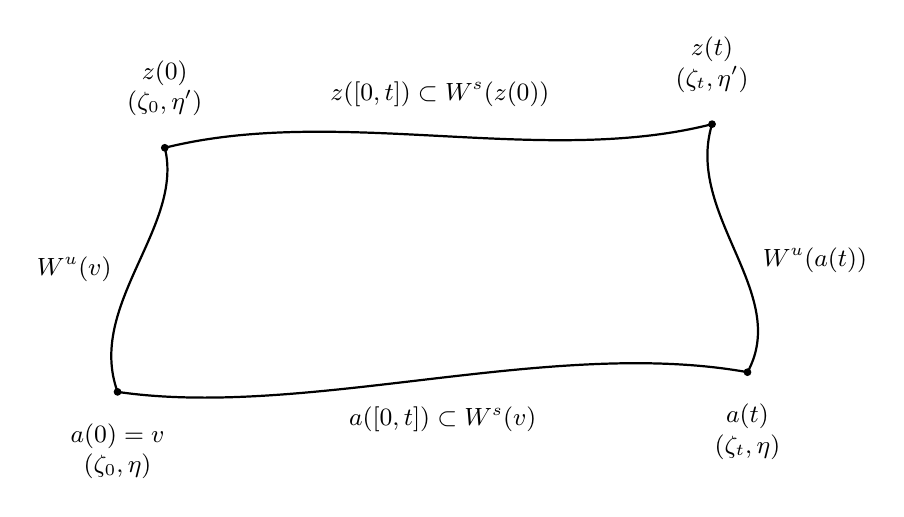
\begin{tikzpicture}[x=1cm,y=1cm,font=\small]
  \coordinate (v) at (0,0);
  \coordinate (a) at (8,0.25);
  \coordinate (z0) at (0.6,3.1);
  \coordinate (zt) at (7.55,3.4);
  \draw[thick] (v) .. controls (2.4,-0.35) and (5.5,0.7) .. (a)
    node[pos=0.52,below=7pt] {$a([0,t])\subset\Ws(v)$};
  \draw[thick] (z0) .. controls (2.8,3.65) and (5.4,2.85) .. (zt)
    node[pos=0.50,above=7pt] {$z([0,t])\subset\Ws(z(0))$};
  \draw[thick] (v) .. controls (-0.4,1.1) and (0.85,2.1) .. (z0)
    node[pos=0.49,left=5pt] {$\Wu(v)$};
  \draw[thick] (a) .. controls (8.55,1.25) and (7.2,2.25) .. (zt)
    node[pos=0.47,right=5pt] {$\Wu(a(t))$};
  \fill (v) circle (1.4pt);
  \fill (a) circle (1.4pt);
  \fill (z0) circle (1.4pt);
  \fill (zt) circle (1.4pt);
  \node[below=8pt,align=center] at (v)
    {$a(0)=v$\\$ (\zeta_0,\eta)$};
  \node[below=8pt,align=center] at (a)
    {$a(t)$\\$ (\zeta_t,\eta)$};
  \node[above=8pt,align=center] at (z0)
    {$z(0)$\\$ (\zeta_0,\eta')$};
  \node[above=8pt,align=center] at (zt)
    {$z(t)$\\$ (\zeta_t,\eta')$};
\end{tikzpicture}
\caption{Actual leaf incidences in the infinite-dimensional alternative,
for a fixed finite $t$. Each ordered pair gives the past and future
endpoints. The lower path is tangent to $P^s$; the translated upper
path is proved tangent to $E^s$. Each vertical connection indicates
membership in one strong unstable leaf. The drawing is schematic:
it asserts no ambient affine plane, smooth product chart or embedded
surface. The contradiction uses the proper lower ray and the endpoint
identities, not any geometric shape of this drawing.}
\label{fig:mixed-rectangle}
\end{figure}


We claim
\begin{equation}\label{real:busemann-divergence}
 b_{\zeta_t}(a(t))\longrightarrow-\infty.
\end{equation}
The sum $b_\eta+b_{\zeta_t}$ is convex and has zero gradient on
the geodesic with these endpoints, so it attains its minimum
there. Let $c(r)$ be the ray from $o$ toward $\eta$. For each
fixed $r>0$,
\[
 b_\eta(a(t))+b_{\zeta_t}(a(t))
      \le b_\eta(c(r))+b_{\zeta_t}(c(r)).
\]
As $t\to\infty$ the right-hand side tends to $-2r$, by endpoint
continuity of normalized Busemann functions. The term
$b_\eta(a(t))=b_\eta(v)$ is fixed. Since $r$ is arbitrary,
\eqref{real:busemann-divergence} follows.

On the other hand, $z(t)$ has ordered endpoints
$(\zeta_t,\eta')$ and fixed future Busemann level
$b_{\eta'}(z(0))$. Their limiting pair $(\eta,\eta')$ is off the
diagonal. The corresponding unit tangent vectors therefore
converge to the vector with this limiting pair and that level;
in particular they remain in a compact subset of
$S\widetilde M$. Endpoint continuity now makes
$b_{\zeta_t}(z(t))$ bounded. But $z(t)\in\Wu(a(t))$ means that
the two vectors have the same past endpoint and past Busemann
level, so
\[
 b_{\zeta_t}(z(t))=b_{\zeta_t}(a(t)).
\]
This contradicts \eqref{real:busemann-divergence} and excludes
the infinite-dimensional alternative.
\end{proof}

\section{From formal sign fields to a smooth splitting}
\label{smooth:section}

The finite alternative in Theorem~\ref{alg:dichotomy} remains.  In this
section all work on the universal cover is local in the resulting smooth
structure, so the conclusions descend to $SM$.  We first recover the actual
plaque jets on an entire typical axis.  We then propagate their regularity
using scalar functions which label weak unstable leaves.

\subsection{Actual plaque jets and formal leaf labels}

\begin{lemma}[Tangency to the central plaques]
\label{smooth:tangency}
In the finite alternative, the positive-$D$ invariant formal plane field is
tangent to the entire formal central unstable plaque.  Consequently, on each
entire typical strong stable leaf, all finite Taylor jets of the actual weak
unstable plaques are smooth functions of their crossing point.  They have
holonomic full formal extensions there.  The same statements hold on the
weak stable leaf generated by that strong stable leaf.
\end{lemma}

\begin{proof}
Use the graded section coordinates of Lemma~\ref{sym:graded-contact}
and the dilation of Proposition~\ref{sym:dilation}.  Write $x$ for the positive variables and $y$ for
the negative variables.  The actual central unstable plaque has formal
projection $y=0$.  Let $D_+$ and $D_-$ denote the restrictions of $D$ to the
two coordinate spaces.  The positive formal field furnished by
Proposition~\ref{alg:axis-coherence} has value $E^u$ at the origin and is invariant
under the dilation.  Its restriction to $y=0$ is a graph, with graph matrix
$B(x)$ from the positive to the negative space.  Dilation invariance gives
\[
 B(e^{tD_+}x)=e^{tD_-}B(x)e^{-tD_+}.
\]
Diagonalize $D$ over the real graded spaces.  A monomial $x^\nu$ in a matrix
entry with input weight $\lambda_i>0$ and output weight $\mu_j<0$ would
have to satisfy
\[
 \sum_a\nu_a\lambda_a=\mu_j-\lambda_i<0.
\]
The left side is nonnegative, so every coefficient vanishes.  Thus $B=0$.
This is an identity of formal series; it needs no convergence.  Adding the
flow direction gives formal tangency to the weak unstable plaque.

In ordinary smooth coordinates, represent that plaque by a graph $z=g(v)$
with prescribed crossing $g(0)$.  Tangency to the formal plane field gives a
system
\[
 \partial_{v_i}g(v)=A_i(v,g(v)).
\]
Its constant coefficient determines the first derivatives of $g$; after
$d$ differentiations, it determines derivatives of order $d+1$ from the
field jet and the already determined graph coefficients.  There is no
existence assertion hidden in this recursion: the actual central plaque
already provides the formally tangent solution.  The recursion merely
expresses each of its graph coefficients by finitely many operations on
the ambient formal field jet.

The full ambient jets of that field are smooth and holonomic on each
entire typical stable axis, by Proposition~\ref{alg:axis-coherence}.  Hence the
recursively obtained graph coefficients are smooth there and have the
same tangential coherence.  Initially the equality with actual plaque
coefficients holds at the regular crossing points.  It holds everywhere
on the axis by continuity: the actual plaques depend continuously in
$C^0$ on their crossings, have uniformly bounded local derivatives of
each finite order, and therefore depend continuously in each finite
$C^r$ norm by interior interpolation.  Regular crossings are dense on the
axis by conditional full measure.  This also explains why no transverse
smoothness of the actual foliation was used.  Flow transport proves the
weak-axis assertion, with compatibility on overlapping flow boxes.
\end{proof}

Fix one such strong stable leaf $A^{\mathrm{all}}$ on the universal cover,
with future endpoint $\eta$.  Normalize its Busemann function so that
$A^{\mathrm{all}}$ is at height $b_\eta=0$; our convention is
$b_\eta(\pi\phi_t v)=b_\eta(\pi v)-t$ when $v_+=\eta$.
The past-endpoint map identifies this leaf with
$\partial_\infty\widetilde M\setminus\{\eta\}$.  Choose a coordinate patch
$A\subset A^{\mathrm{all}}$, with smooth coordinates $a\mapsto q_A(a)\in
\R^m$, and write
\[
 \mathcal B=\{\phi_t a:a\in A,\ t\in\R\}.
\]
This is an open part of the fixed-future weak stable leaf.  On the open
set $\mathcal U$ of vectors whose past endpoints occur in $A$, define
\begin{equation}
 \label{smooth:label-definition}
 q(v)=q_A(a(v)),\qquad a(v)_-=v_-,\quad a(v)\in A.
\end{equation}
The endpoint identifications show that $q$ is continuous.  It is constant
on actual weak unstable leaves and under the flow.  Only its restriction
$q_0=q|_{\mathcal B}$ is known to be smooth at this stage.

\begin{lemma}[Formal inversion of plaque labels]
\label{smooth:formal-labels}
The function $q_0$ has a distinguished full formal ambient extension along
$\mathcal B$.  Its coefficients are smooth and holonomic on $\mathcal B$,
it is formally constant on every actual weak unstable plaque crossing
$\mathcal B$, and its finite jets transform by scalar pullback under the
flow.  These assertions concern formal jets along $\mathcal B$, and do
not assert differentiability of $q$ elsewhere.
\end{lemma}

\begin{proof}
At any fixed Busemann height, the strong stable slice in $\mathcal B$ is a
smooth transversal to the weak unstable plaques.  Use coordinates $a$ on
this slice and auxiliary variables $z$ along the plaques.  By
Lemma~\ref{smooth:tangency}, the parameterized actual plaque Taylor graphs
form a formal map
\[
 \Psi(a,z),\qquad \Psi(a,0)=a,
\]
whose coefficients in $z$ are smooth in $a$, with all their tangential
derivatives. Within a weak unstable plaque, the strong plaque through
its crossing is tangent to $\ker\alpha$. Its graph coefficients are
determined recursively from the weak plaque jets and the smooth contact
form, as in Lemma~\ref{smooth:tangency}; the actual strong plaque supplies
the solution. These finite operations preserve smooth dependence on $a$.
We may therefore choose $z=(u,t)$ and write
\[
 \Psi(a,u,t)=\phi_t\Gamma(a,u),\qquad \Gamma(a,0)=a,
\]
where $\Gamma(a,u)$ is the actual strong unstable plaque Taylor map
through $a$. Only its finite Taylor coefficients and their smooth
dependence on $a$ are used. The differential of $(a,z)\mapsto\Psi(a,z)$ at $z=0$ is
invertible, by transversality.  Formal inversion therefore determines
$a=a(p)$ and the scalar formal function $q_0|_{\mathrm{slice}}(a(p))$
to every finite order.  Concretely, to compute order $r$, take a sufficiently high finite
Taylor polynomial of $\Psi$ in $z$ and invert it as an ordinary local
smooth map.  The resulting order-$r$ jet is independent of all higher
coefficients.  Thus this construction uses only finitely many jet
operations at each stage.

Smooth dependence of the coefficients on $a$ gives tangential
holonomicity of the inverse jets.  The construction is independent of
coordinates because it describes the crossing of an actual plaque with
the chosen transversal.  Moving the height slice by the flow transports
both the actual plaque jets and the prescribed labels; formal inversion
commutes with this transport.  This proves compatibility at different
heights. The inverse label is independent of $u,t$, and
$\partial_t\Psi=X\circ\Psi$ gives the full formal identity $Xq=0$.
Differentiating scalar jet equivariance in time therefore gives the
holonomic derivative identity along $X$; combined with coherence on
each height slice, this proves full holonomicity along $\mathcal B$.
In particular, the scalar jet identity is
\[
 j^r_p q=(j^r_{\phi_t p}q)\circ j^r_p\phi_t,
 \qquad p,\phi_t p\in\mathcal B,
\]
where both $q$-jets in this display mean the formal jets just constructed.
\end{proof}

\subsection{Backward geometry and estimates along the axis}

Let $N_\eta(x)=(x,v_\eta(x))$ be the unit vector based at $x$ pointing
toward $\eta$.  It parametrizes the fixed-future weak stable leaf as a
smooth graph over $\widetilde M$.  This graph, its local charts, and all
of its fixed-order local derivatives have uniform bounds.  Indeed the
individual weak stable leaves have uniform smooth plaque bounds, and
their spatial projections have uniformly invertible differentials.
Write $\rho(x,v)=N_\eta(x)$.  Near this graph use the intrinsic angular
coordinate
\[
 t= v-\langle v,v_\eta(x)\rangle v_\eta(x)
       \in v_\eta(x)^\perp,
 \qquad \langle v,v_\eta(x)\rangle>0.
\]
It is the tangential component of $v$ in the horosphere.  Thus
$v=\sqrt{1-|t|^2}\,v_\eta(x)+t$.  The degree-$l$ angular Taylor
coefficient of the formal label will be denoted $q_l$; it is a smooth
symmetric $l$-tensor on the horosphere tangent bundle over $\mathcal B$,
with values in $\R^m$, and includes the Taylor factorial.  In these
coordinates the formal label is $\sum_{l\geq0}q_l(s,r)[t^l]$, where $r$
is Busemann height and $s$ denotes coordinates on its horosphere.

\begin{lemma}[Compact sets approach the fixed-future axis]
\label{smooth:backward-geometry}
Let $K\Subset\mathcal U$.  There are $b>0$, $C<\infty$, and a compact
$K_{\mathcal B}\Subset\mathcal B$ such that, for all sufficiently large
$n$ and $v\in K$,
\[
 |t(f^{-n}v)|\leq Ce^{-bn},\qquad
 f^n\rho(f^{-n}v)\in K_{\mathcal B}.
\]
The actual weak unstable plaque through $f^{-n}v$ crosses the axis
$t=0$ at the same Busemann height, at a point $a_n(v)$.  That crossing
and the axis points underlying the intervening local plaque graph also
have their $f^n$-images in $K_{\mathcal B}$, after enlarging this compact
set.  All assertions hold on a fixed neighborhood of $K$.
\end{lemma}

\begin{proof}
The crossing $a(v)$ in \eqref{smooth:label-definition} depends
continuously on $v$, so $a(K)$ is compact in $A$.  Put $\zeta=v_-$ and
choose the continuous bounded time shift
\[
 \tau(v)=b_\zeta(\pi v)-b_\zeta(\pi a(v)).
\]
The vector $z(v)=\phi_{\tau(v)}a(v)$ has the same past endpoint and the
same past Busemann height as $v$; hence it is on its strong unstable
leaf.  Moreover their intrinsic strong unstable distance is uniformly
bounded on $K$.  To see the uniformity explicitly, join their base
points by a spatial geodesic segment of bounded length and project it
onto their common past horosphere along the Busemann gradient flow.
The required flow times are bounded by the segment length.  Uniform
bounds for the Busemann Hessian bound the length of this projected path
and its lift to the normal graph.  This uses the fixed negatively
curved metric, not regularity of the endpoint map.

Backward strong unstable contraction now gives
\[
 d^u(f^{-n}v,f^{-n}z(v))\leq Ce^{-bn}.
\]
Write $f^{-n}v=(x_n,v_n)$ and $f^{-n}z(v)=N_\eta(y_n)$.
The uniform local bounds of $N_\eta$ imply
$d(N_\eta(x_n),N_\eta(y_n))\leq Ce^{-bn}$ and the asserted angular
bound.  If
\[
 \epsilon_n=b_\eta(x_n)-b_\eta(y_n),
\]
then $|\epsilon_n|\leq Ce^{-bn}$.  The two vectors
$\phi_{\epsilon_n}N_\eta(x_n)$ and $N_\eta(y_n)$ belong to the same
strong stable leaf and have intrinsic distance $O(e^{-bn})$.
Forward strong stable contraction, and the unchanged small time shift,
show that $f^nN_\eta(x_n)$ stays within $O(e^{-bn})$ in the intrinsic
weak stable metric of the compact family $z(v)$.  This proves the
compact-axis assertion.

For completeness, the local crossing assertion has a uniform
transversality bound.  At $t=0$, the weak unstable plaque intersected with
$b_\eta=r$ has tangent $E^u$.  In Jacobi coordinates the differential of
its angular coordinate in a spatial direction $a$ is
$(U(v)+U(-v))a$, which is uniformly positive definite.  Uniform smooth
bounds on individual plaques and the inverse function theorem therefore
give actual graphs
\begin{equation}
 \label{smooth:actual-graphs}
 s=P_{s_0,r}(t),\qquad P_{s_0,r}(0)=s_0,
\end{equation}
on a fixed radius, with uniformly bounded derivatives in $t$ of each
fixed order.  No derivative with respect to $s_0$ is asserted.

The nearby crossing of the plaque through $f^{-n}v$ is especially
explicit.  If $c_n=b_\eta(x_n)$, then
\[
 c_n=nT-\tau(v)+\epsilon_n,
 \qquad a_n(v)=\phi_{-c_n}a(v),
 \qquad f^na_n(v)=\phi_{\tau(v)-\epsilon_n}a(v).
\]
These identities follow from its past endpoint, future endpoint, and
height.  They prove compactness of its forward image.  On the local
graph between angular values $0$ and $t(f^{-n}v)$, the base points move
by $O(e^{-bn})$ on this same horosphere.  Their axis vectors have that
small intrinsic stable distance from $a_n(v)$; contraction gives the
remaining compactness assertion.  Replacing $K$ by a slightly larger
compact subset of $\mathcal U$ proves the neighborhood assertion.
\end{proof}

All following norms along the axis are computed in uniformly bounded
local weak stable charts and uniformly bounded tensor frames.  For
$L\Subset\mathcal B$ let $L_n=f^{-n}L$.  When an interior estimate is
used, enlarge $L$ slightly inside $\mathcal B$. The forward weak-plaque
bounds in Lemma~\ref{pre:plaque-contraction}, in particular the uniform
Lipschitz bound, give a uniform positive amount of local room around $L_n$.

\begin{lemma}[A derivative-order-independent exponential bound]
\label{smooth:naive}
For each angular degree $l$ there is $A_l<\infty$ such that, for every
$j\geq0$ and every $L\Subset\mathcal B$,
\begin{equation}
 \label{smooth:naive-bound}
 \|q_l\|_{C^j(L_n)}\leq C_{L,l,j}e^{A_ln}.
\end{equation}
The exponent $A_l$ is independent of $j$.
\end{lemma}

\begin{proof}
Transport the full ambient scalar jet of order $l$ from $f^np$ to $p$,
using Lemma~\ref{smooth:formal-labels}.  The one-step transport is a
finite-dimensional linear pullback-jet matrix $M_l(p)$.  In uniformly
bounded geometric charts these matrices and every fixed-order weak-axis
derivative are uniformly bounded: the one-step ambient map is smooth,
and the weak-axis charts have the uniform leafwise bounds just
explained.  The transport over $n$ steps is the product of these matrices
at $p,fp,\ldots,f^{n-1}p$.

When this product is differentiated $j$ times along the initial weak
axis, at most $j$ factors are differentiated.  Each derivative of a
factor composed with $f^i|_{\mathcal B}$ is bounded by a constant
depending on $l,j$, uniformly in $i$.  The remaining factors are bounded
by a fixed $M_l\geq1$.  The number of terms is at most a constant times
$(1+n)^j$.  The final jet field on $L$, and its derivatives composed with
$f^n|_{\mathcal B}$, have bounded derivatives.  Hence the product rule
gives $C_{L,l,j}(1+n)^jM_l^n$.  Absorb the polynomial in $e^n$, with its
$j$-dependent prefactor.  Taking angular coefficients and changing
uniform frames preserve the resulting exponent $A_l=1+\log M_l$.
This is Lemma~\ref{real:product-derivatives} on the fixed bundle
$J^l$ of scalar $l$-jets: differentiation changes the matrix
coefficient functions, not the jet order. Using ambient derivative bounds
for $f^n$ in its place would lose the independence from $j$.
\end{proof}

\begin{lemma}[Subexponential bounds for every axis derivative]
\label{smooth:subexponential}
For every $l,j\geq0$, every $\varepsilon>0$, and every
$L\Subset\mathcal B$ there is a constant $C_{L,l,j,\varepsilon}$ such
that
\begin{equation}
 \label{smooth:subexponential-bound}
 \|q_l\|_{C^j(L_n)}
 \leq C_{L,l,j,\varepsilon}e^{\varepsilon n}.
\end{equation}
\end{lemma}

\begin{proof}
We induct on $l$, proving all derivative orders at each stage.  For
$l=0$, the identity $q_0(p)=q_0(f^np)$ and the bounded weak-axis
derivatives of forward iterates give bounded derivatives on $L_n$.

At each fixed height, formal constancy on the actual graph
\eqref{smooth:actual-graphs} gives the coefficientwise identity
\begin{equation}
 \label{smooth:crossing-identity}
 \sum_{k\geq0}q_k(P_{s_0,r}(t),r)[t^k]=q_0(s_0,r).
\end{equation}
Every occurrence of a coefficient on the left is Taylor-expanded at
$t=0$.  The identity follows directly from the formal crossing inversion
of Lemma~\ref{smooth:formal-labels} and its tangential holonomicity.
In degree $l$, its only term containing $q_l$ is
$q_l(s_0,r)[t^l]$.  All other terms involve derivatives in $s$ of $q_k$
with $k<l$ and order at most $l-k$, multiplied by polynomials in the
$t$-derivatives of $P_{s_0,r}$ through order $l$.  These graph derivatives
are uniformly bounded.  The induction hypothesis and polarization of
the homogeneous degree-$l$ identity therefore give
\[
 \|q_l\|_{C^0(L_n)}\leq C_{L,l,\varepsilon}e^{\varepsilon n}
 \quad\hbox{for every }\varepsilon>0.
\]
This argument estimates only values of the next coefficient.  In
particular it never differentiates the actual graph with respect to its
crossing point.

We upgrade values to arbitrary weak-axis derivatives using interpolation
on the full weak axis, including the height coordinate.  On a fixed
interior chart the elementary Taylor difference estimate is
\[
 \|D^ju\|_{C^0}
 \leq C_{j,r}\bigl(h^{-j}\|u\|_{C^0}
                 +h^{r-j}\|u\|_{C^r}\bigr),
 \qquad 0<h<h_0,
\]
where the norms on the right are on a slightly larger chart.  The
uniform interior room makes its constants independent of $n$; see also
Lemma~\ref{real:interpolation}.  Fix $j\geq1$ and target
$\varepsilon>0$.  Take $\delta=\varepsilon/(4j)$ and
$h=e^{-\delta n}$, use the value bound with exponent $\varepsilon/4$,
and choose a fixed integer $r>j+A_l/\delta$.  By
\eqref{smooth:naive-bound}, the two terms then have exponents at most
$\varepsilon/2$ and $A_l-\delta(r-j)<0$, respectively.  This proves
\eqref{smooth:subexponential-bound}.  The choice of $r$ is possible
precisely because $A_l$ does not depend on $r$.  The argument works for
every compact $L$, using a larger compact for interior estimates, so the
induction is complete.
\end{proof}

\subsection{Smoothness of the actual label}

\begin{proposition}[Propagation from the axis]
\label{smooth:propagation}
The actual endpoint label $q:\mathcal U\to\R^m$ is smooth.
\end{proposition}

\begin{proof}
Fix nested compact neighborhoods $K\Subset K^+\Subset\mathcal U$.
For large $n$, Lemma~\ref{smooth:backward-geometry} puts $f^{-n}K^+$ in
the angular coordinate neighborhood of the axis.  For a fixed finite
cutoff $R$ define the smooth function, near $K^+$,
\begin{equation}
 \label{smooth:approximants}
 p_{n,R}(v)=\sum_{l=0}^R
 q_l\bigl(\rho(f^{-n}v)\bigr)
       \bigl[t(f^{-n}v)^l\bigr].
\end{equation}
These expressions are intrinsic tensor contractions, so no seams from
angular frames occur.  They use a finite polynomial at each $n$; no
infinite formal series is evaluated.

We first estimate their error without differentiating $q$.  At a pulled
back point, use its actual plaque graph
$s=P_{s_0,r}(t)$ and its genuine crossing $(s_0,r,0)$.  The function of
the angular parameter
\[
 H(t)=\sum_{l=0}^R q_l(P_{s_0,r}(t),r)[t^l]-q_0(s_0,r)
\]
has zero Taylor coefficients through degree $R$ by
\eqref{smooth:crossing-identity}.  Along the segment from zero to the
angular parameter in question, all underlying axis points lie over the
compact set supplied by Lemma~\ref{smooth:backward-geometry}.
Lemma~\ref{smooth:subexponential}, the uniform derivatives of the
single actual graph, and Taylor's remainder formula give
\[
 |H(t)|\leq C_{K,R,\varepsilon}e^{\varepsilon n}|t|^{R+1}.
\]
The actual label equals $q_0(s_0,r)$ on that plaque, and is flow
invariant.  Consequently
\begin{equation}
 \label{smooth:approximation-error}
 \|p_{n,R}-q\|_{C^0(K^+)}
 \leq C_{K,R,\varepsilon}
       e^{-(b(R+1)-\varepsilon)n}.
\end{equation}
Only derivatives of the smooth axis coefficients and of an individual
actual plaque entered this estimate.

For each fixed $j$, the same coefficients have subexponential
$C^j$ bounds.  A polynomial of degree at most $R$ in $|t|<1$ therefore
has a $C^j$ bound $C_{K,R,j,\varepsilon}e^{\varepsilon n}$ in the
geometric angular coordinates.  The ordinary ambient bounds for
$f^{-n}$ and the chain rule give
\begin{equation}
 \label{smooth:approximant-growth}
 \|p_{n,R}\|_{C^j(K^+)}
 \leq C_{K,R,j,\varepsilon}e^{(B_j+\varepsilon)n},
\end{equation}
where $B_j$ depends on $j$ and the smooth dynamics, but is independent
of $R$.  Indeed differentiating the angular polynomial at most $j$
times only introduces $R$-dependent combinatorial constants; its
coefficients already have arbitrary subexponential slack.  All
exponential losses come from derivatives of $f^{-n}$ of orders at most
$j$.  This independence from $R$ is the second essential exponent
separation in the proof.

Here are the convergence quantifiers.  Fix a desired derivative order
$j\geq1$ and a desired positive convergence rate $\lambda$.  Set
$r=2j+2$, take $\varepsilon=1$, and choose one finite $R$ large enough
that
\[
 \bigl(b(R+1)-1\bigr)(1-j/r)
       -(B_r+1)j/r>\lambda.
\]
The differences $p_{n+1,R}-p_{n,R}$ have the $C^0$ decay in
\eqref{smooth:approximation-error} and the $C^r$ growth in
\eqref{smooth:approximant-growth}.  Interior interpolation on the fixed
pair $K\Subset K^+$ gives
\[
 \|p_{n+1,R}-p_{n,R}\|_{C^j(K)}\leq C e^{-\lambda n}.
\]
Thus the sequence converges in $C^j(K)$ to its already identified
uniform limit $q$.  Since $j$ is arbitrary, $q$ is smooth.  There is no
requirement that a single cutoff work for all $j$.  If a single sequence
converging in the $C^\infty$ topology is desired, choose cutoffs $R_k$
which work through order $k$, and choose $n_k$ so large that
$\|p_{n_k,R_k}-q\|_{C^k(K)}\leq2^{-k}$.  This diagonal sequence has that
property and still evaluates only finite polynomials.
\end{proof}

\subsection{Nondegeneracy and the strong bundles}

Smoothness of a leaf label does not by itself make its differential
surjective.  We use bounded holonomy Jacobians for this final step.

\begin{lemma}[Volume comparison for weak unstable holonomy]
\label{smooth:holonomy-volume}
Between two smooth $m$-dimensional local transversals to the weak
unstable foliation, its holonomy $h$ satisfies, locally,
\[
 c\,\Vol(E)\leq\Vol(h(E))\leq C\,\Vol(E)
\]
for measurable sets $E$, with $0<c\leq C<\infty$.
\end{lemma}

\begin{proof}
Strong unstable holonomy between smooth transversals is absolutely
continuous with locally bounded positive Jacobian; applying the same
statement to inverse holonomy supplies the reciprocal bound.  This is
the bounded-Jacobian theorem for horospheric foliations
\cite[Appendix, Theorem~5.1 and Definition~3.3]{Ballmann1995}.
We explain the passage to the weak foliation.

Thicken each transversal for a short interval by the flow, using a fixed
time translate of the target if necessary.  The resulting smooth
$(m+1)$-dimensional submanifolds are transversals to the strong unstable
foliation.  On suitably small flow boxes, strong holonomy has the form
\[
 H(a,t)=(h(a),t+\tau(a)).
\]
This follows from flow invariance and uniqueness of the crossing;
$\tau$ need only be continuous.  Choose a fixed short interval $I$ so
that $H$ is defined on $E\times I$ for every $E$ in a smaller source
patch.  In product coordinates, its image has the interval
$I+\tau(h^{-1}(y))$ above each $y\in h(E)$.  Fubini's theorem gives
product volume $|I|\Vol(h(E))$.  The smooth volume densities of both
flow-box parametrizations are bounded above and below.  The strong
holonomy comparison applied to $E\times I$ proves the displayed weak
comparison.  A finite chain of boxes proves the same assertion along
any compact holonomy path.
\end{proof}

\begin{theorem}[Smoothness of the Anosov splitting]
\label{smooth:splitting}
In the finite alternative of Theorem~\ref{alg:dichotomy}, the actual
bundles $E^u$ and $E^s$ are smooth on $SM$.
\end{theorem}

\begin{proof}
Fix a base point $x$ on the universal cover.  On its direction sphere,
the restriction $q|_{S_x\widetilde M}$ is locally the weak unstable
holonomy to $A$, followed by the smooth coordinate map $q_A$.  Both are
genuine $m$-dimensional transversals: a weak unstable tangent vector
with zero spatial projection is zero, and $TA=E^s$ is complementary to
$E^u\oplus\R X$.  The restriction is a local
homeomorphism, by the endpoint parametrizations.  By
Proposition~\ref{smooth:propagation} it is smooth, and by
Lemma~\ref{smooth:holonomy-volume} it satisfies a positive lower volume
comparison on every smaller patch.

Its derivative cannot be singular. Use smooth coordinate charts on
the source sphere and the target, with volume densities bounded above
and below. If the derivative at a point had rank less than $m$, choose
a unit target direction perpendicular to its image. Differentiability
then places the image of a coordinate ball of radius $r$ in a box with
widths $O(r)$ in the other $m-1$ directions and $o(r)$ in that direction.
Its volume is $o(r^m)$, contradicting the fixed positive lower volume
comparison for these balls. Thus $dq$ is surjective at every point of
$\mathcal U$.  The smooth bundle $\ker dq$ has dimension $m+1$ and
contains the tangent spaces of the actual weak unstable leaves, since
$q$ is constant on each such smooth leaf.  The dimensions agree, so
\[
 \ker dq=E^u\oplus\R X
 \quad\hbox{on }\mathcal U.
\]
Intersecting with the smooth contact distribution gives the smooth
strong unstable bundle
\[
 E^u=(\ker dq)\cap\ker\alpha.
\]

The coordinate patches of the full typical strong stable axis cover
all past endpoints except $\eta$.  A second typical axis with a distinct
future endpoint covers the omitted endpoint.  Such an axis exists
because typical points have full smooth measure, whereas a single
fixed-future weak leaf has positive codimension.  The preceding
argument therefore gives smoothness of $E^u$ everywhere on the cover.
The flip $v\mapsto-v$ exchanges the strong bundles, and hence gives
smoothness of $E^s$.  These are the actual invariant bundles, so they
are deck invariant and descend smoothly to $SM$.
\end{proof}


\section{Completion of the proof}
\label{sec:completion}

Theorem~\ref{smooth:splitting} supplies the global smoothness required
by Proposition~\ref{pre:smooth-rigidity}. We first prove that classical
implication, then assemble the entropy-rigidity theorem and its converse.

\begin{proof}[Proof of Proposition~\ref{pre:smooth-rigidity}]
Smoothness of the weak stable distribution lets us apply the theorem
of Benoist--Foulon--Labourie
\citep[Theorem~2]{BenoistFoulonLabourie1992}. It supplies a smooth
conjugacy to a negatively curved locally symmetric geodesic flow on
the unit tangent bundle of a closed manifold $(M_0,g_0)$, with the
scale absorbed in the model metric. We first explain how their general
contact formulation leads to this geodesic conclusion: its finite-cover
and closed-one-form qualifications
\citep[Theorem~1bis and Sections~7.1--7.5]{BenoistFoulonLabourie1992}
reduce to a constant time change on finite covers. The geodesic
specialization in Section~7.5.3 gives a torsion-free group and hence a
manifold model. After explaining that reduction, we recover the base
metric from contact volume and minimal entropy rigidity.

For $n\ge3$, the sphere-bundle exact sequence gives
$\pi_1(SM)\simeq\pi_1(M)$ because $S^{n-1}$ is simply connected,
and the same holds on the symmetric model. Hence finite covers of
these unit tangent bundles come from finite base covers.

On $SM_0$, a canonical time density is
$a_0+\beta(X_0)>0$, where $a_0>0$ and $\beta$ is a closed
one-form on $SM_0$. Its period in a conjugacy class $\gamma$ is
\[
 a_0\ell_0(\gamma)+\int_\gamma\beta.
\]
Geodesic periods agree for inverse classes. The group isomorphism
induced by the conjugacy respects inversion, whereas the integral
of $\beta$ changes sign. Thus its integral vanishes on every
closed geodesic lift. Since $\pi_1(SM_0)\simeq\pi_1(M_0)$,
these lifts, including iterates, represent every nontrivial
conjugacy class in $SM_0$. All periods of $\beta$ therefore vanish,
and $\beta=db$.
The orbit shift
\[
 x\longmapsto\phi^0_{b(x)/a_0}(x)
\]
carries $X_0/(a_0+X_0b)$ to $X_0/a_0$. It is a diffeomorphism:
its orbit derivative is positive, and its bounded time displacement
makes it onto on nonperiodic orbits and degree one on periodic
orbits. This removes the exact correction.

We therefore have, on finite covers when necessary, a diffeomorphism
$\Psi$ with $\Psi_*X_g=aX_0$ for a constant $a>0$. Strong stable
and unstable distributions are carried to their counterparts.
Evaluation on these distributions and on $X_g$ gives
\[
 \Psi^*\alpha_0=a\alpha_g,
 \qquad
 \Psi^*\bigl(\alpha_0\wedge(d\alpha_0)^{n-1}\bigr)
 =a^n\alpha_g\wedge(d\alpha_g)^{n-1}.
\]
The fiber integral of contact volume is the same universal multiple
of base Riemannian volume on both sides. Consequently
\[
 \Vol(g_0)=a^n\Vol(g),
 \qquad \htop(g)=a\htop(g_0).
\]
The bases are aspherical, so the induced group isomorphism is realized
by a base homotopy equivalence. In particular,
$H_n(M_0;\mathbb Z)\simeq H_n(M;\mathbb Z)=\mathbb Z$,
because the source base is oriented. Hence $M_0$ is orientable,
and this equivalence has degree of absolute value one.

Topological entropy agrees with volume entropy in negative
curvature \citep{Manning1979}; see also
\citet[Main Theorem, parts~(a)--(b)]{Leuzinger2006}.
Set $\widehat g=a^2g$ and write $h_{\mathrm{vol}}$ for volume entropy.
The scaling identities give
\[
 \Vol(\widehat g)=\Vol(g_0),\qquad
 h_{\mathrm{vol}}(\widehat g)=h_{\mathrm{vol}}(g_0).
\]
The normalized equality case of minimal entropy rigidity now gives
a Riemannian covering from $(M,\widehat g)$ to $(M_0,g_0)$
\citep[Theorem~8.1 and Proposition~8.2]{BessonCourtoisGallot1995}.
For the Cayley case we use the corrected determinant estimate and
equality argument in \citet[arXiv version~1, final paragraph of
Section~3 and Section~4.4]{Ruan2024}.
Thus $g$ is homothetic to the symmetric metric, and local symmetry
descends from the covers.
One may alternatively use the direct smooth-foliation conclusion
of \citet[Corollary~9.17]{BessonCourtoisGallot1995} with the same
Cayley correction.
\end{proof}

\begin{proof}[Proof of Theorem~\ref{thm:main}]
Suppose first that the entropies are equal.
Proposition~\ref{pre:entropy-forms} provides the transported conormal
volumes. Theorem~\ref{hull:main} constructs their coherent formal
affine fields. Proposition~\ref{sym:effective} and
Theorem~\ref{alg:dichotomy} give the algebraic alternative.
Proposition~\ref{real:infinite-excluded} excludes its
infinite-dimensional case. In the finite-dimensional case,
Theorem~\ref{smooth:splitting} proves that $\Es$ and $\Eu$
are smooth on all of $SM$. Proposition~\ref{pre:smooth-rigidity}
therefore gives $\nabla^gR_g=0$.

Conversely, suppose that $\nabla^gR_g=0$. Completeness makes the
simply connected cover globally symmetric. Strict negative curvature
excludes nontrivial products, compact type and flats of dimension two;
the cover is therefore of noncompact type and rank one
\citep[Theorem~1.3.5, Section~1.6 and Section~3.3]{Gorodski2021}.
Its isotropy is transitive on unit tangent directions
\citep[Section~9, Theorem~9 and its rank-one consequence]{EschenburgSymmetricSpaces}.
Together with homogeneity, this shows that the curvature operator has
the same negative eigenvalue list at every unit tangent vector.
Parallel curvature makes that operator constant in a parallel normal
frame along each geodesic.
The unstable Riccati solution is $U(v)=\sqrt{-R_v}$, the positive
definite square root. Thus $J=\tr U$ is a constant, say $h_0$.
By Proposition~\ref{pre:entropy-forms}, or directly by the entropy
formula and inequality, Liouville volume is an equilibrium state for
$-J$ and this potential has pressure zero. Since $-J=-h_0$ is
constant, $\htop(\phi_1)=h_0=h_{m_L}(\phi_1)$.
Both implications are unchanged by finite isometric covers and
overall rescaling.
\end{proof}

\bibliographystyle{plainnat}
\bibliography{references}
\end{document}
